\section{Baselines Details}
\label{sec:baseline_appendix}

In this section, we include additional information about the baselines evaluated and analyzed in the main paper: the visuomotor control baseline and two variants of the baselines using action primitives, with and without the history of observations.

\begin{figure}[t]
    \centering
    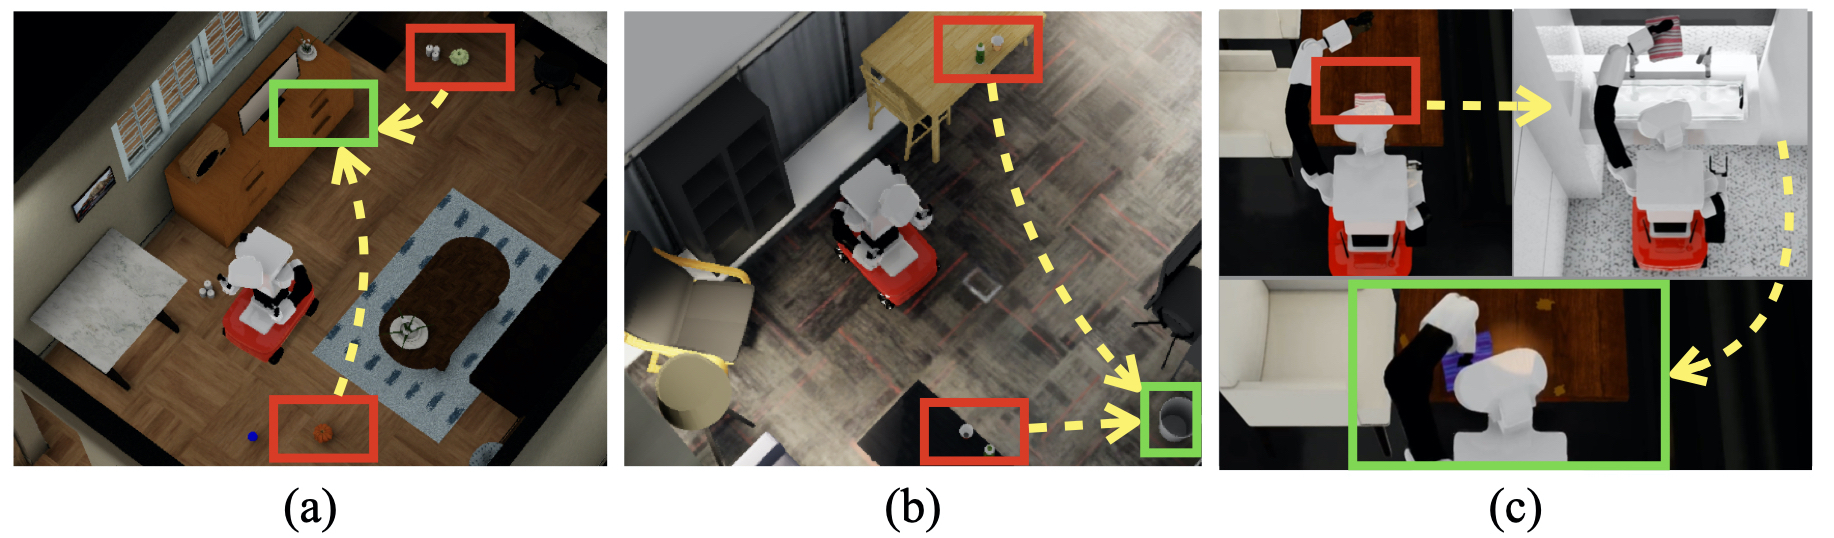
\includegraphics[width=0.95\textwidth]{figures/baseline_appendix/baseline-task.jpeg}
    \caption{\textbf{Activities used in our evaluation.} From left to right: (a). \texttt{StoreDecoration}, (b). \texttt{CollectTrash} and (c). \texttt{CleanTable}. The rectangles indicate relevant locations for the activities, e.g., locations with objects to grasp (\textit{red rectangles}) or to use/place them (\textit{green rectangles}). Even though these activities are some of the most simple in \benchmark, they are still very long-horizon, requiring hundreds of low-level commands or the correct concatenation of multiple action primitives.}
    \label{fig:baseline_task}
\end{figure}

\subsection{Network Architecture}
% \todo{Network details for VMC} 
For \rlprim and \rlprimhist that use PPO as the underlying RL algorithm, the architecture consists of a visual feature extractor that takes the egocentric visual observation as input and a state encoder neural network which takes whether the robot is grasping an object or not as input. The image input is normalized using a per-channel moving average. These two encodings are passed into an MLP module, which is then processed by a value head to predict the value for the given observations and an action head to produce a discrete action that corresponds to an action primitive executed on an object. The size of input images is $128\times 128\times 3$. The feature extractor is a sequential architecture of Conv-ReLU-MaxPooling-Flatten. MLP converts the feature into a $128$-dimensional vector. The details of \rlprim's network architecture is illustrated in Fig.~\ref{fig:appendix_ppo_vmc_arch}~(b). For \rlvmc that uses SAC as the underlying RL algorithm, we use the same feature extractor as \rlprim. \rlvmc consists of an actor network, a critic network, and a target critic network. All of them are MLPs with ReLU activation functions. Fig.~\ref{fig:appendix_ppo_vmc_arch}~(a) illustrates the details of \rlvmc's network architecture. \rlvmc has the continuous action space and outputs low-level control actions directly.

\subsection{Task settings}
Fig.~\ref{fig:baseline_task} depicts the three activities we consider in our experiments: 
\vspace{-2mm}
\begin{itemize}[leftmargin=2em]
    \item \texttt{StoreDecoration}: a tidying activity where the agent must pick up and store Halloween decorations into a cabinet operating articulated objects. Action space: \texttt{navigate}, \texttt{pick}, \texttt{place}, \texttt{push}. The goal is to store two pumpkins into a drawer (see Fig.~\ref{fig:baseline_task} (a)).
    \item \texttt{CollectTrash}: A collecting activity that requires the agent to gather empty bottles and cups and throw them into a trash bin. Action space: \texttt{navigate}, \texttt{pick}, \texttt{place}. The goal is to throw two bottles and two cups into a trash bin (see Fig.~\ref{fig:baseline_task} (b)).
    \item \texttt{CleanTable}: A cleaning activity that involves challenging cloth manipulation and fluids for table cleaning. Action space: \texttt{navigate}, \texttt{pick}, \texttt{dip}, \texttt{wipe}. The goal is to cleaning a table with a soaked cloth (see Fig.~\ref{fig:baseline_task} (c)). 
\end{itemize}
Each activity takes place in a different B1K scene, \texttt{Rs\_int}, \texttt{mockup\_apt}, and \texttt{restaurant\_hotel}. 
%\texttt{Rs\_int} is an enhanced version where YYY is a digital twin of a real mockup apartment, as we will see in Sec.~\ref{sec:sim2real}.

% \begin{figure*}[t]
% \centering
% \begin{minipage}[c]{\linewidth}
% \centering
%     \renewcommand\tabcolsep{0.5pt}
%     \begin{tabular}{ccc}
%         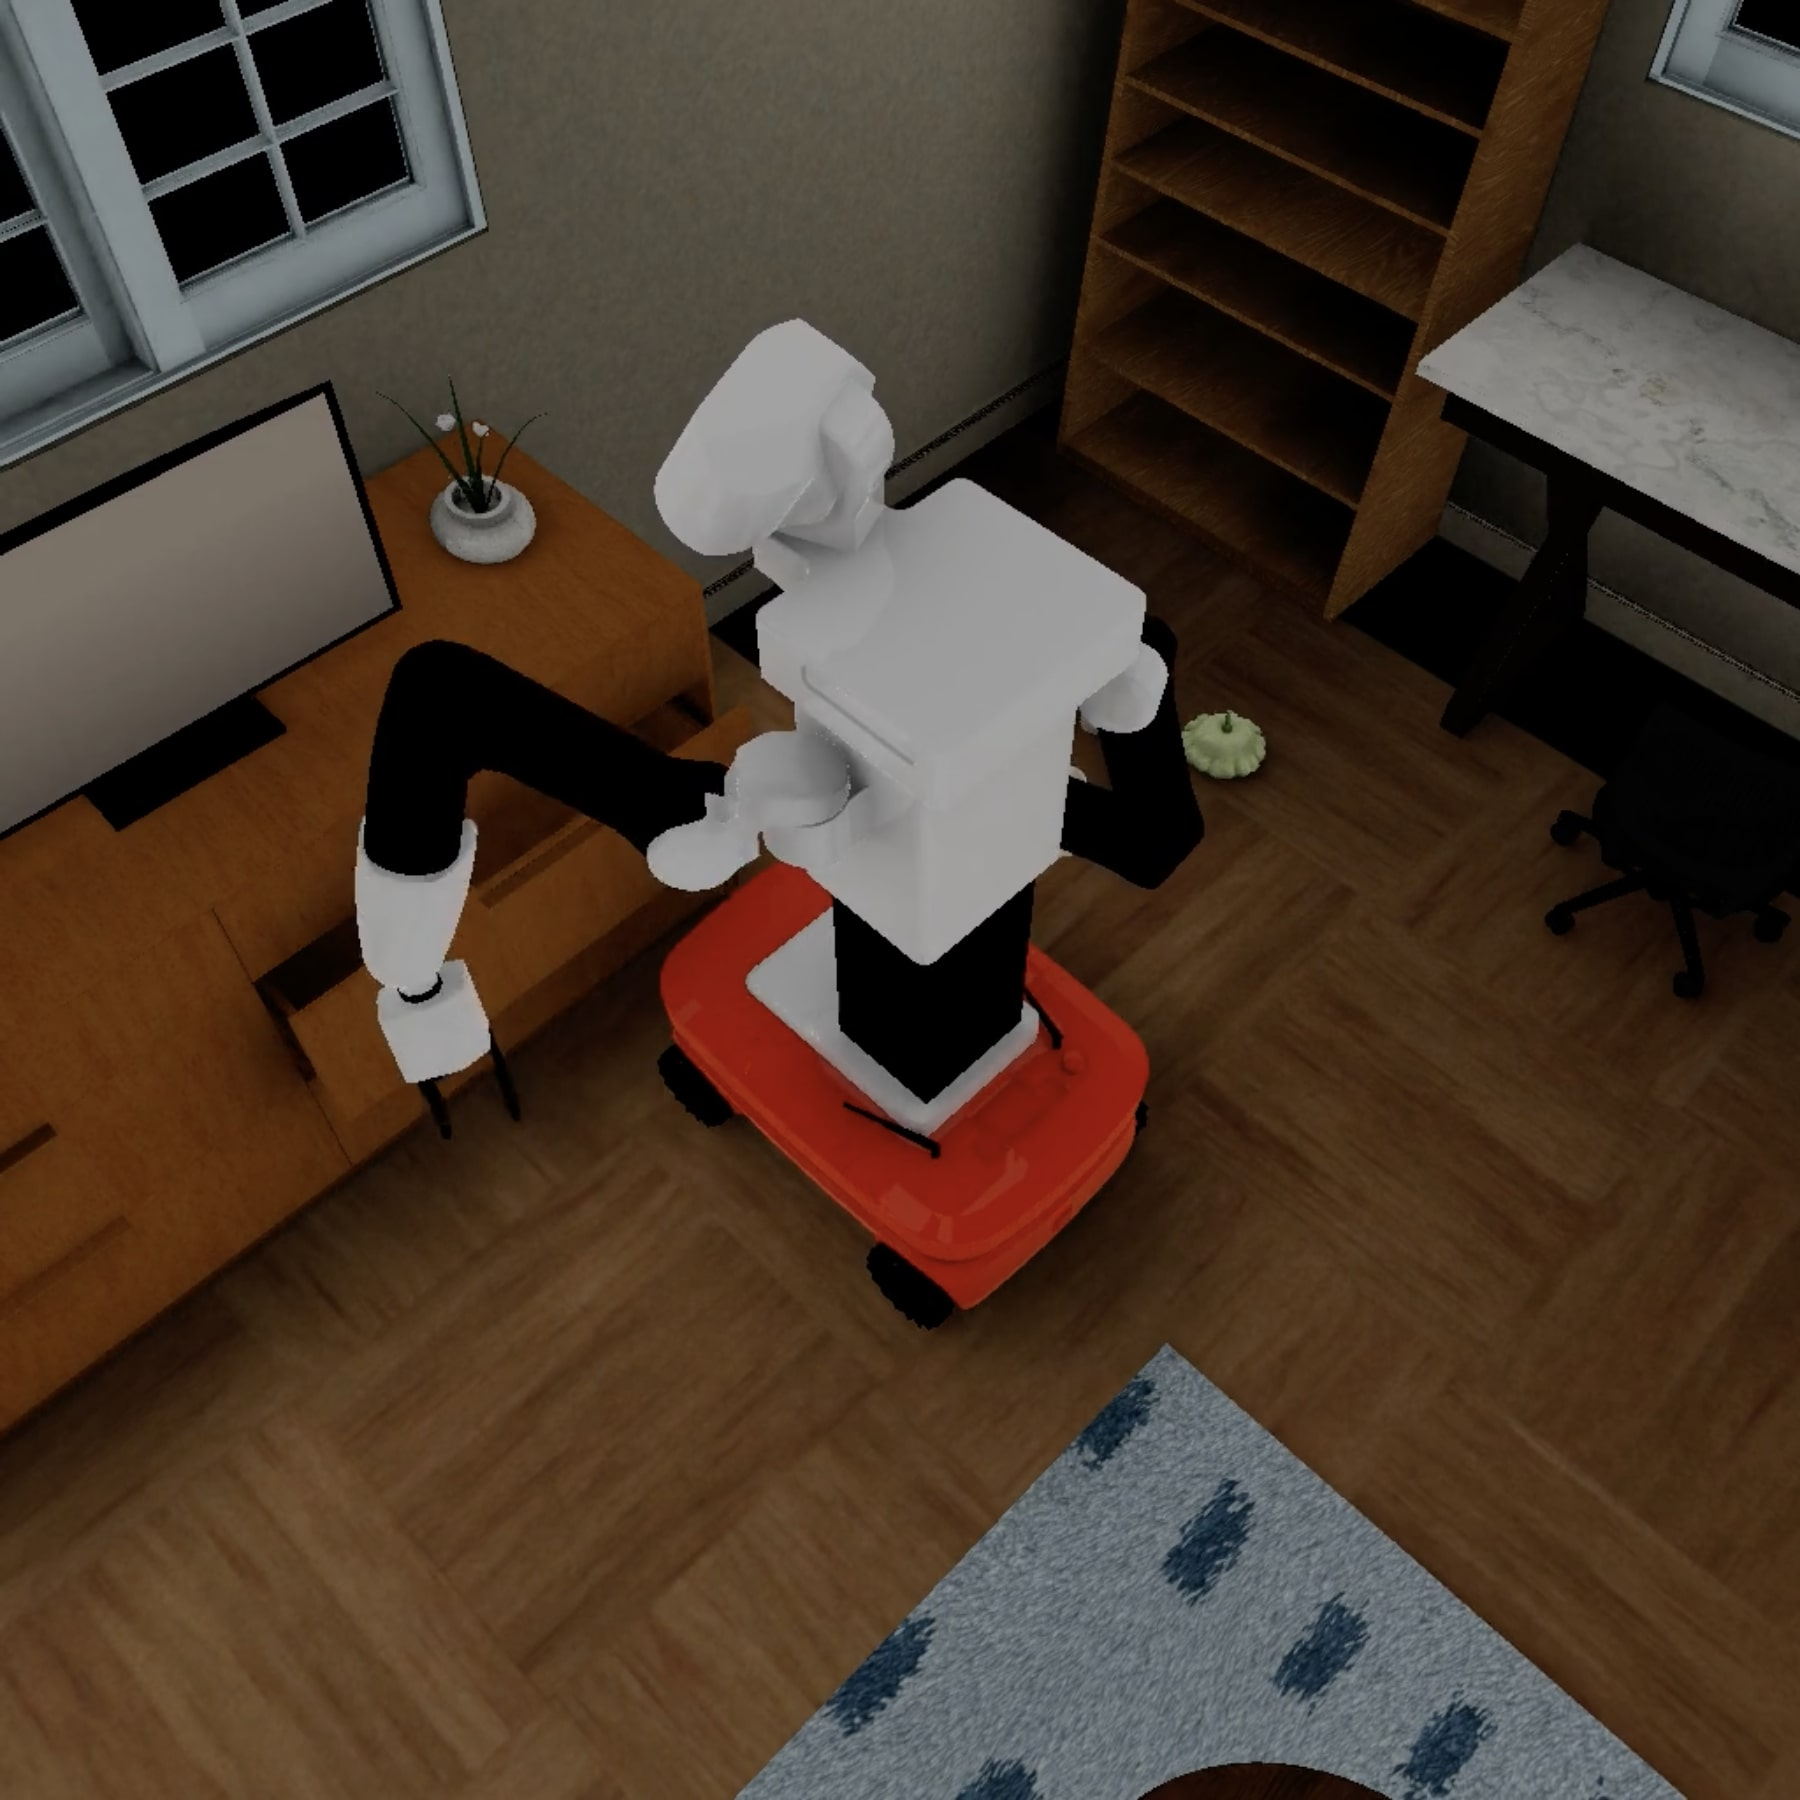
\includegraphics[width=0.3\linewidth]{figures/baseline_appendix/store_decoration_1.png}&
%         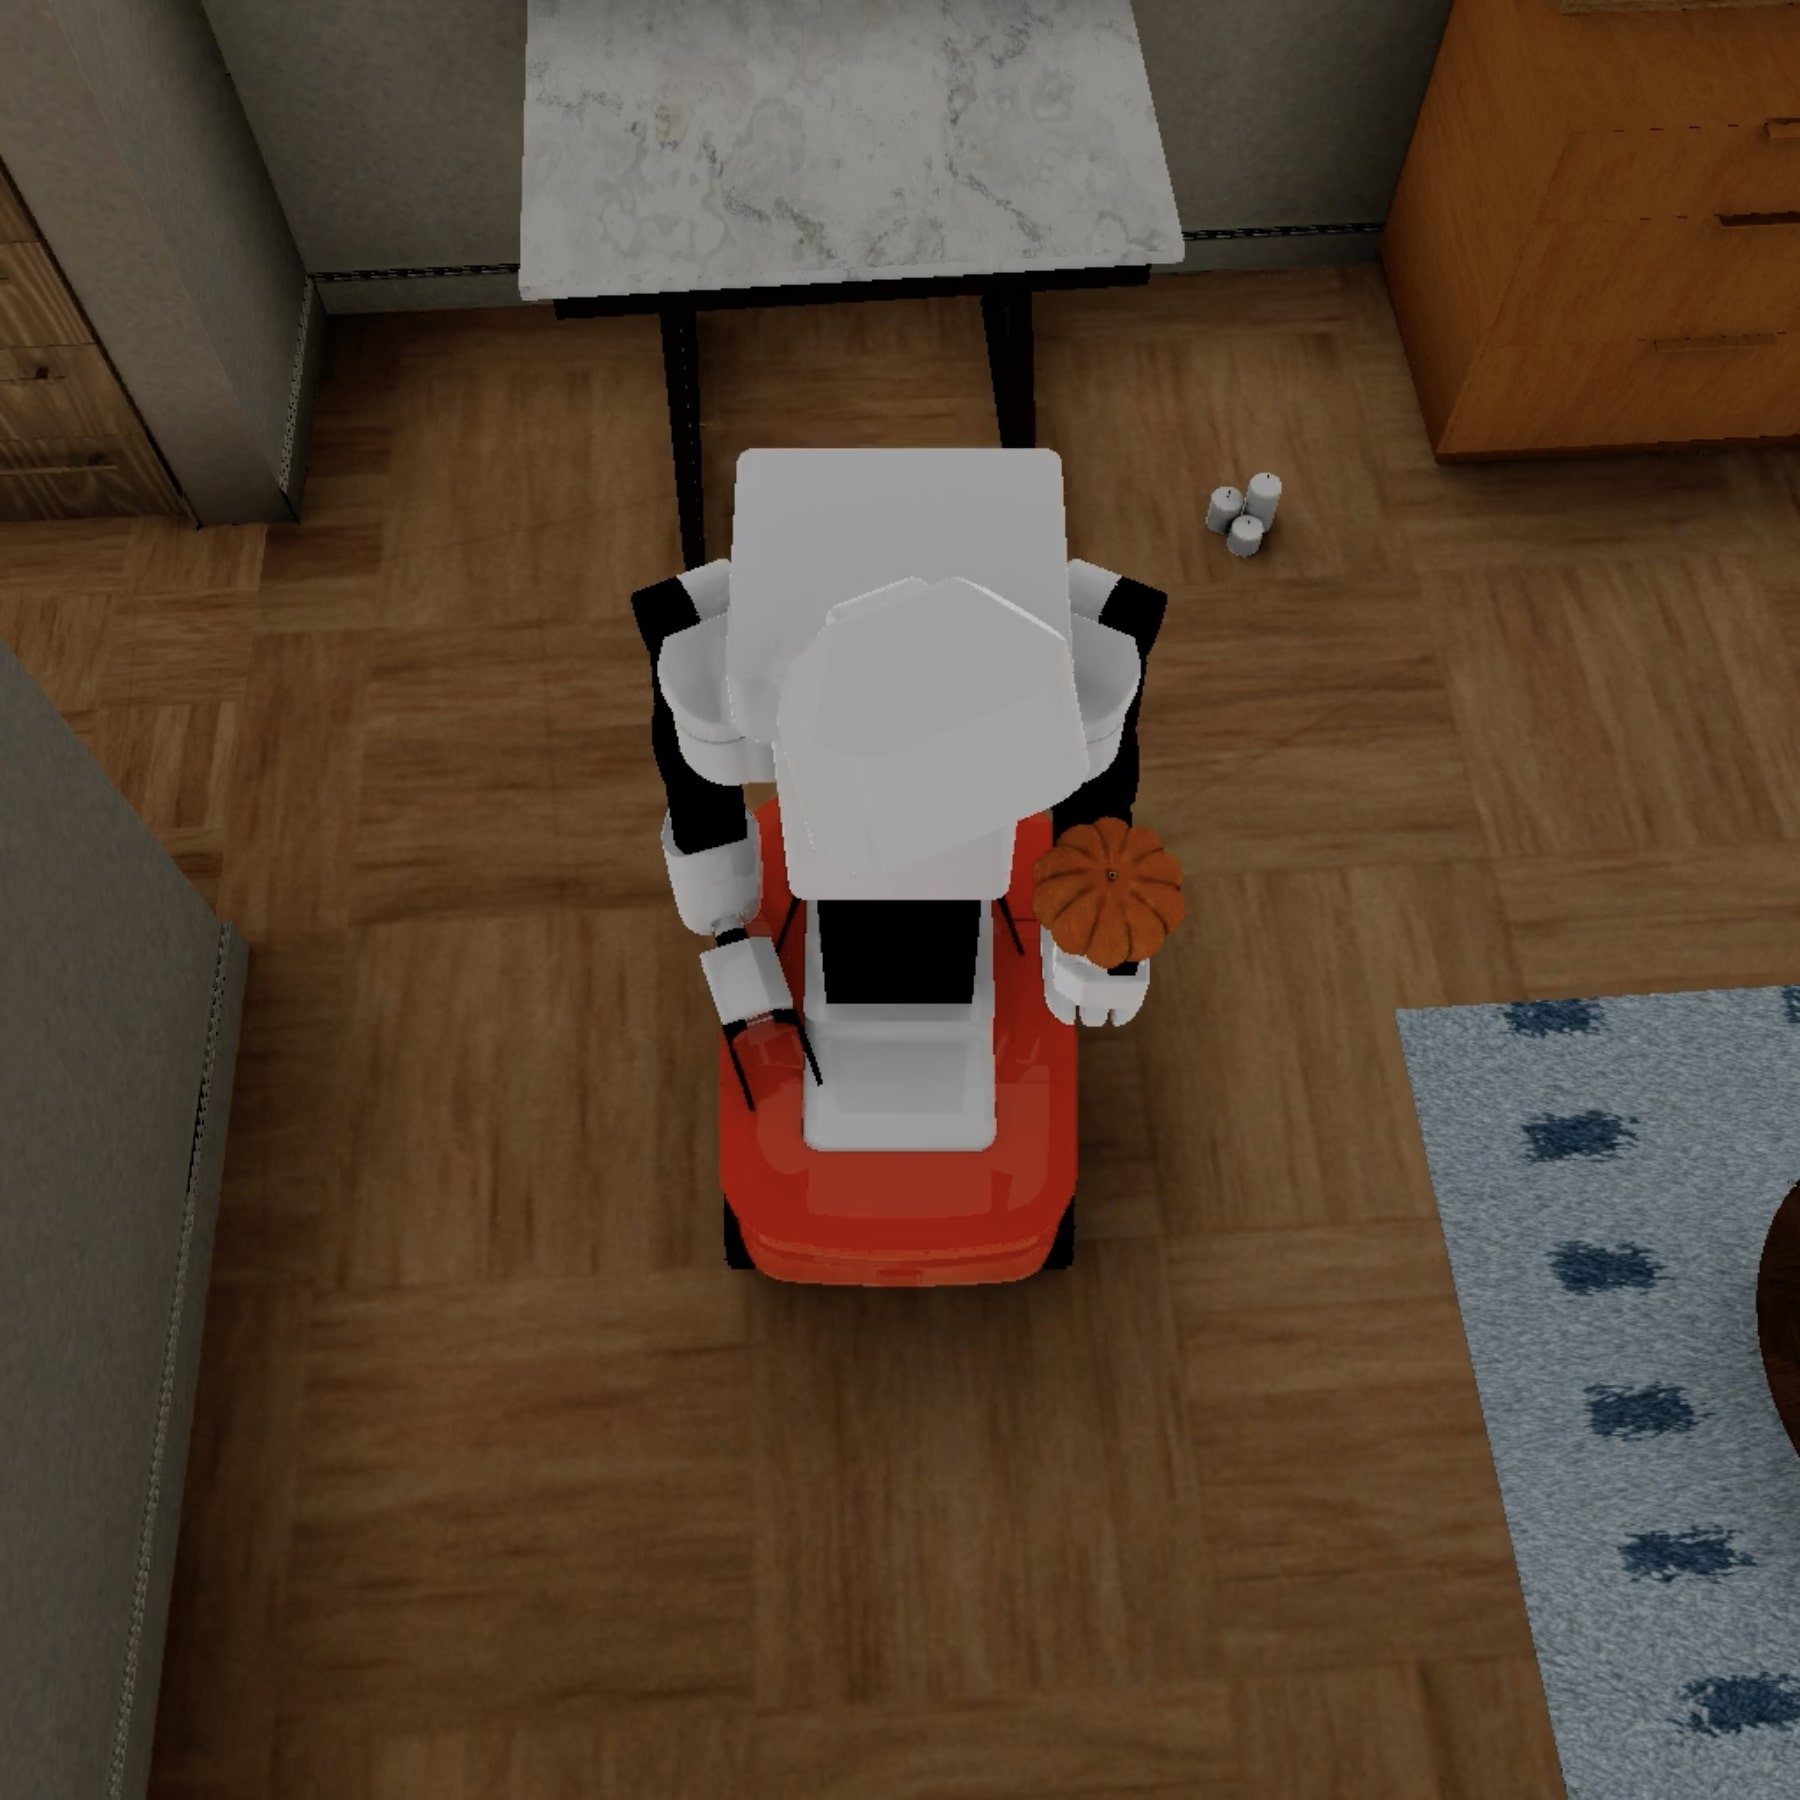
\includegraphics[width=0.3\linewidth]{figures/baseline_appendix/store_decoration_2.png}&
%         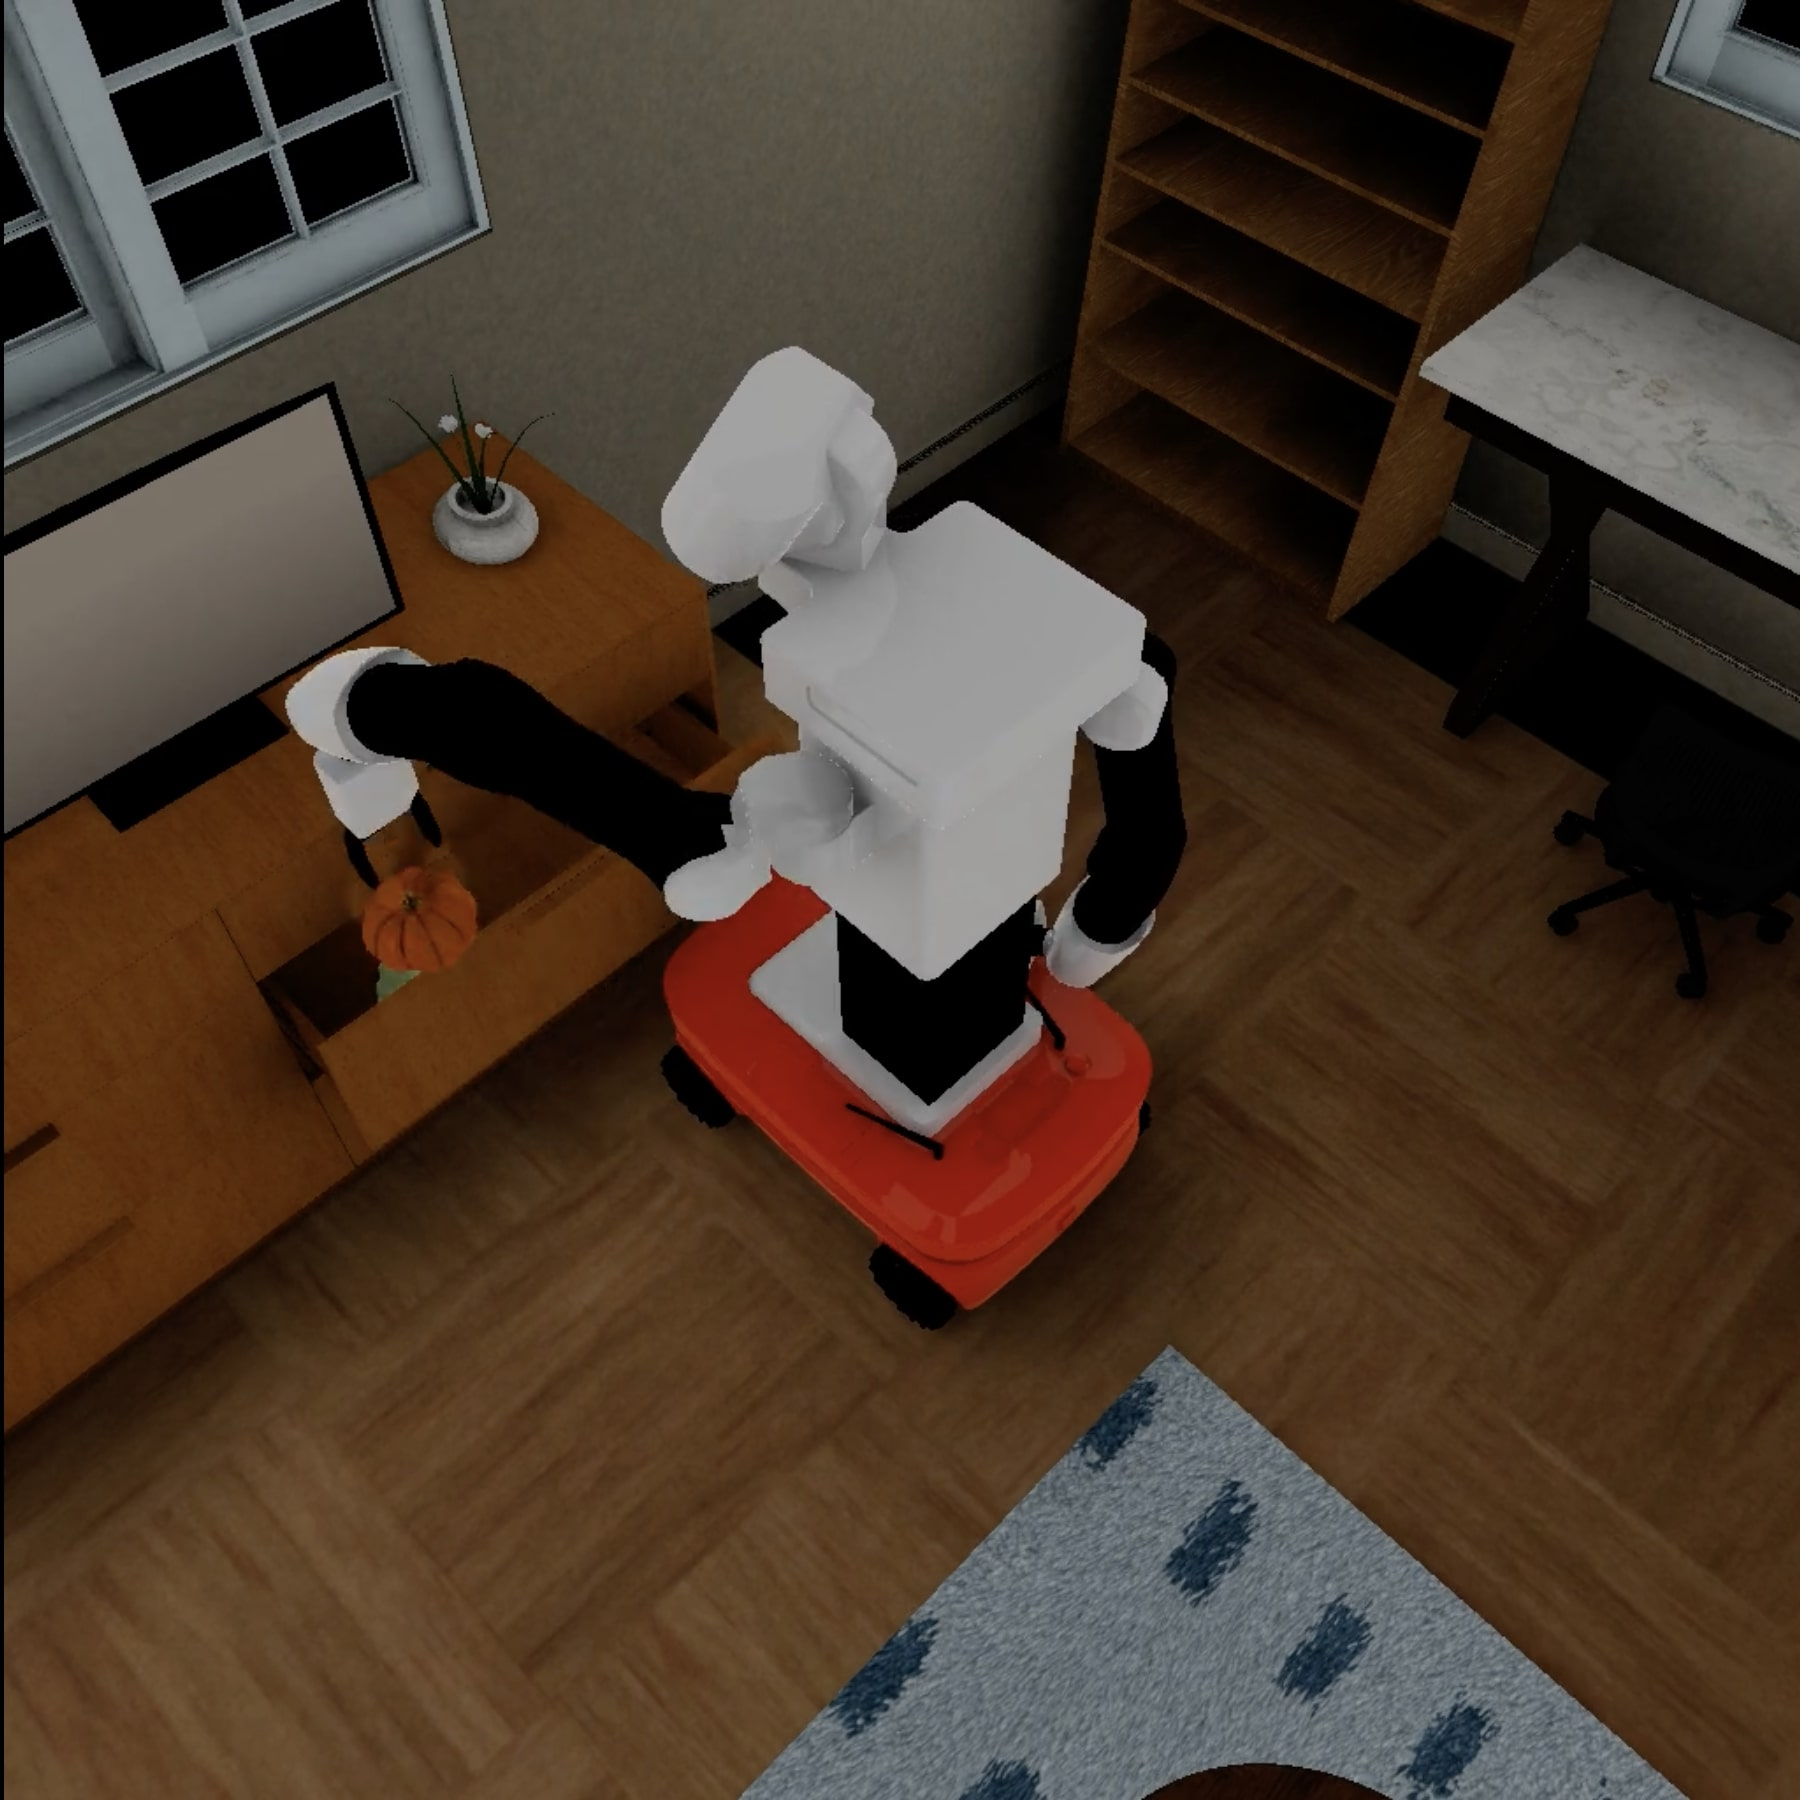
\includegraphics[width=0.3\linewidth]{figures/baseline_appendix/store_decoration_3.png}\\
%         & a) \texttt{StoreDecoration} & \\
%         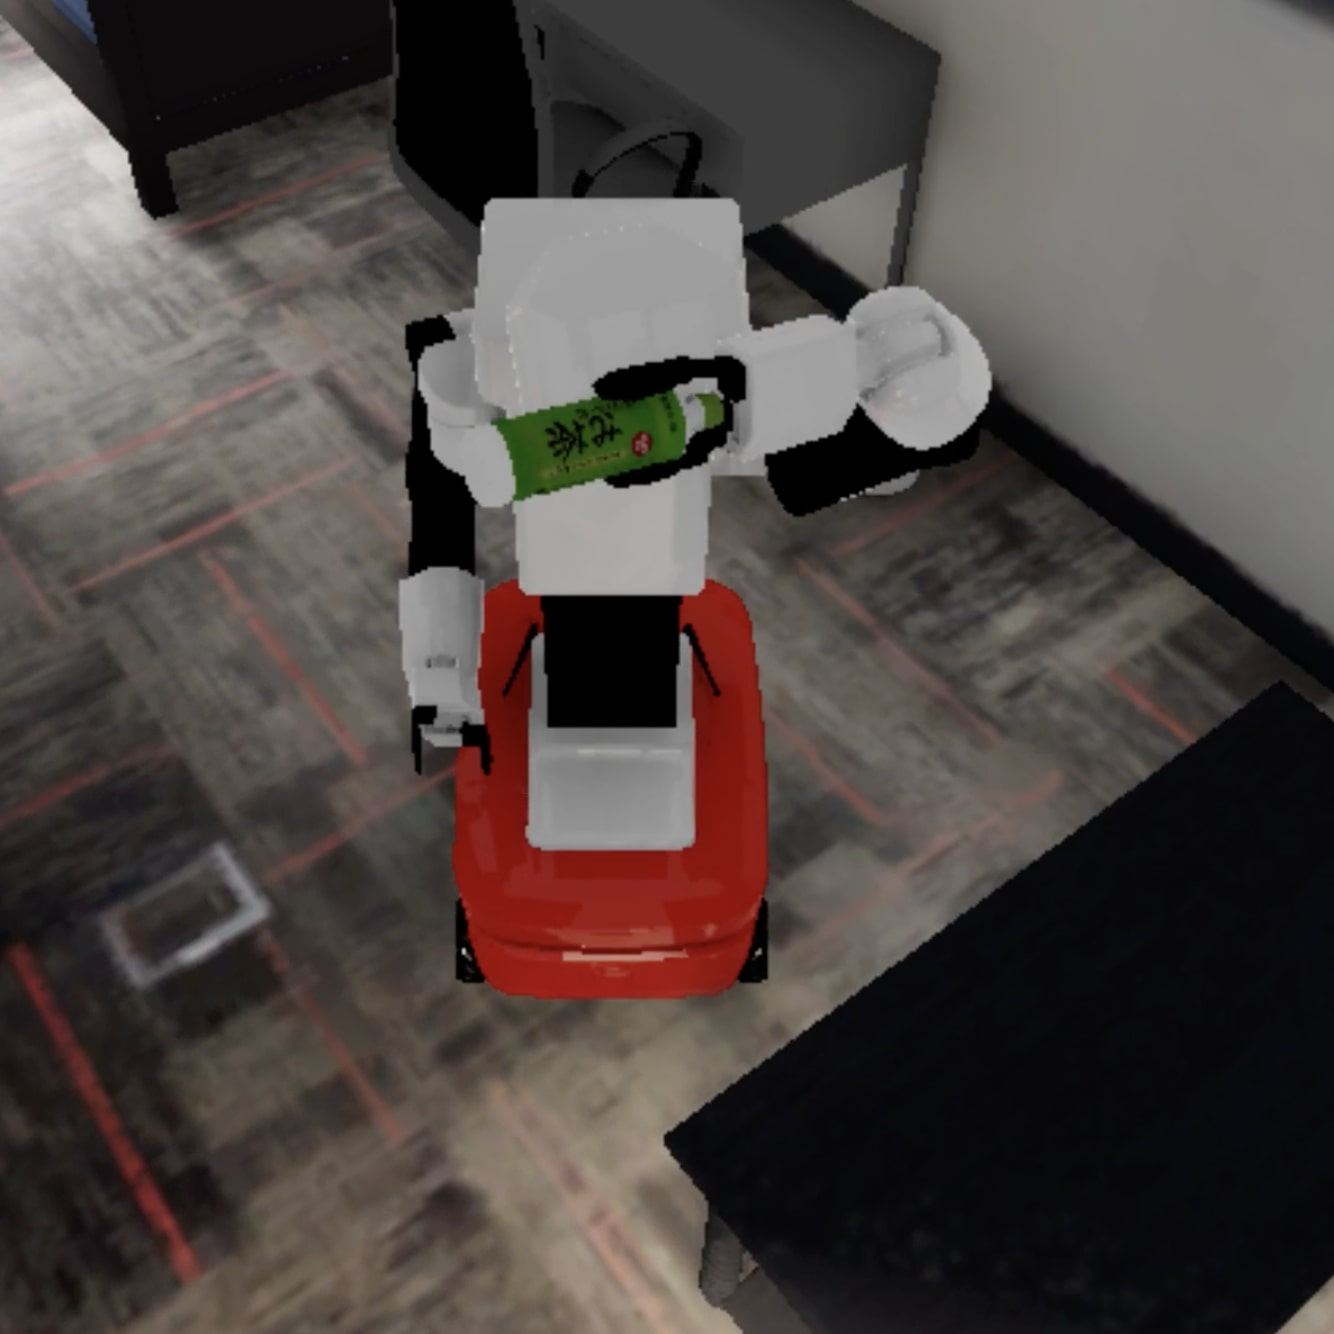
\includegraphics[width=0.3\linewidth]{figures/baseline_appendix/collect_trash_1.png}&
%         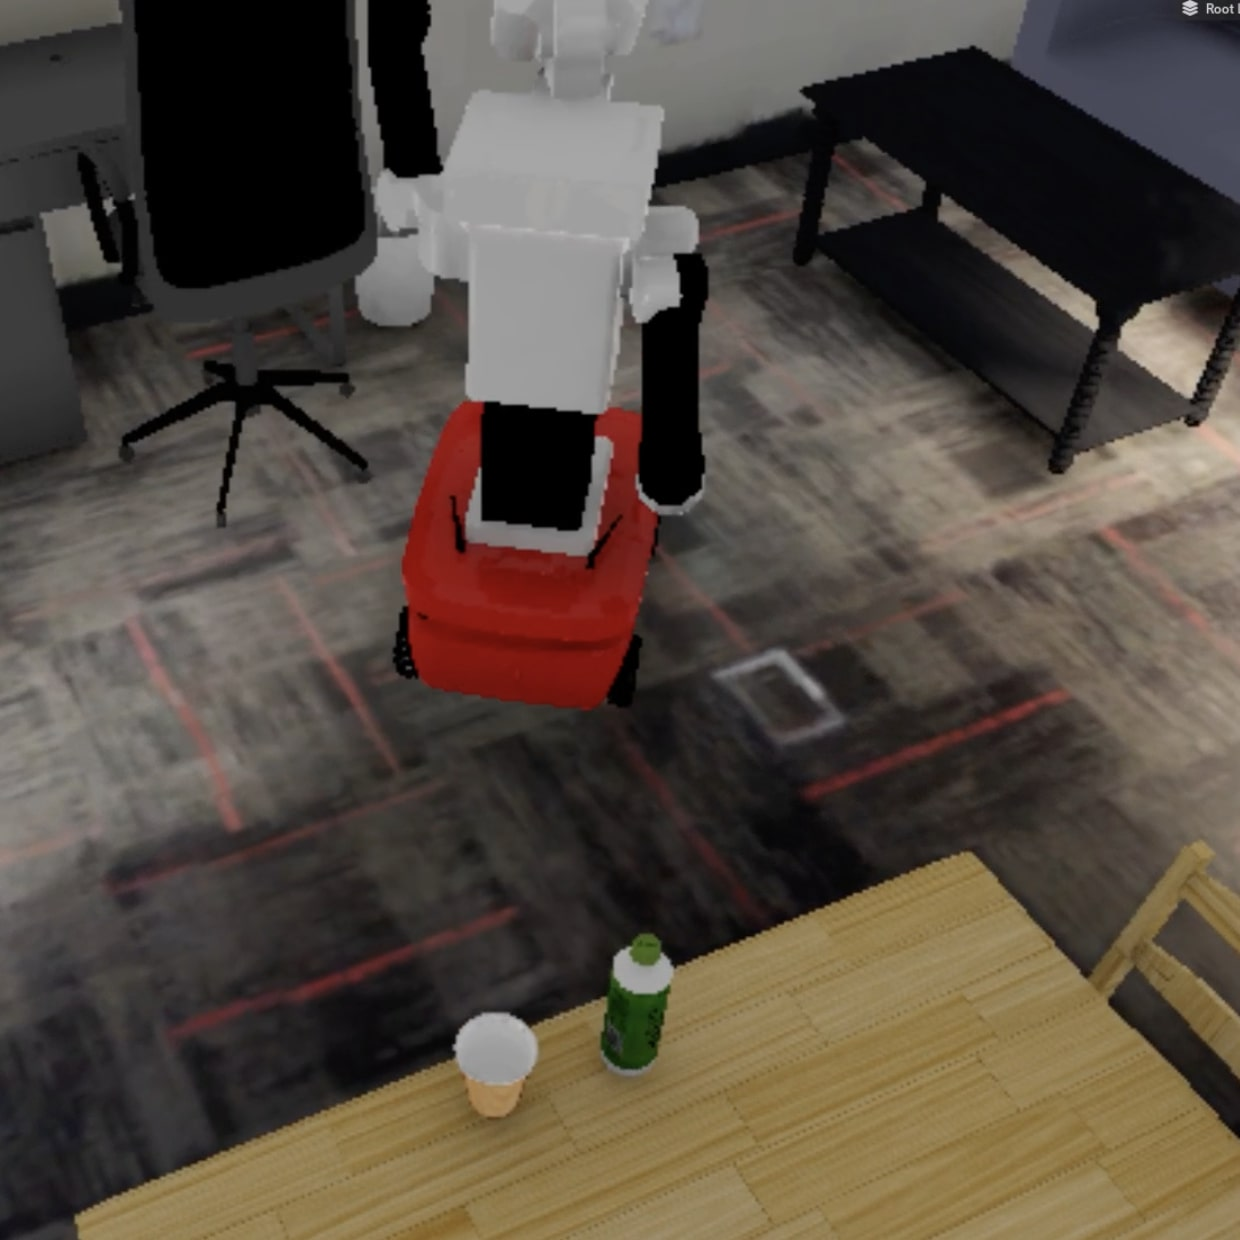
\includegraphics[width=0.3\linewidth]{figures/baseline_appendix/collect_trash_2.png}&
%         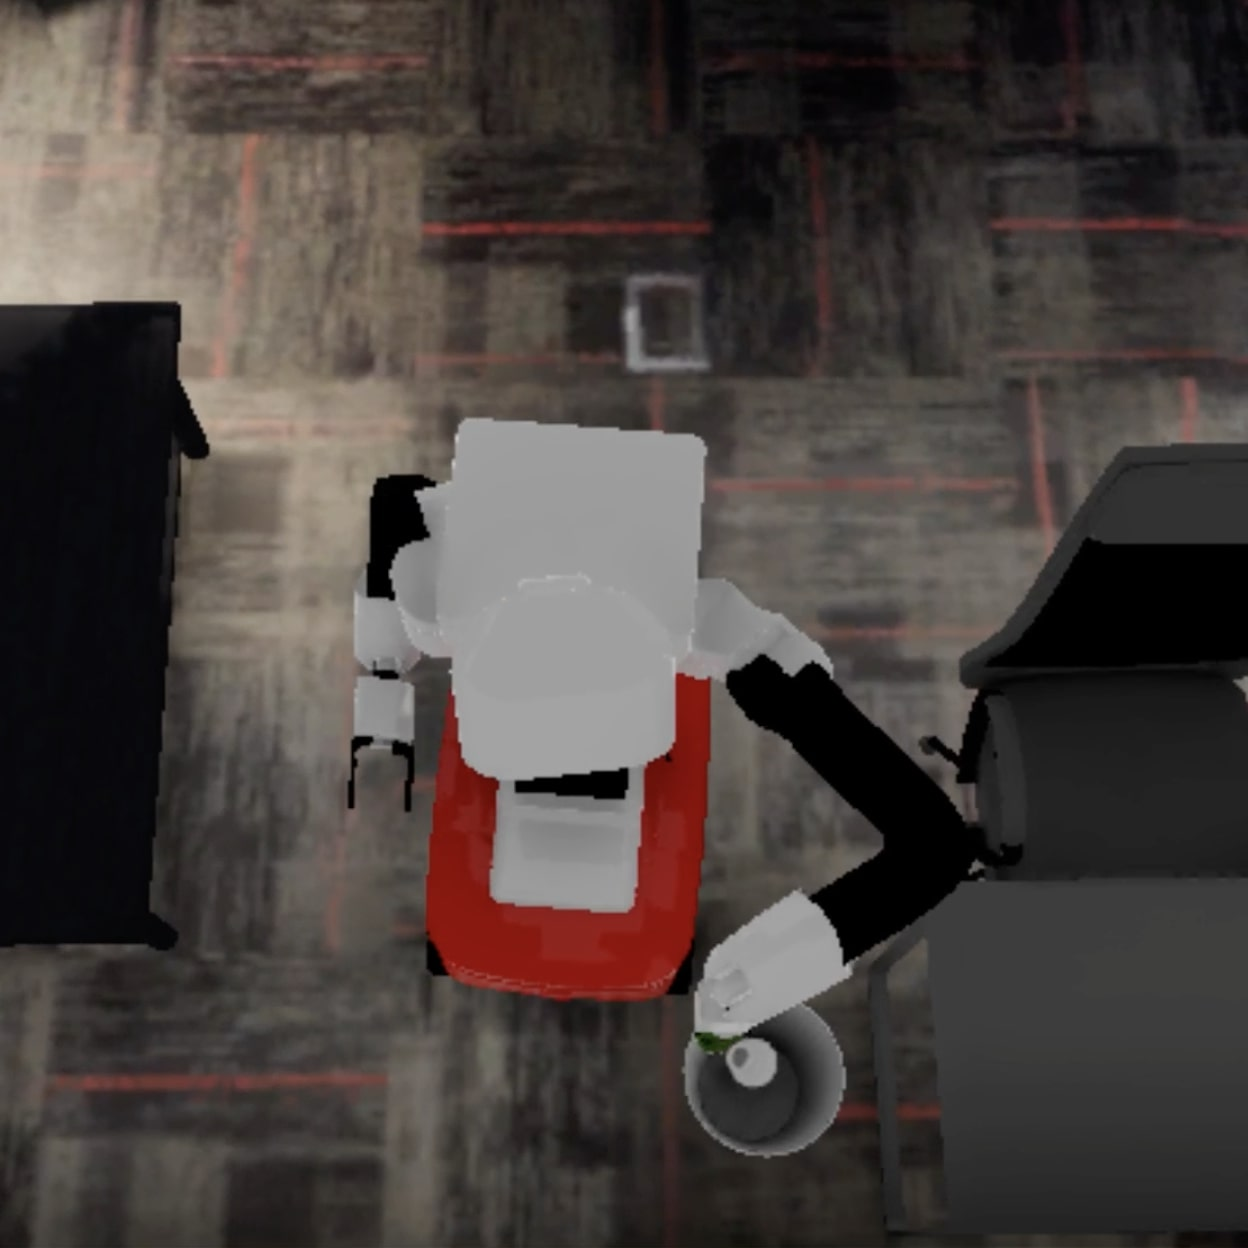
\includegraphics[width=0.3\linewidth]{figures/baseline_appendix/collect_trash_3.png}\\
%         & b) \texttt{CollectTrash} & \\
%         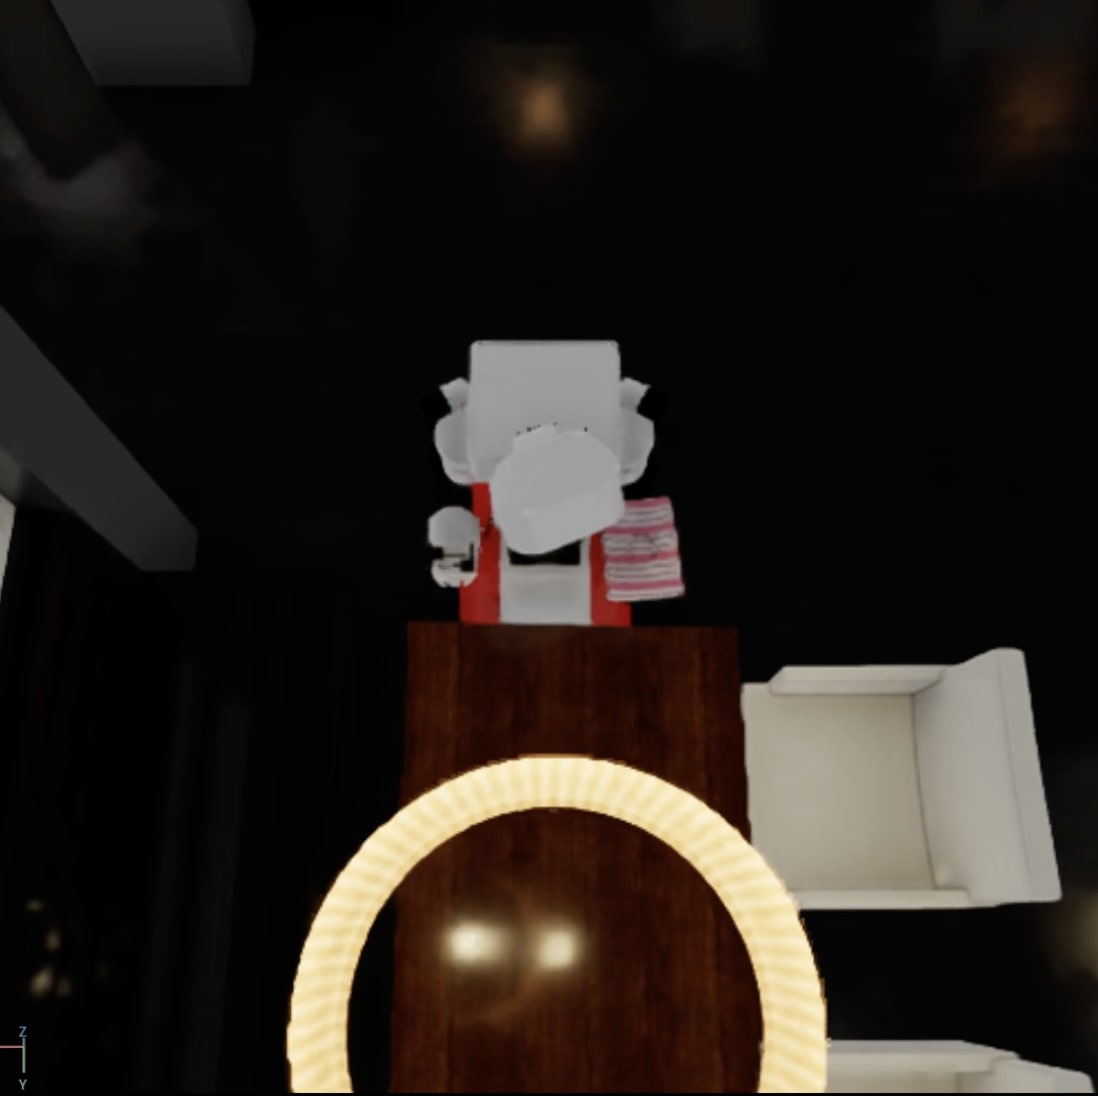
\includegraphics[width=0.3\linewidth]{figures/baseline_appendix/clean_table_1.png}&
%         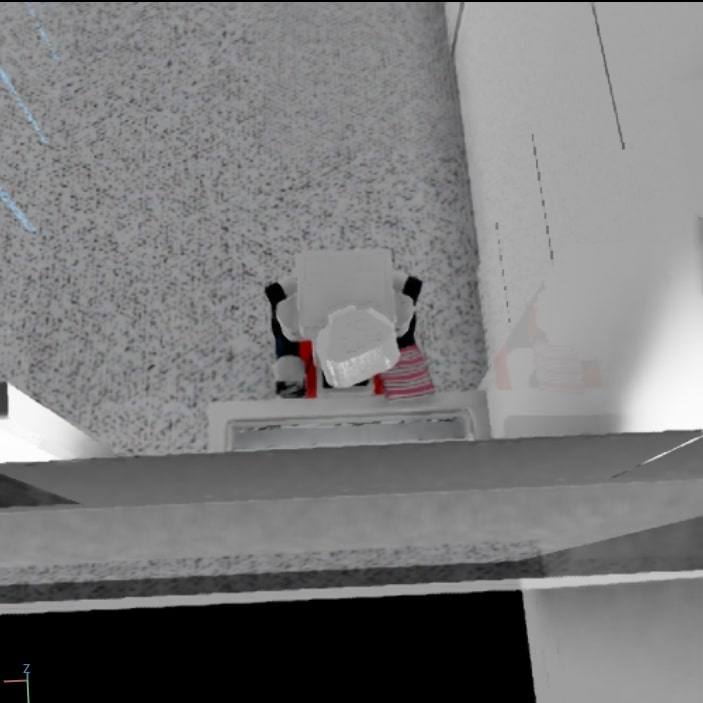
\includegraphics[width=0.3\linewidth]{figures/baseline_appendix/clean_table_2.png}&
%         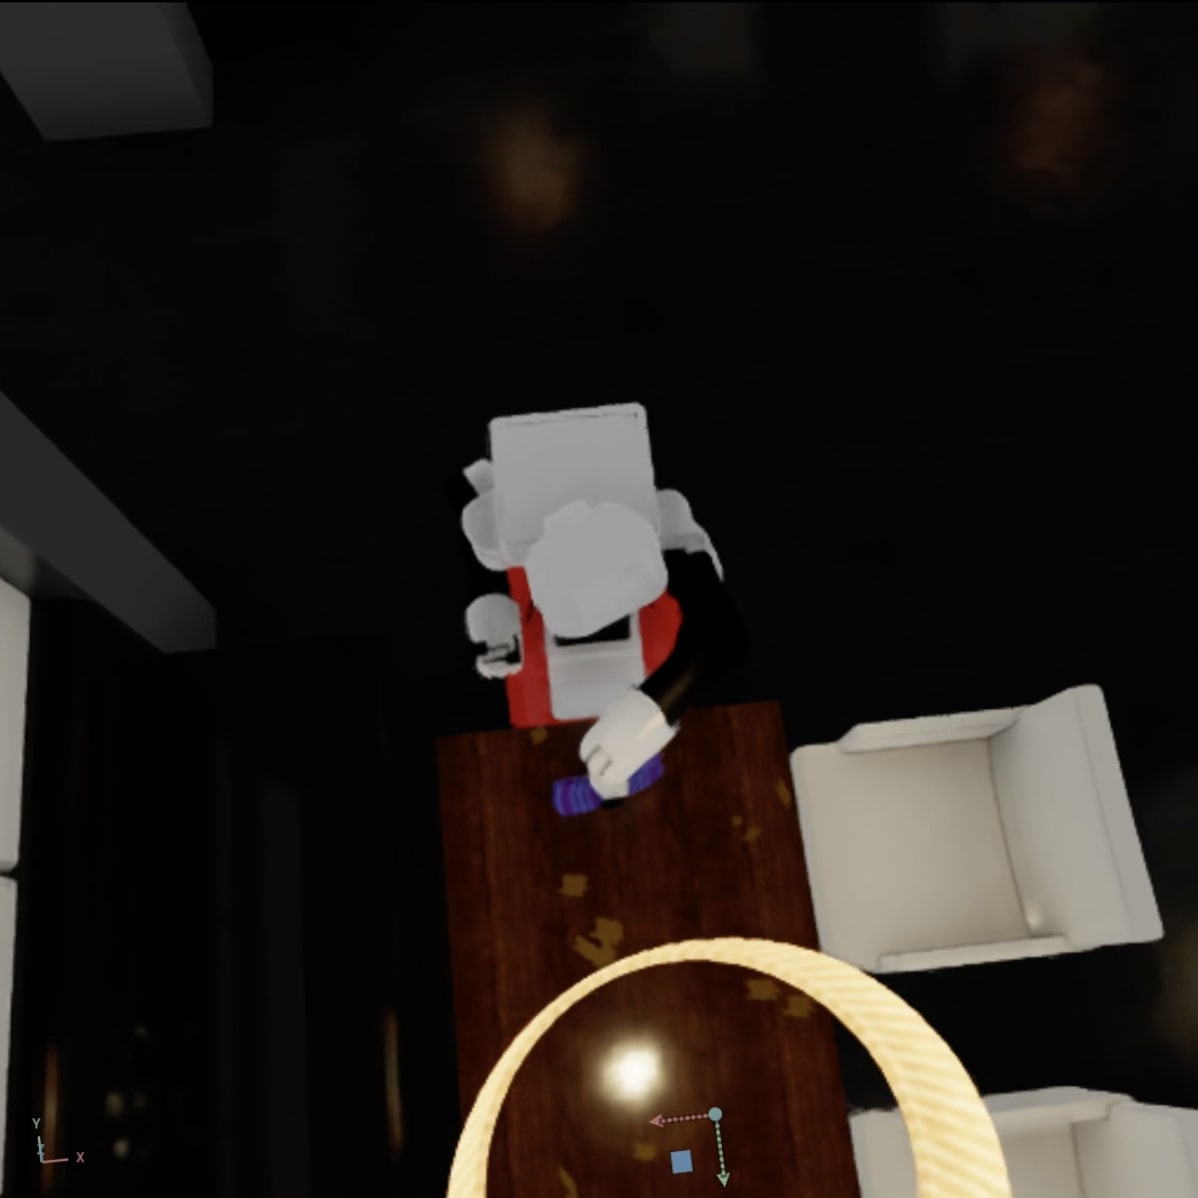
\includegraphics[width=0.3\linewidth]{figures/baseline_appendix/clean_table_3.png}\\
%         & c) \texttt{CleanTable} & \\
%     \end{tabular}
%     \caption{Overview of three tasks: \texttt{StoreDecoration}, \texttt{CollectTrash}, and \texttt{CleanTable}.}
%     \label{fig:appendix_task}
% \end{minipage}
% \end{figure*}


\subsection{Training details}

\paragraph{Learning objectives.} %\todo{Learning objectives for VMC} 
For \rlprim and \rlprimhist, we use an on-policy reinforcement learning algorithm Proximal Policy Optimization (PPO). $\theta$ is the policy parameter, $\hat{E}_t$ denotes the empirical expectation over timesteps. $r_{t}$ is the ratio of the probability under the new and old policies, respectively. $\hat{A}_t$ is the estimated advantage at time $t$. $\epsilon$ is the clipping hyperparameter. The objective function of PPO is shown in Equation~\ref{equ:ppo}:
\begin{equation}
    C^{CLIP}(\theta) = \hat{E}_t[\min r_t(\theta)\hat{A}_t, clip(r_t(\theta), 1-\epsilon, 1+\epsilon)\hat{A}_t].
    \label{equ:ppo}
\end{equation}
For \rlvmc, we use Soft Actor Critic (SAC) algorithm. The objective function is shown in Equation~\ref{equ:sac}:
\begin{equation}
    \pi^* = \arg\max_\pi E_{\tau\sim\pi}\left[\sum_{t=0}^\infty \gamma^t \left(R(s_t, a_t, s_{t+1})+\alpha H (\pi(\cdot|s_t)\right)\right],
    \label{equ:sac}
\end{equation}
where $\alpha$ is the coefficient that determines the weight of two terms and $H$ denotes the entropy.

\paragraph{Reward function.} %\todo{Reward for VMC, it should be the same as primitives baseline?} 
We use the success signal provided by the BDDL activity definition as the reward function for training the policy in all methods. For instance, in the \texttt{StoreDecorations} task, the BDDL task goal definition is \texttt{Forall(decoration)\{Inside(decoration, cabinet)\}}. The agent receive a positive signal if and only if one of the \texttt{decoration} is physically placed inside the \texttt{drawer} of the \texttt{cabinet}. This is a challenging sparse reward setting since the agent needs to plan multiple steps to reach the final goal without any intermediate subgoal rewards (e.g. \texttt{push} open the \texttt{drawer} must take place before \texttt{pick} and \texttt{place} the \texttt{decoration}, but no reward signal will be given to the \texttt{push} open action).% VMC uses the same reward function as other baselines.

\paragraph{Hyperparameters.} %\todo{Hyperparameters for VMC} 
The hyperparameters for SAC and PPO in the baselines are summarized in Table~\ref{tab:vmc_hyper_param} and Table~\ref{tab:ppo_hyper_param}. Both SAC and PPO are trained for 30,000 time steps. We train with seeds $0, 1, 2$ and evaluate with seed $0$.

\paragraph{Computation.}
\revision{For each run of our experiments, we use either a single Nvidia GeForce RTX 2080 Ti or a single Nvidia RTX A-6000 GPU, together with Intel Xeon CPU, and 40GB of RAM. During training, the GPU memory usage is around 9GB. Depending on which task, the total training iterations range between 10k to 25k, and the total wall-clock training time range between 3.75 to 7.5 hours.}

\begin{table}[t]
\centering
\begin{minipage}[t]{.41\linewidth}%
    \begin{tabular}{c|c}
    \toprule
        Learning Rate & $0.0003$ \\
        Buffer Size & $300$ \\
        Batch Size &  $64$ \\
        Discount ($\gamma$) & $0.99$ \\
        Soft Update Coefficient & $0.005$ \\
    \bottomrule
    \end{tabular}
    \caption{Hyperparameters of SAC for the \rlvmc baseline}
    \label{tab:vmc_hyper_param}
\end{minipage}
\hfill
\begin{minipage}[t]{.41\linewidth}%
    \begin{tabular}{c|c}
    \toprule
        Learning Rate & $0.0003$ \\
        Buffer Size & $300$ \\
        Batch Size &  $64$ \\
        Discount ($\gamma$) & $0.99$ \\
        GAE Parameter $\gamma_{gae}$ & $0.99$ \\
        Clipping Parameter $\epsilon$ & $0.2$ \\
        Entropy Coeff $c_1$ & $0.0$ \\
        VF Coeff $c_2$ & $0.5$ \\
    \bottomrule
    \end{tabular}
    \caption{Hyperparameters of PPO for the \rlprim and \rlprimhist baselines}
    \label{tab:ppo_hyper_param}
\end{minipage}
\end{table}

\subsection{Action Primitives} 
\benchmark activities are long-horizon which require hundreds if not thousands of environment steps (low-level robot control signals) to be completed.  A way to overcome this challenge (e.g., reinforcement learning) is to modify the original action space with a set of \textit{action primitives}, i.e., time-extended actions that correspond to multiple low-level commands and that achieve some expected outcome, such as grasping an object or navigating to a location. For our baselines, we defined six of these primitives, and implemented them using a sampling-based motion planner.

All the primitives are compositional: collision-free paths of the entire robot to navigate to a location, collision-free paths of the robot's arm to reach a \texttt{6D\_pose} with the end-effector, or a predefined arm joint configuration, trajectories where the end-effector follows a \texttt{line} in Cartesian space, possibly colliding/interacting with the environment, and sequences of actions to \texttt{open}/\texttt{close} the robot's gripper while holding the position.
All manipulation primitives start with a trajectory to move the arm from a tucked configuration (folded arm) to an untucked configuration to enable subsequent arm interaction, and end with the inverse motion, from untucked to tucked configuration, to allow subsequent collision-free navigation.
The action primitives take as parameter an object to apply the action on; we assume access to the 3D position of the objects to obtain the necessary parameters to query the motion planner. This procedure is replicated on the real robot, where we combine detections from YOLO~\cite{redmon2018yolov3} with information from the depth map of the RGB-D images to obtain the parameters (see Sec.~\ref{as:s2r}). For the navigation actions, we assume a set of known relevant locations to navigate to (next to the rectangles in Fig.~\ref{fig:baseline_task}) 

The primitives we used in our experiments can be seen in Fig.~\ref{fig:appendix_high_level_planner} and include:
\vspace{-2mm}
\begin{itemize}[leftmargin=2em]
\item[a)] \texttt{navigate}: Collision-free trajectory of the entire robot to a location.
\item[b)] \texttt{pick}: Composition of 1) a trajectory to a pre-grasp \texttt{6D\_pose} above the object to pick, 2) a \texttt{line} trajectory in Cartesian space down towards the object, interrupted when there is contact, 3) a \texttt{closing} action, 4) a first retracting trajectory following a \texttt{line} upwards, and 5) a second retracting trajectory to reach the untucked joint configuration. The primitive only executes if the robot is not currently picking another object.
\item[c)] \texttt{place}: Composition of 1) a trajectory to a pre-place \texttt{6D\_pose} above the object to place the grasped object on, 2) an \texttt{opening} action, 3) a second retracting trajectory to reach the untucked joint configuration. The primitive only executes if the robot is currently holding an object.
\item[d)] \texttt{push}: Composition of 1) a trajectory to a pre-push \texttt{6D\_pose} above the object to push-open, 2) a \texttt{line} trajectory in Cartesian space down towards the object, interrupted if there is contact, 3) a \texttt{line} trajectory in Cartesian space to push-open the object, e.g., towards the robot, 4) a first retracting trajectory following a \texttt{line} upwards, and 5) a second retracting trajectory to reach the untucked joint configuration. 
\item[e)] \texttt{dip}: Composition of 1) a trajectory to a pre-dip \texttt{6D\_pose} above the object to dip into, 2) a \texttt{line} trajectory in Cartesian space down towards the object to dip, 3) a \texttt{line} trajectory in Cartesian space upwards, and 4) a retracting trajectory to reach the initial joint configuration. The primitive only executes if the robot is currently holding an object.
\item[f)] \texttt{wipe}: Composition of 1) a trajectory to a pre-wipe \texttt{6D\_pose} above the object to wipe, 2) a \texttt{line} trajectory in Cartesian space down towards the object to be wiped, interrupted when there is contact, 3) a \texttt{line} trajectory in Cartesian space horizontally to wipe left-right, 4) a \texttt{line} trajectory in Cartesian space horizontally to wipe towards the robot, 4) a first retracting trajectory following a \texttt{line} upwards, and 5) a second retracting trajectory to reach the untucked joint configuration. The primitive only executes if the robot is currently holding an object.
\end{itemize}

% \begin{figure}[h!]
% \centering
%     \renewcommand\tabcolsep{0.5pt}
%     \begin{tabular}{ccc}        
%         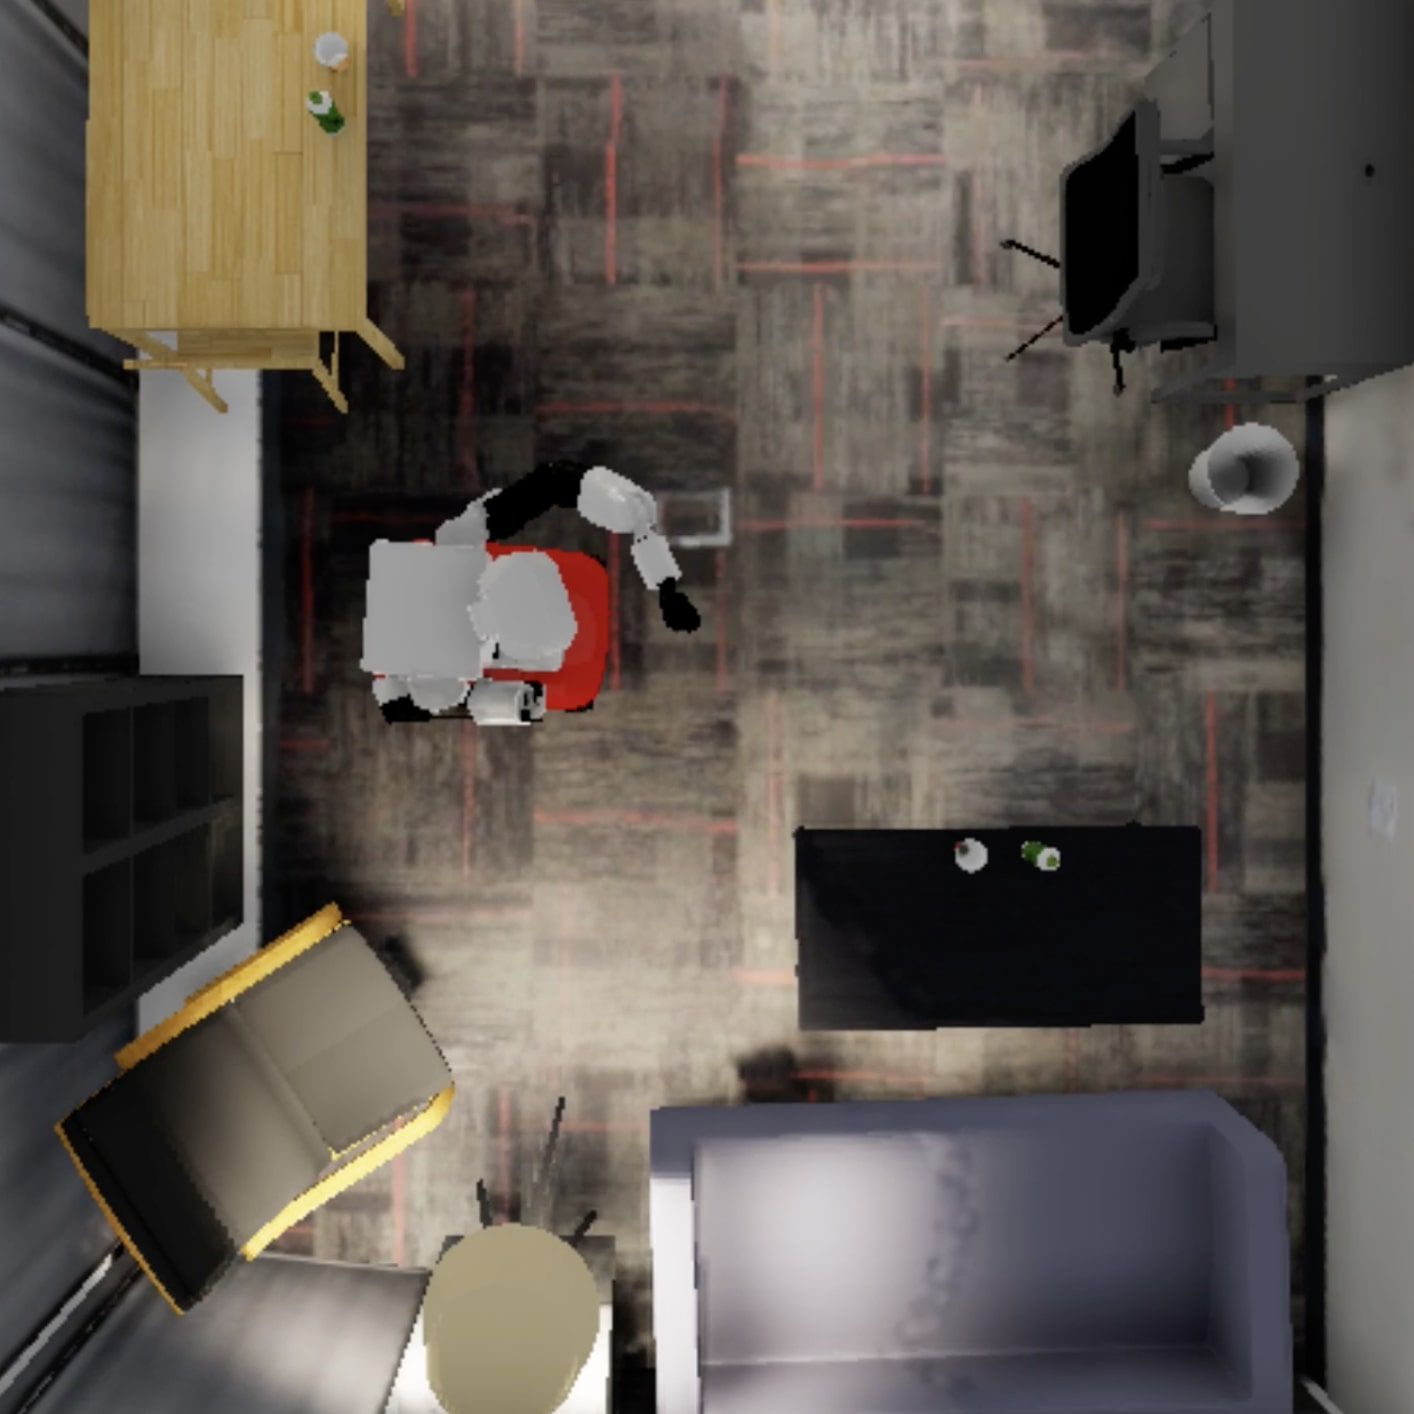
\includegraphics[trim=0 200 0 200,clip,width=0.3\linewidth]{figures/baseline_appendix/navigate_to_1}&
%         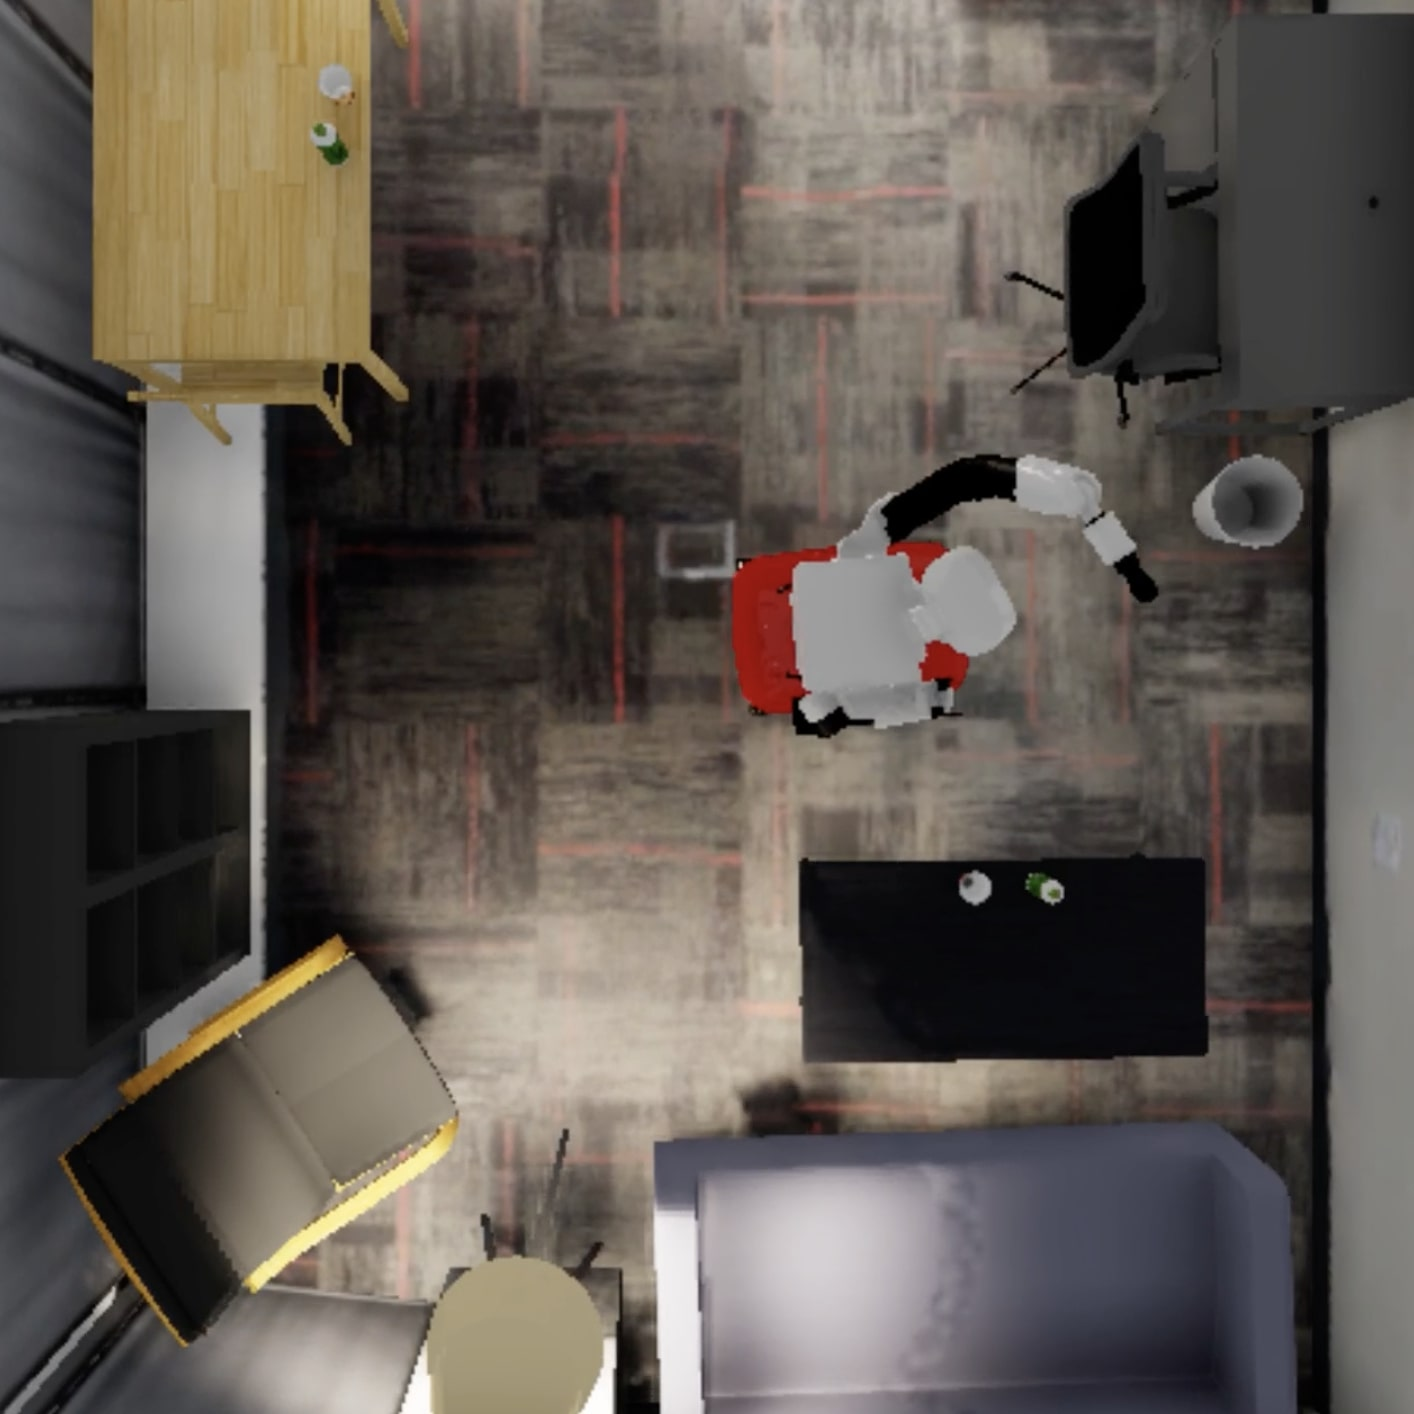
\includegraphics[trim=0 200 0 200,clip,width=0.3\linewidth]{figures/baseline_appendix/navigate_to_2}&
%         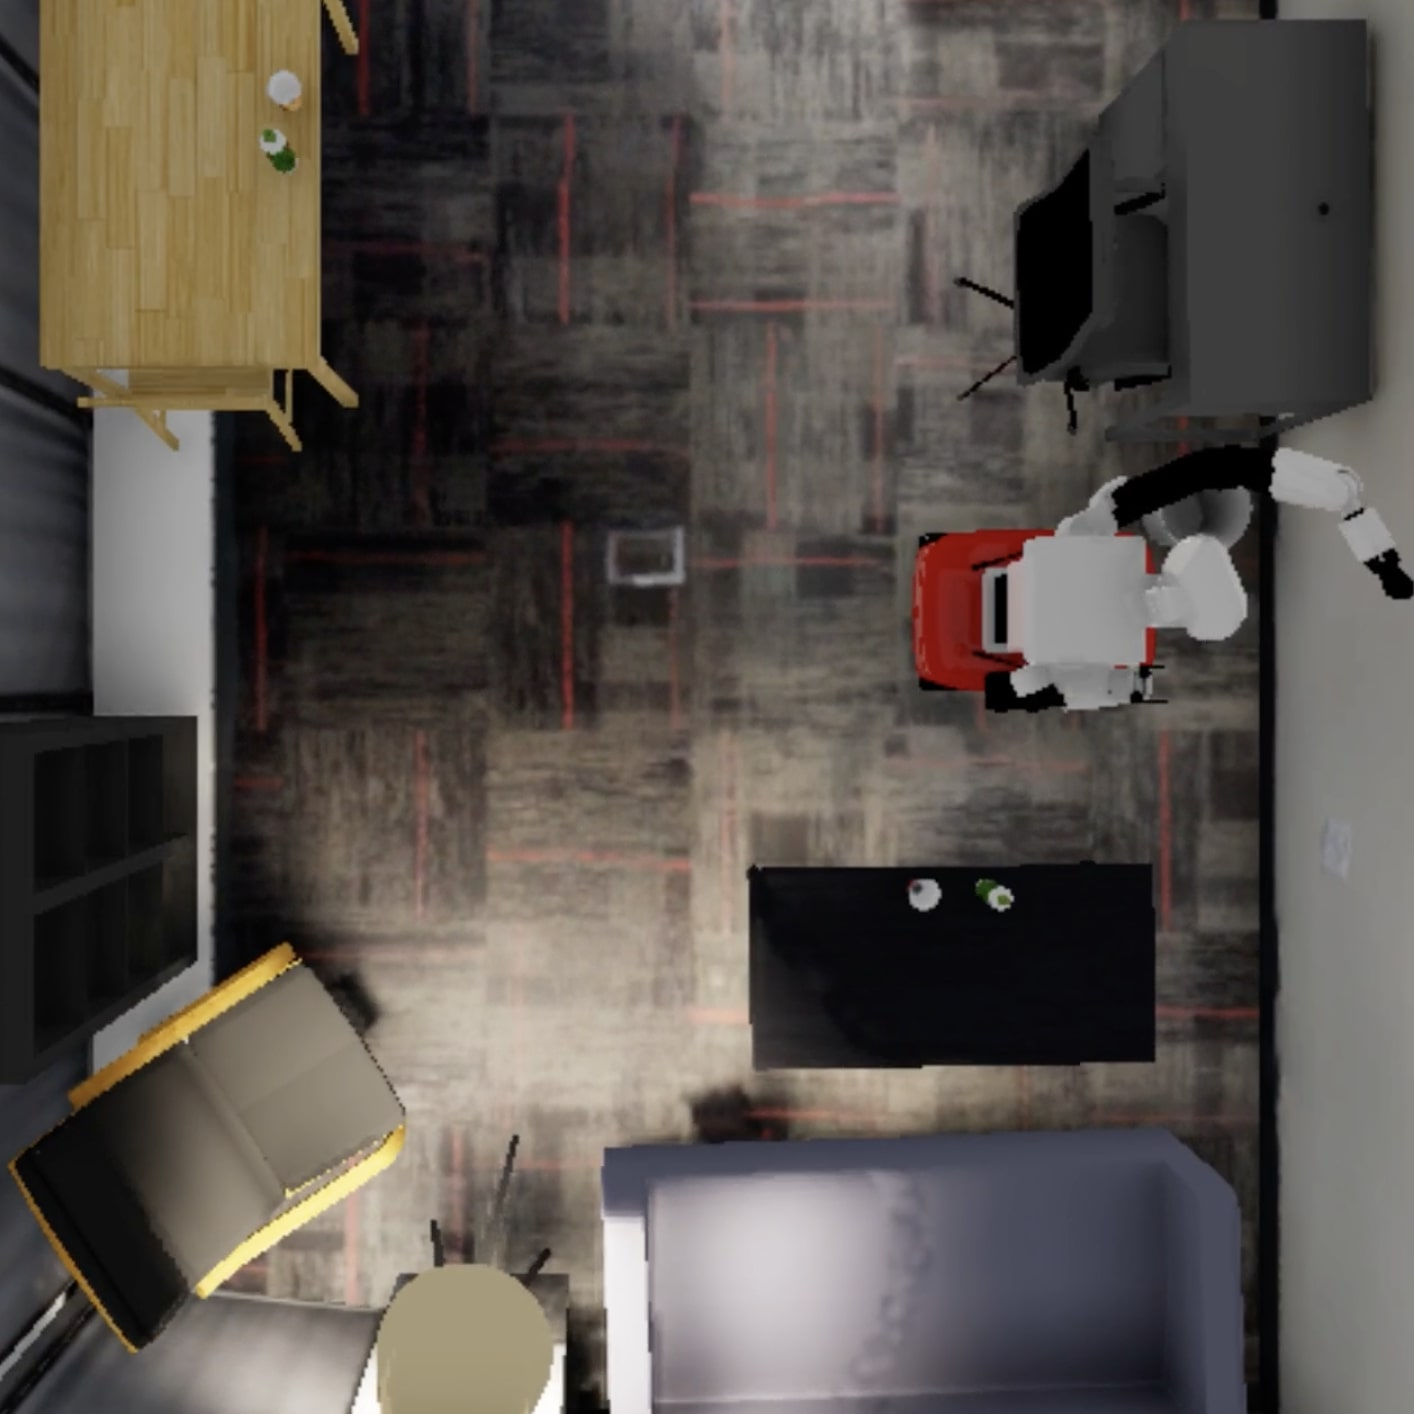
\includegraphics[trim=0 200 0 200,clip,width=0.3\linewidth]{figures/baseline_appendix/navigate_to_3}\\
%         & a) \texttt{navigate} & \\
%         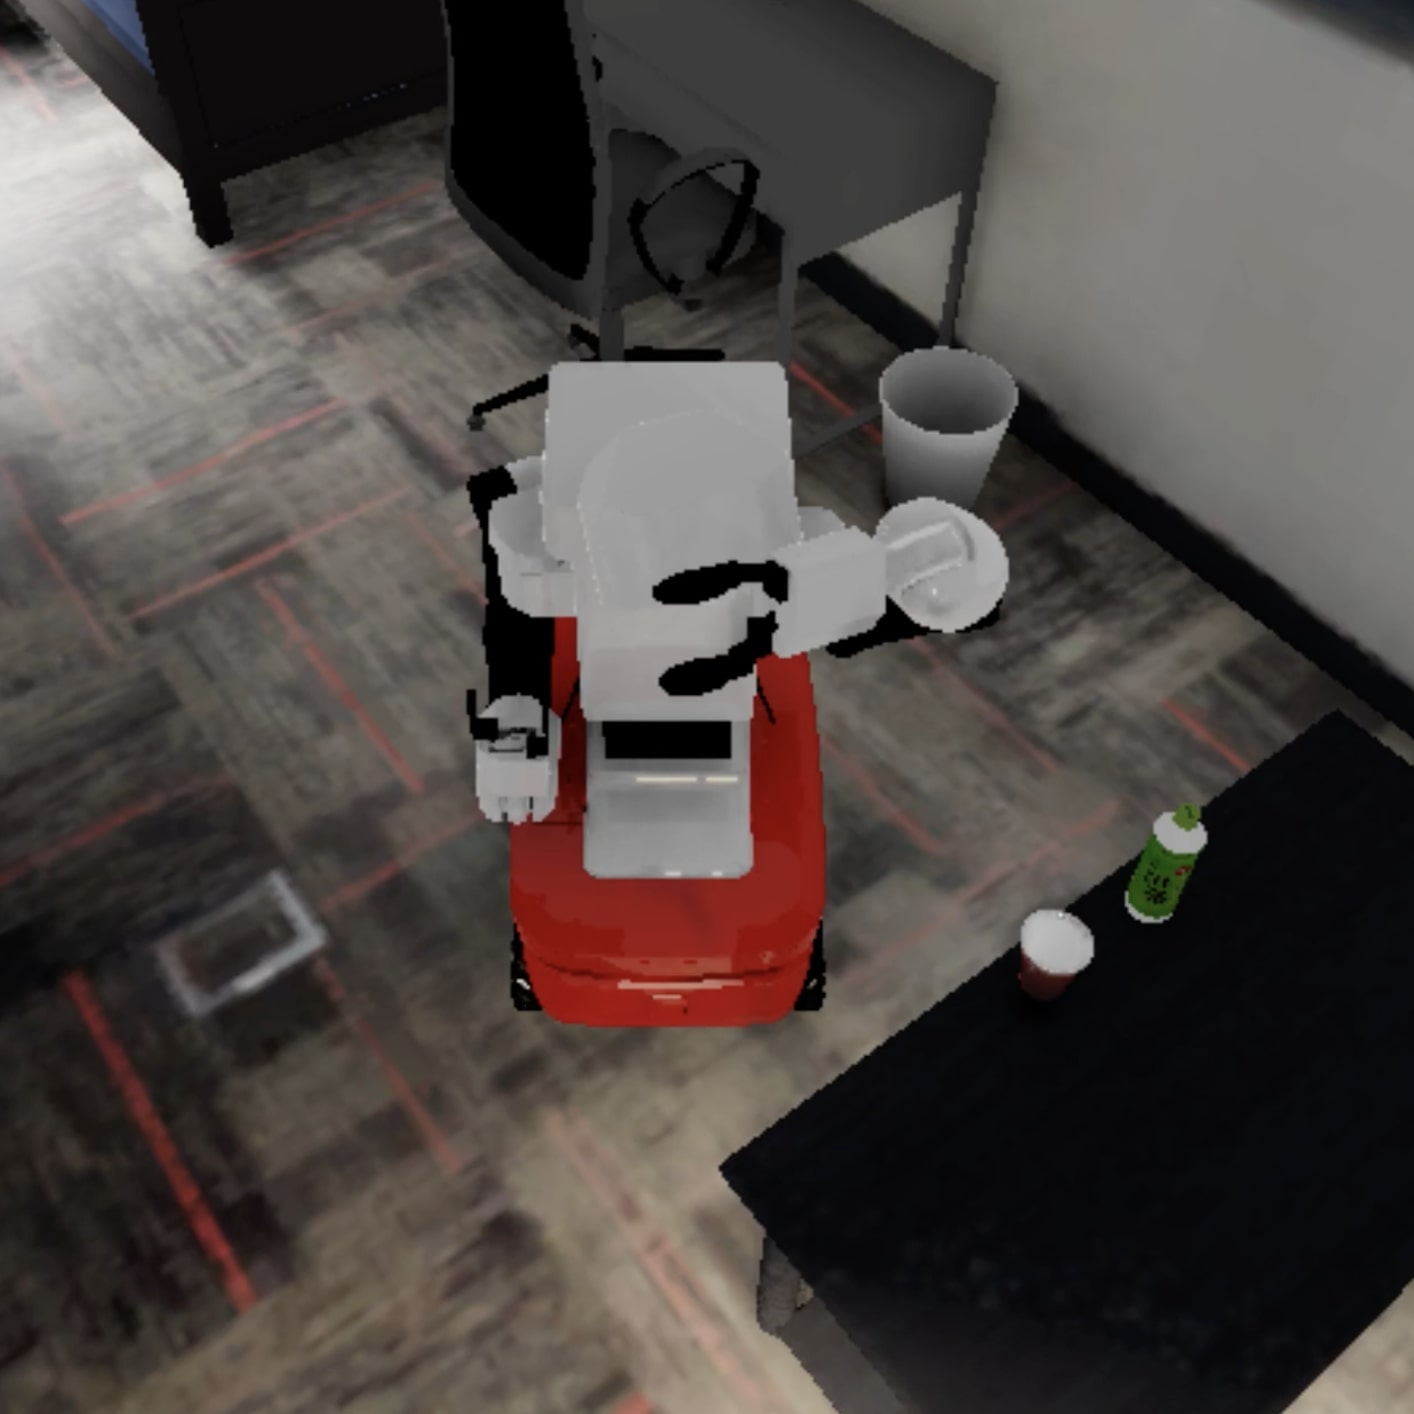
\includegraphics[trim=0 200 0 200,clip,width=0.3\linewidth]{figures/baseline_appendix/pick_1}&
%         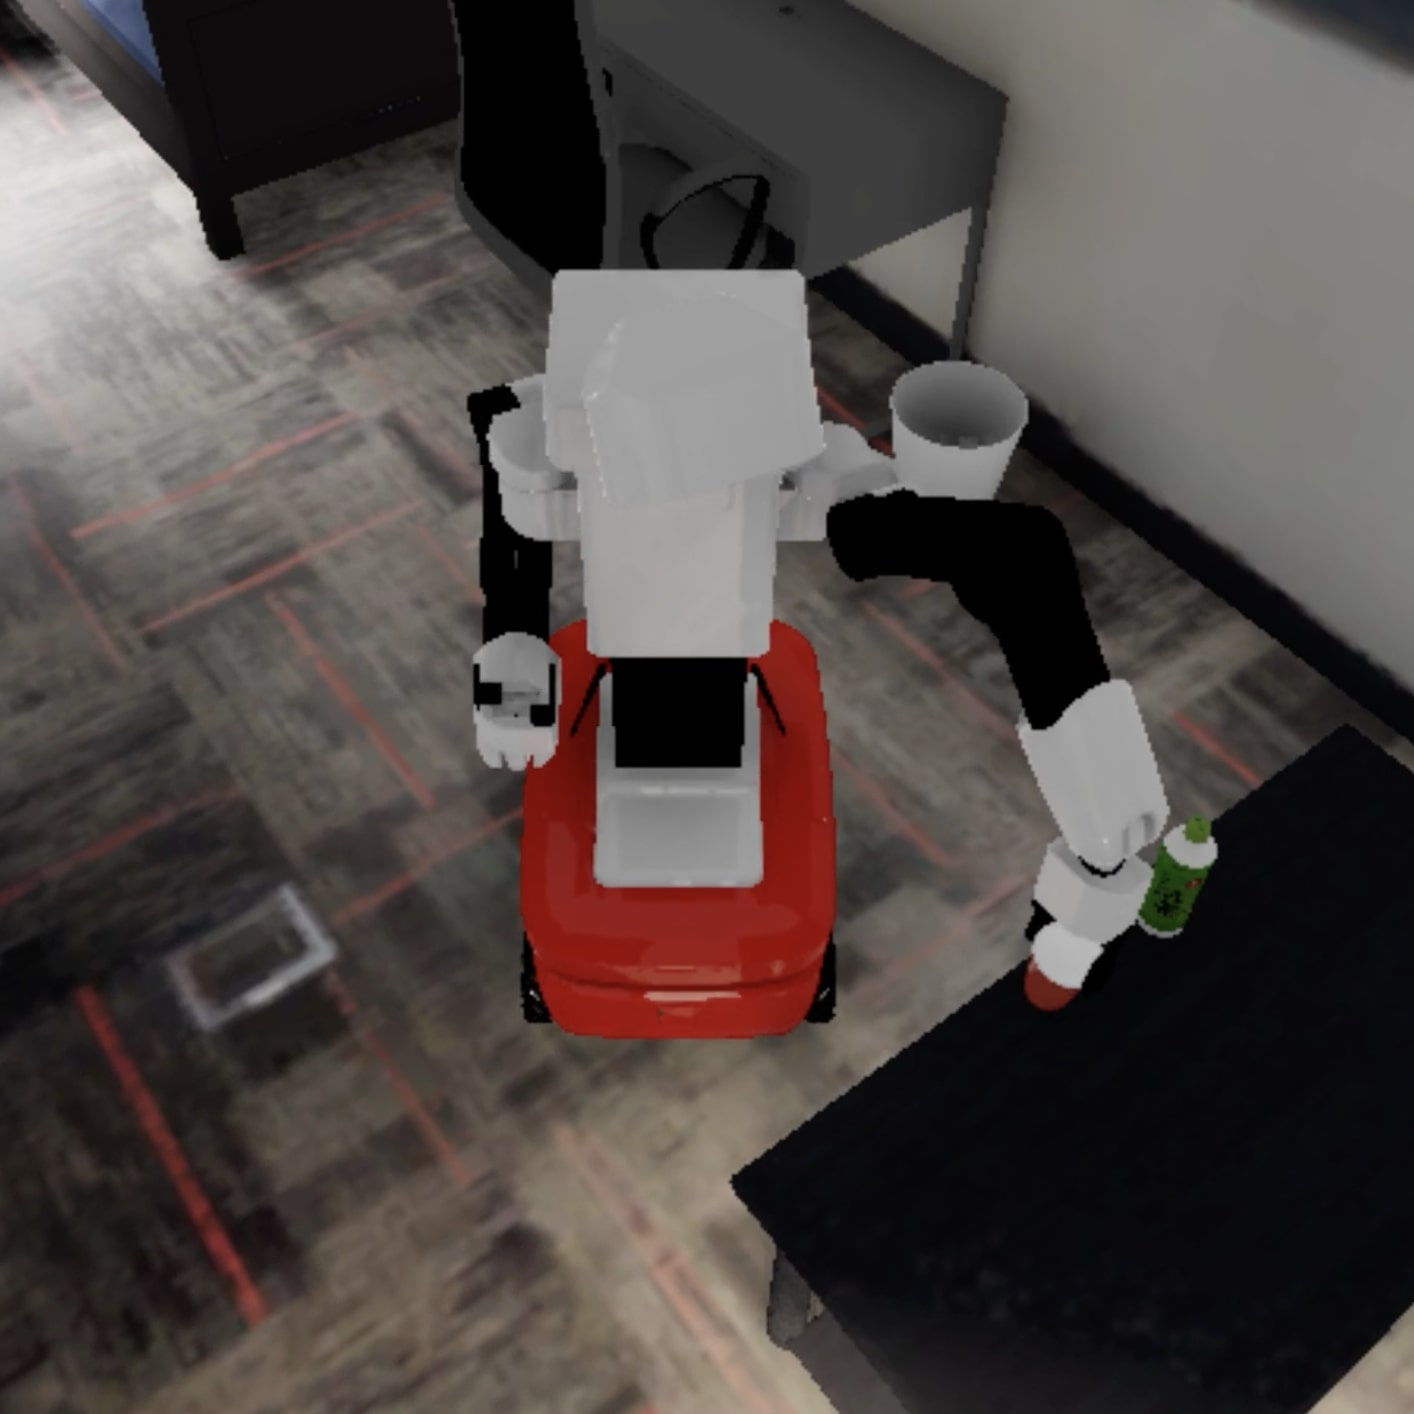
\includegraphics[trim=0 200 0 200,clip,width=0.3\linewidth]{figures/baseline_appendix/pick_2}&
%         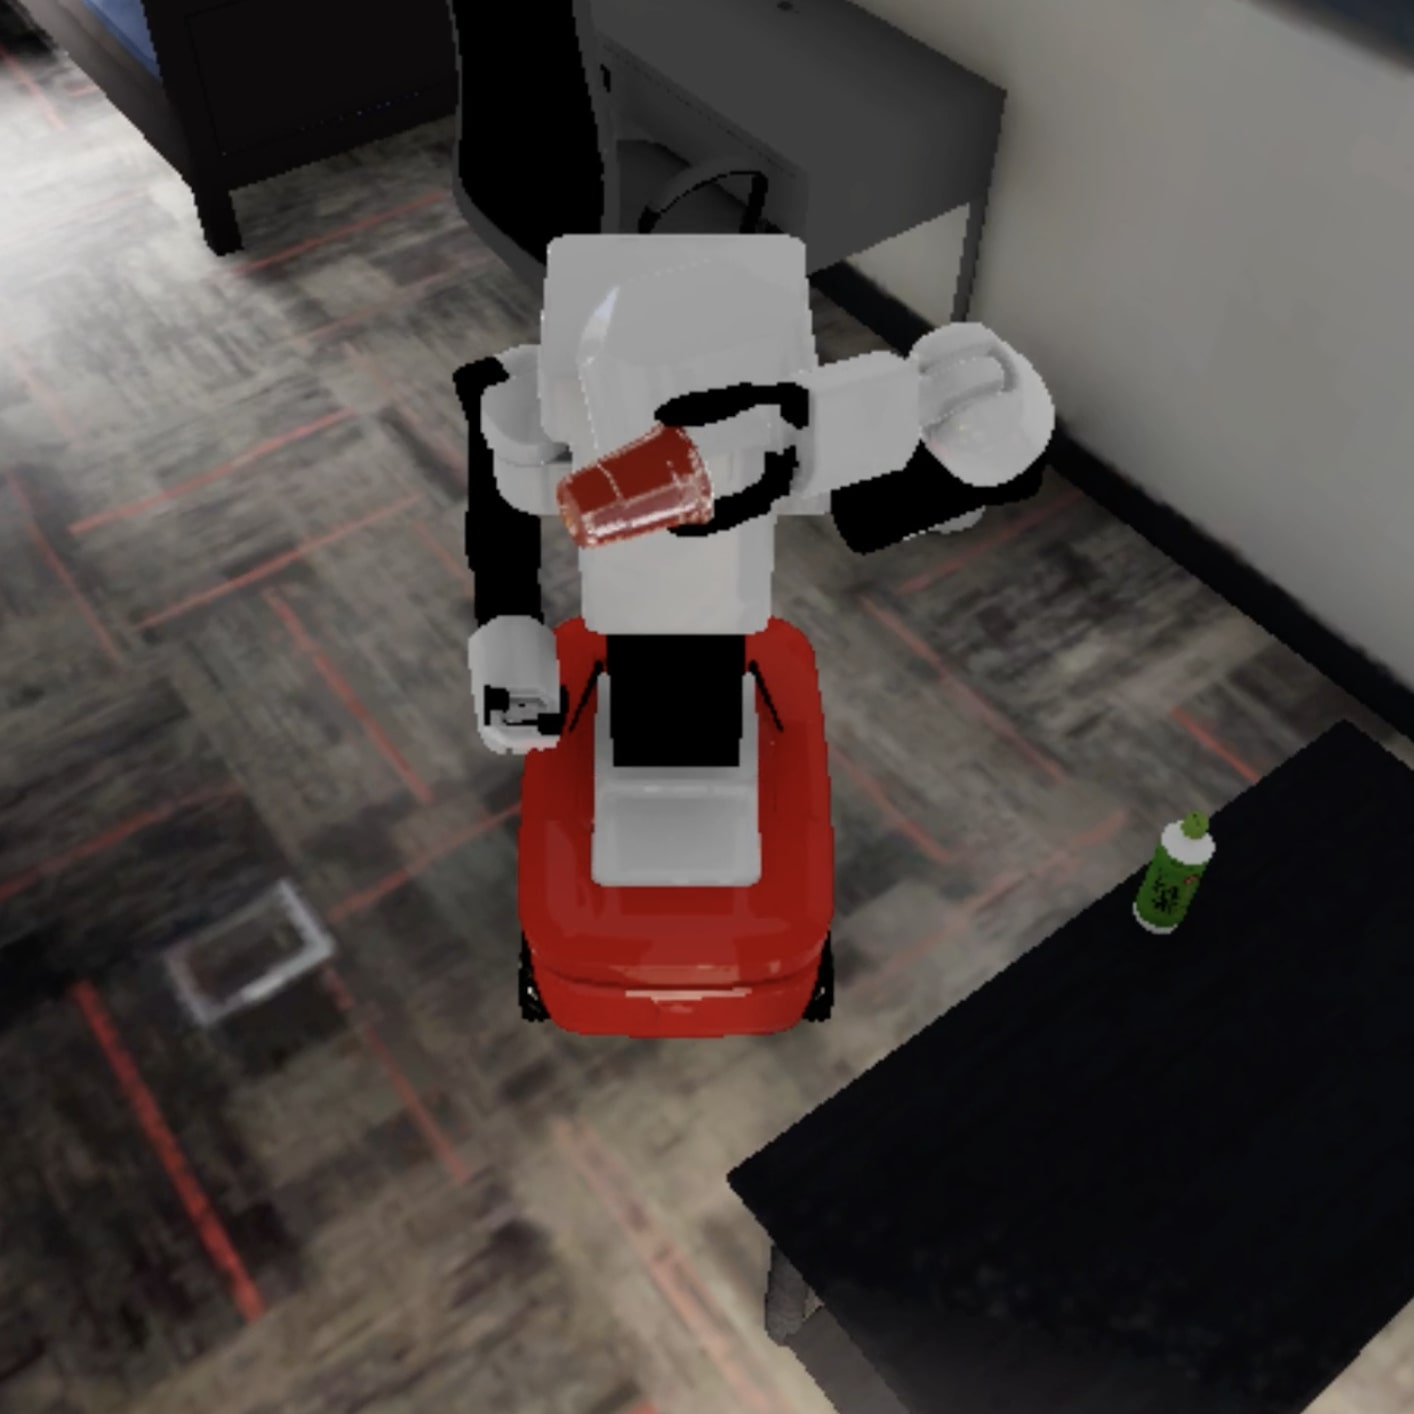
\includegraphics[trim=0 200 0 200,clip,width=0.3\linewidth]{figures/baseline_appendix/pick_3}\\
%         & b) \texttt{pick} & \\
%         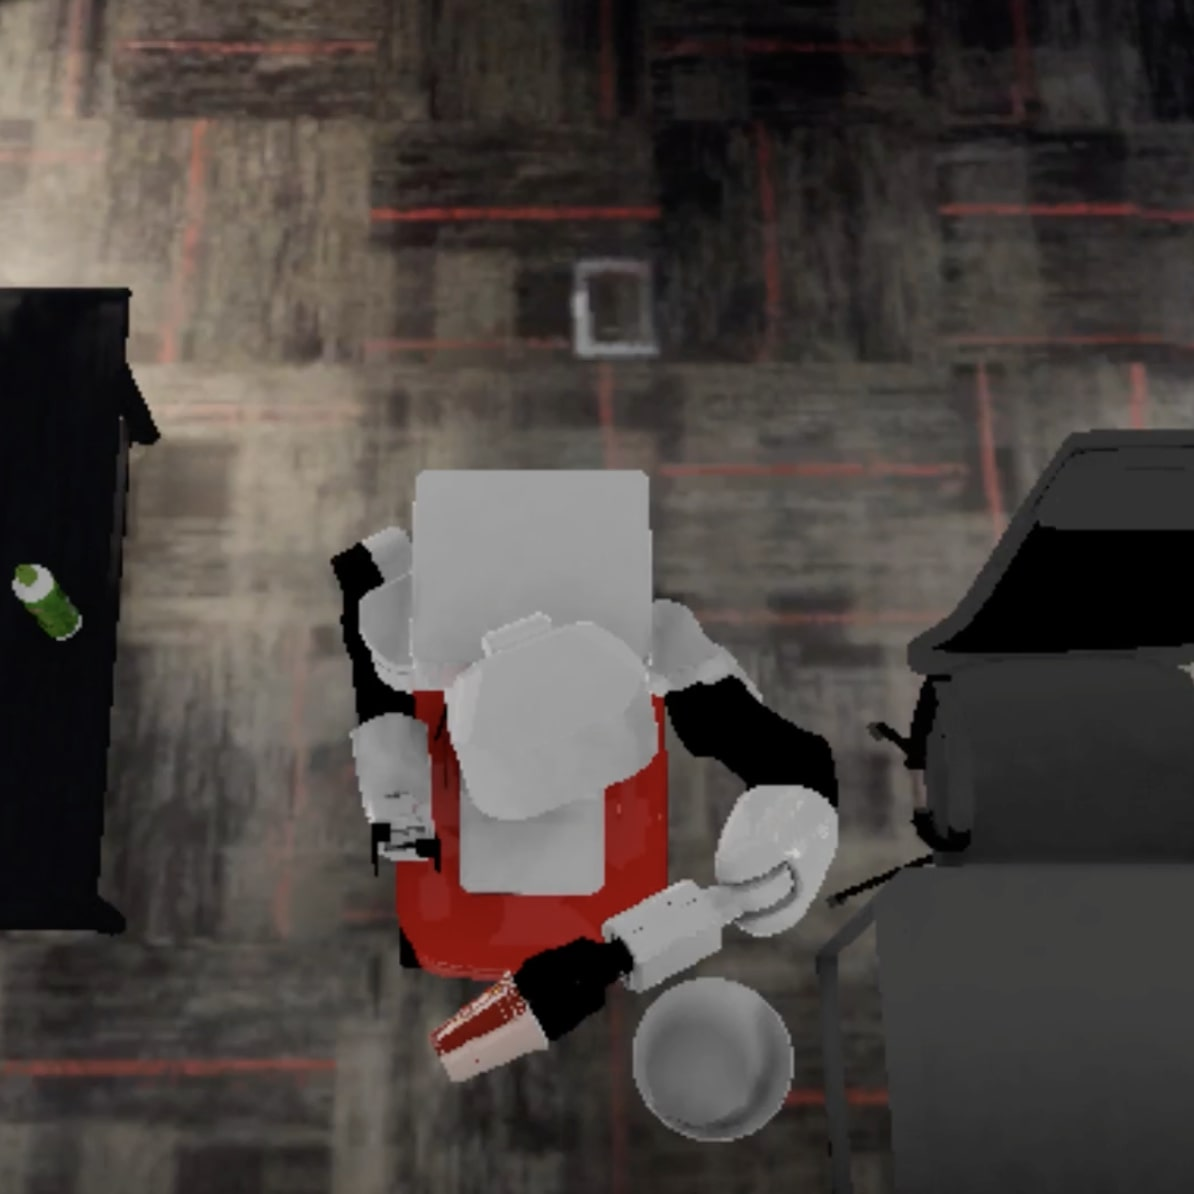
\includegraphics[trim=0 0 0 250,clip,width=0.3\linewidth]{figures/baseline_appendix/place_1}&
%         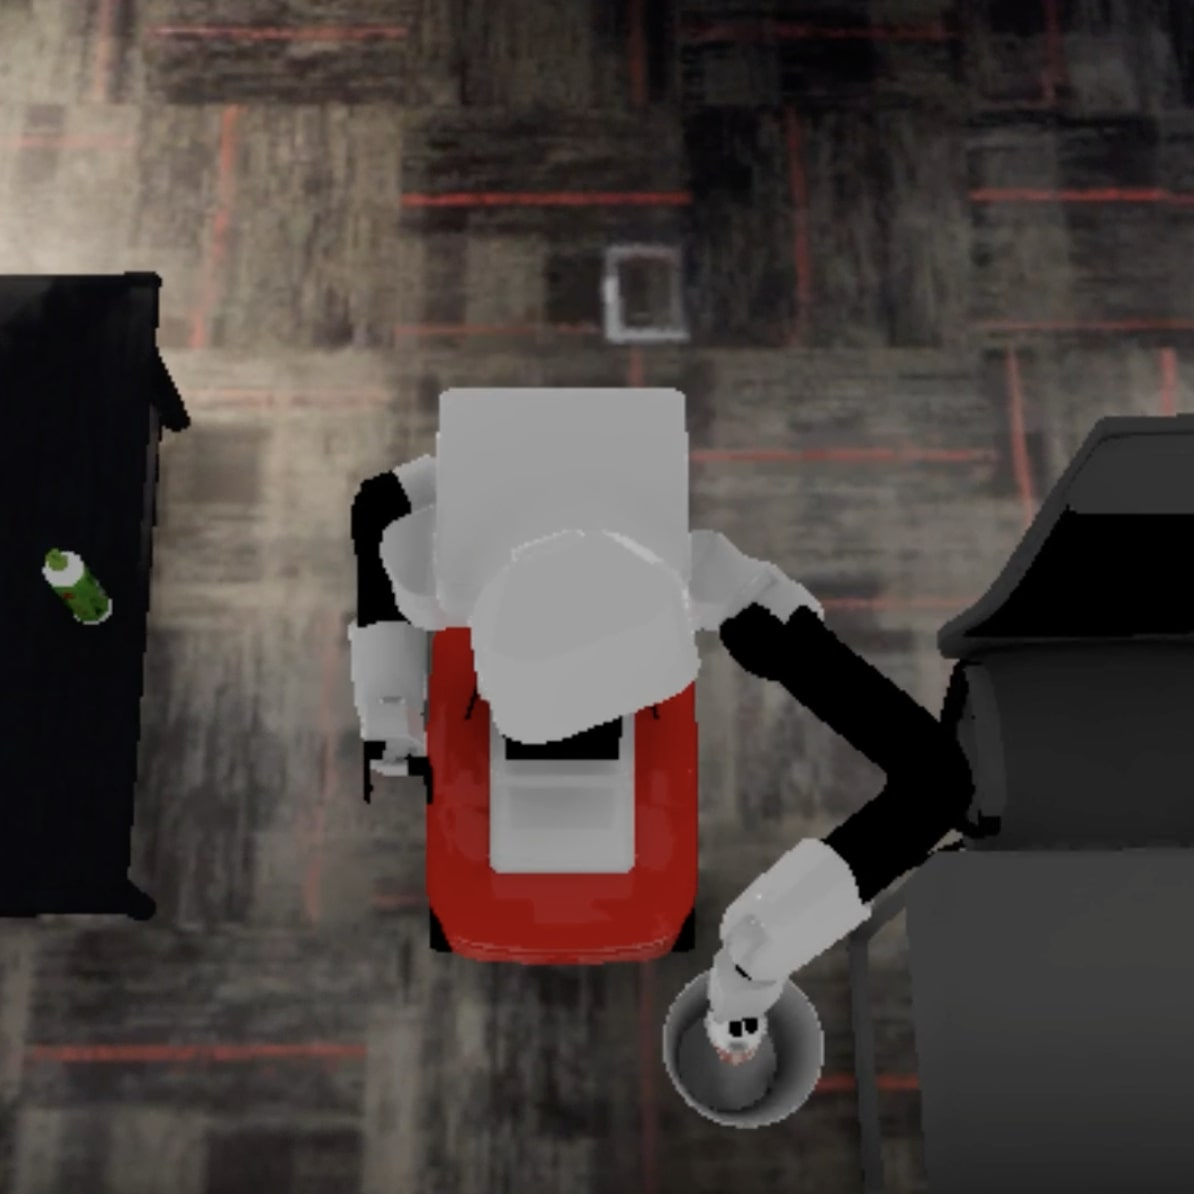
\includegraphics[trim=0 0 0 250,clip,width=0.3\linewidth]{figures/baseline_appendix/place_2}&
%         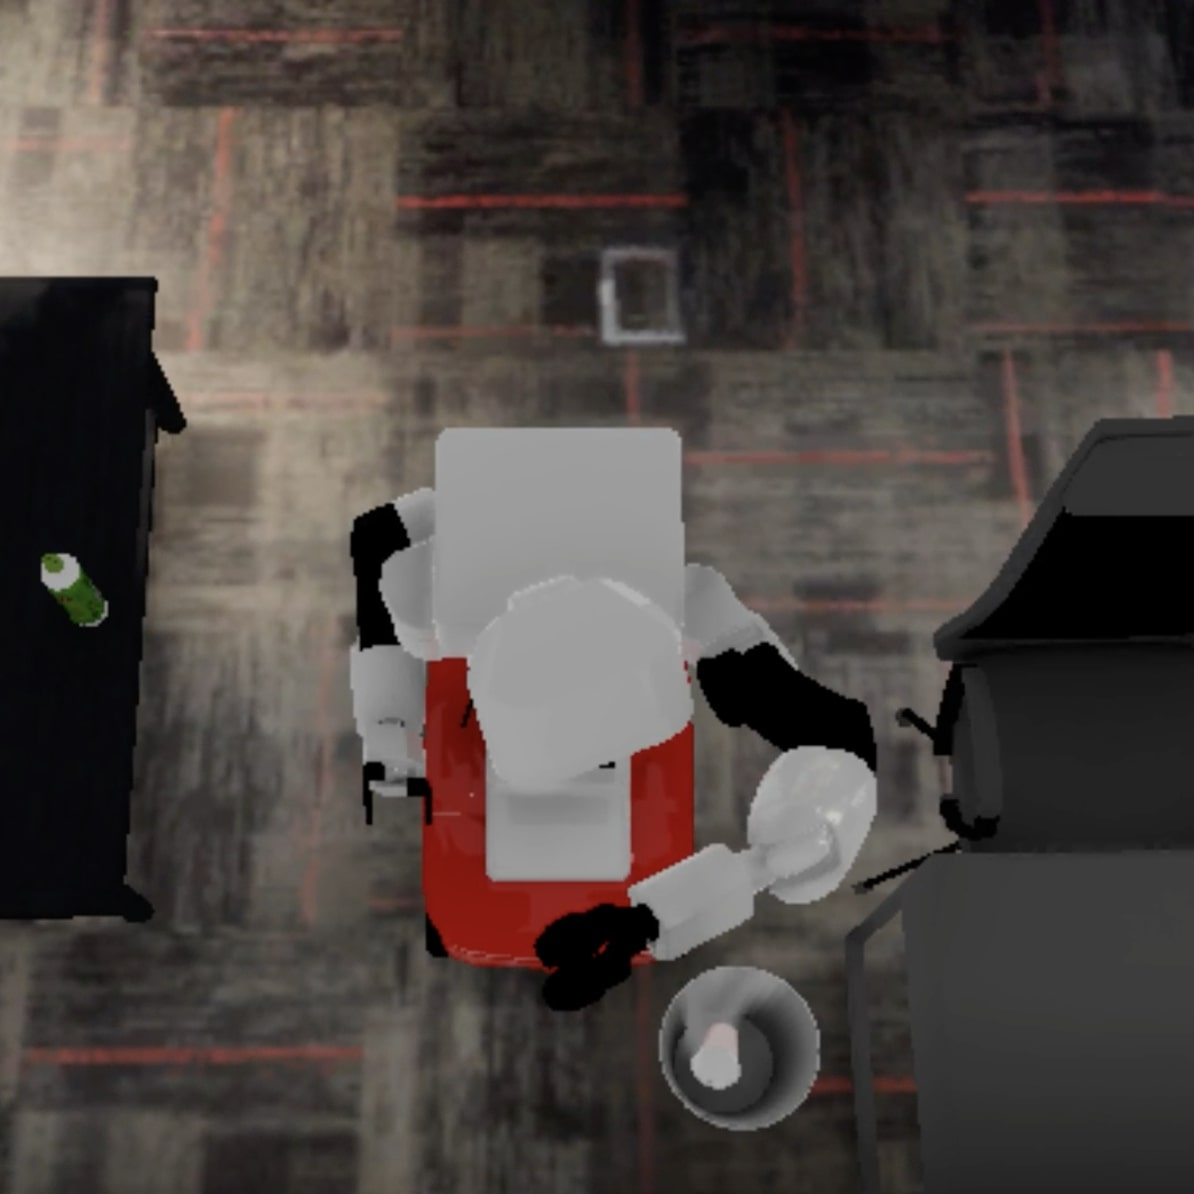
\includegraphics[trim=0 0 0 250,clip,width=0.3\linewidth]{figures/baseline_appendix/place_3}\\
%         & c) \texttt{place} & \\
%         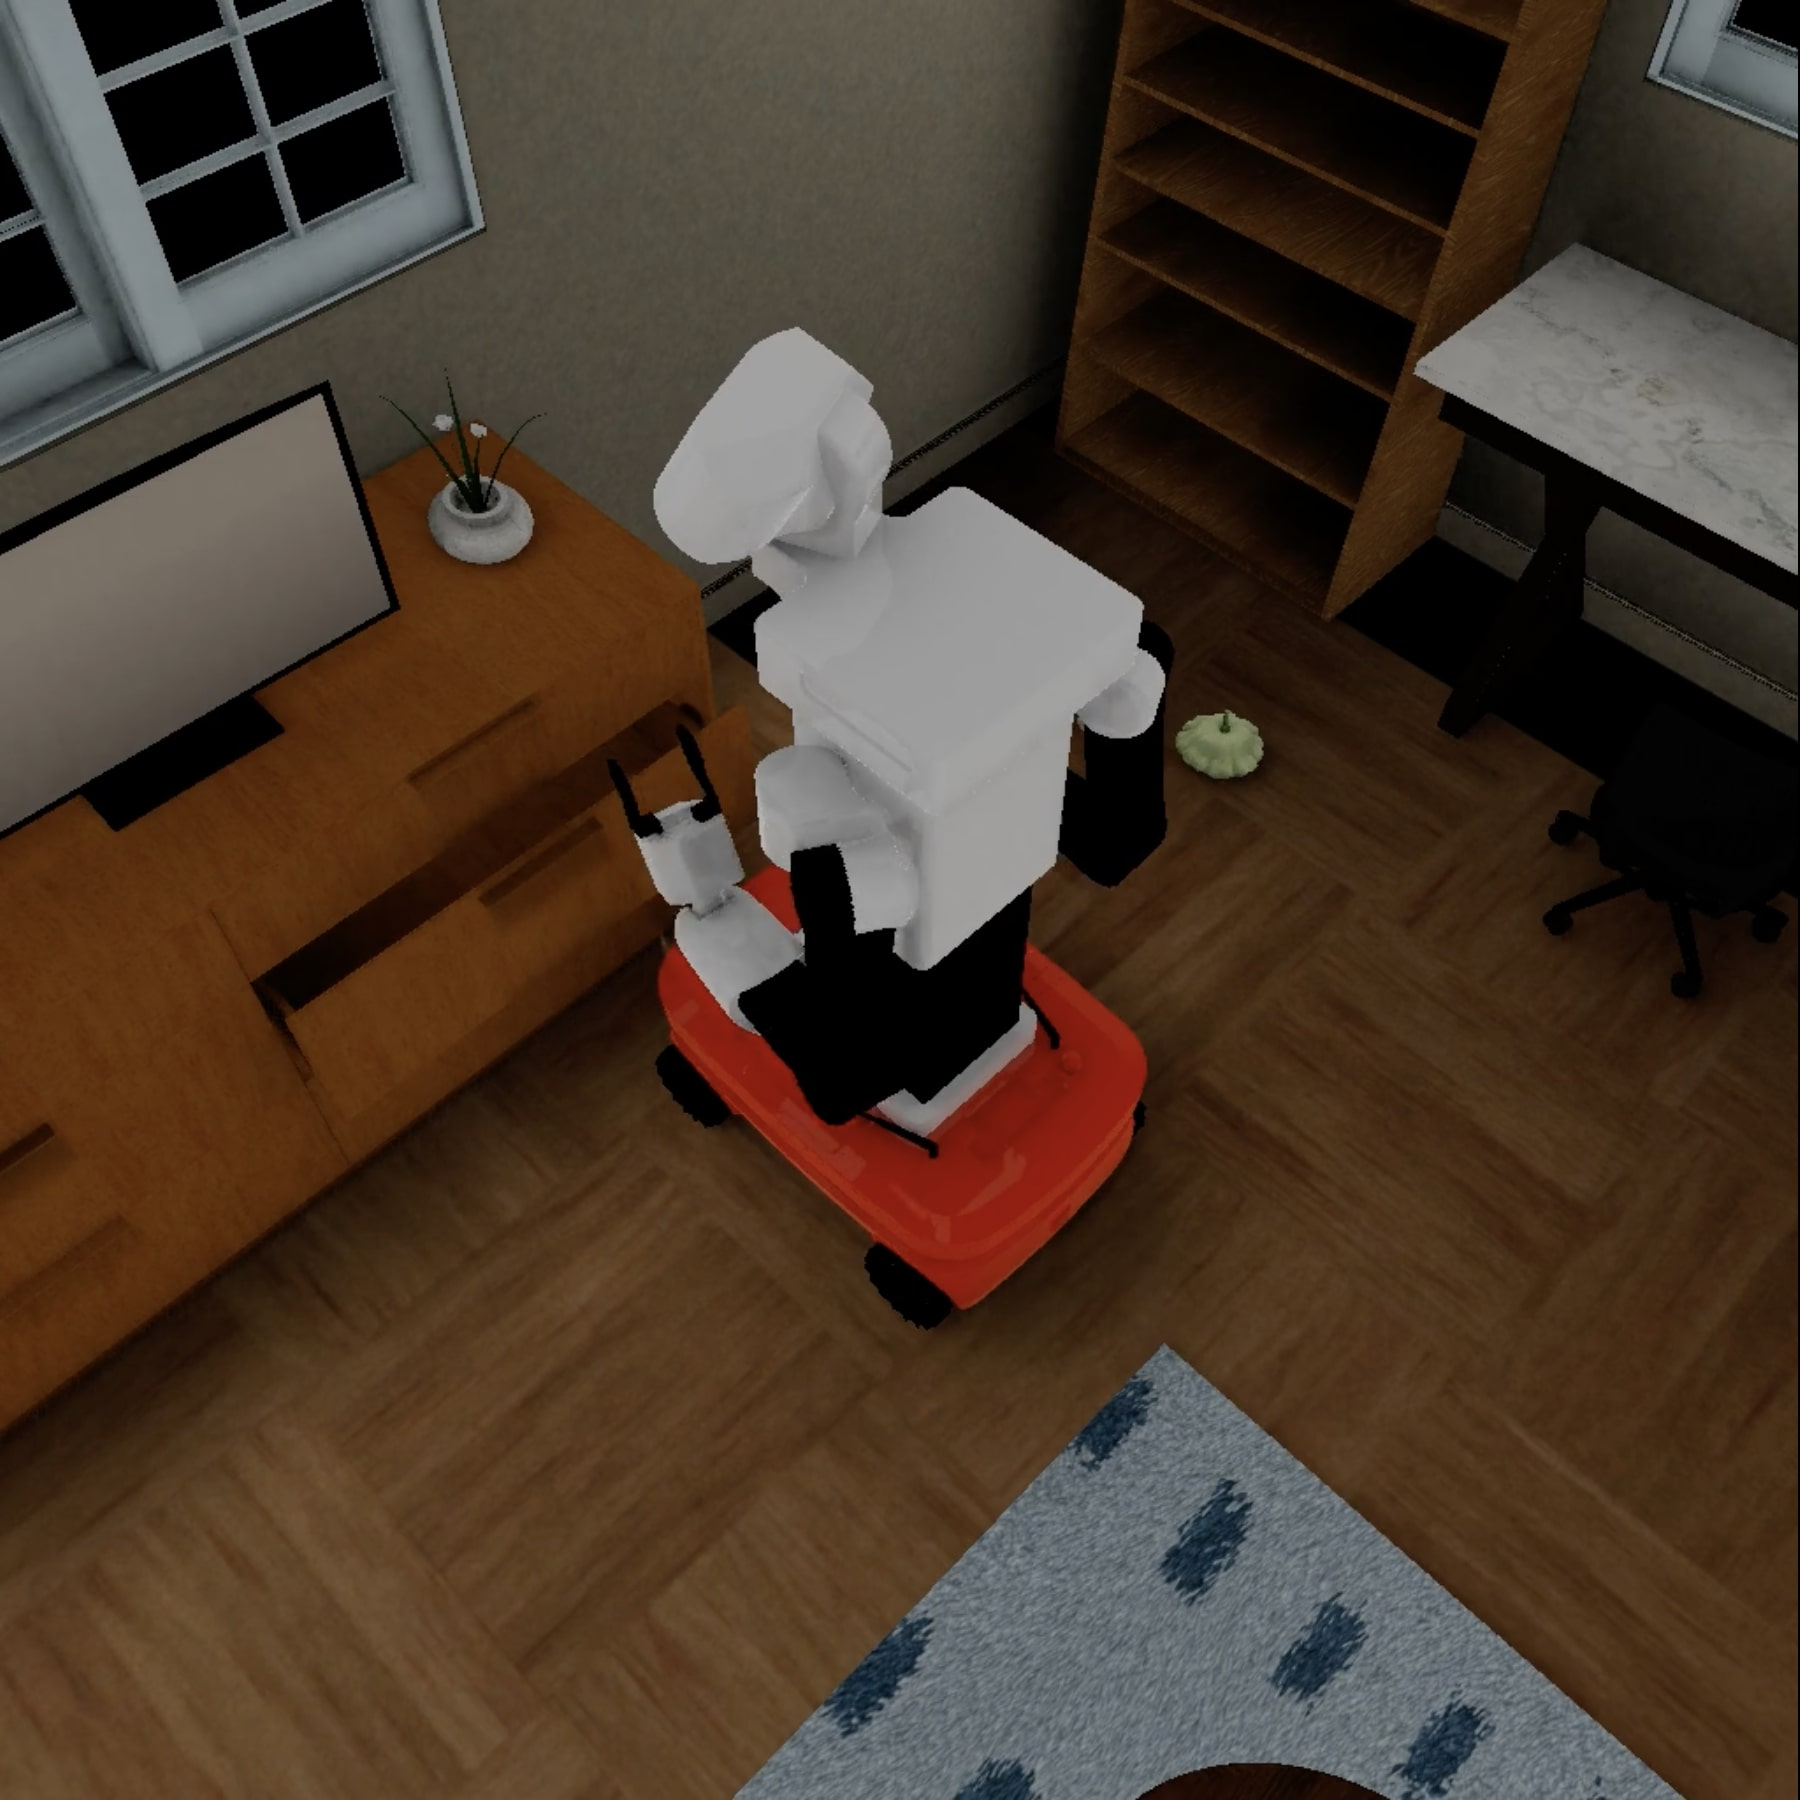
\includegraphics[trim=0 220 0 20,clip,width=0.3\linewidth]{figures/baseline_appendix/pull_1}&
%         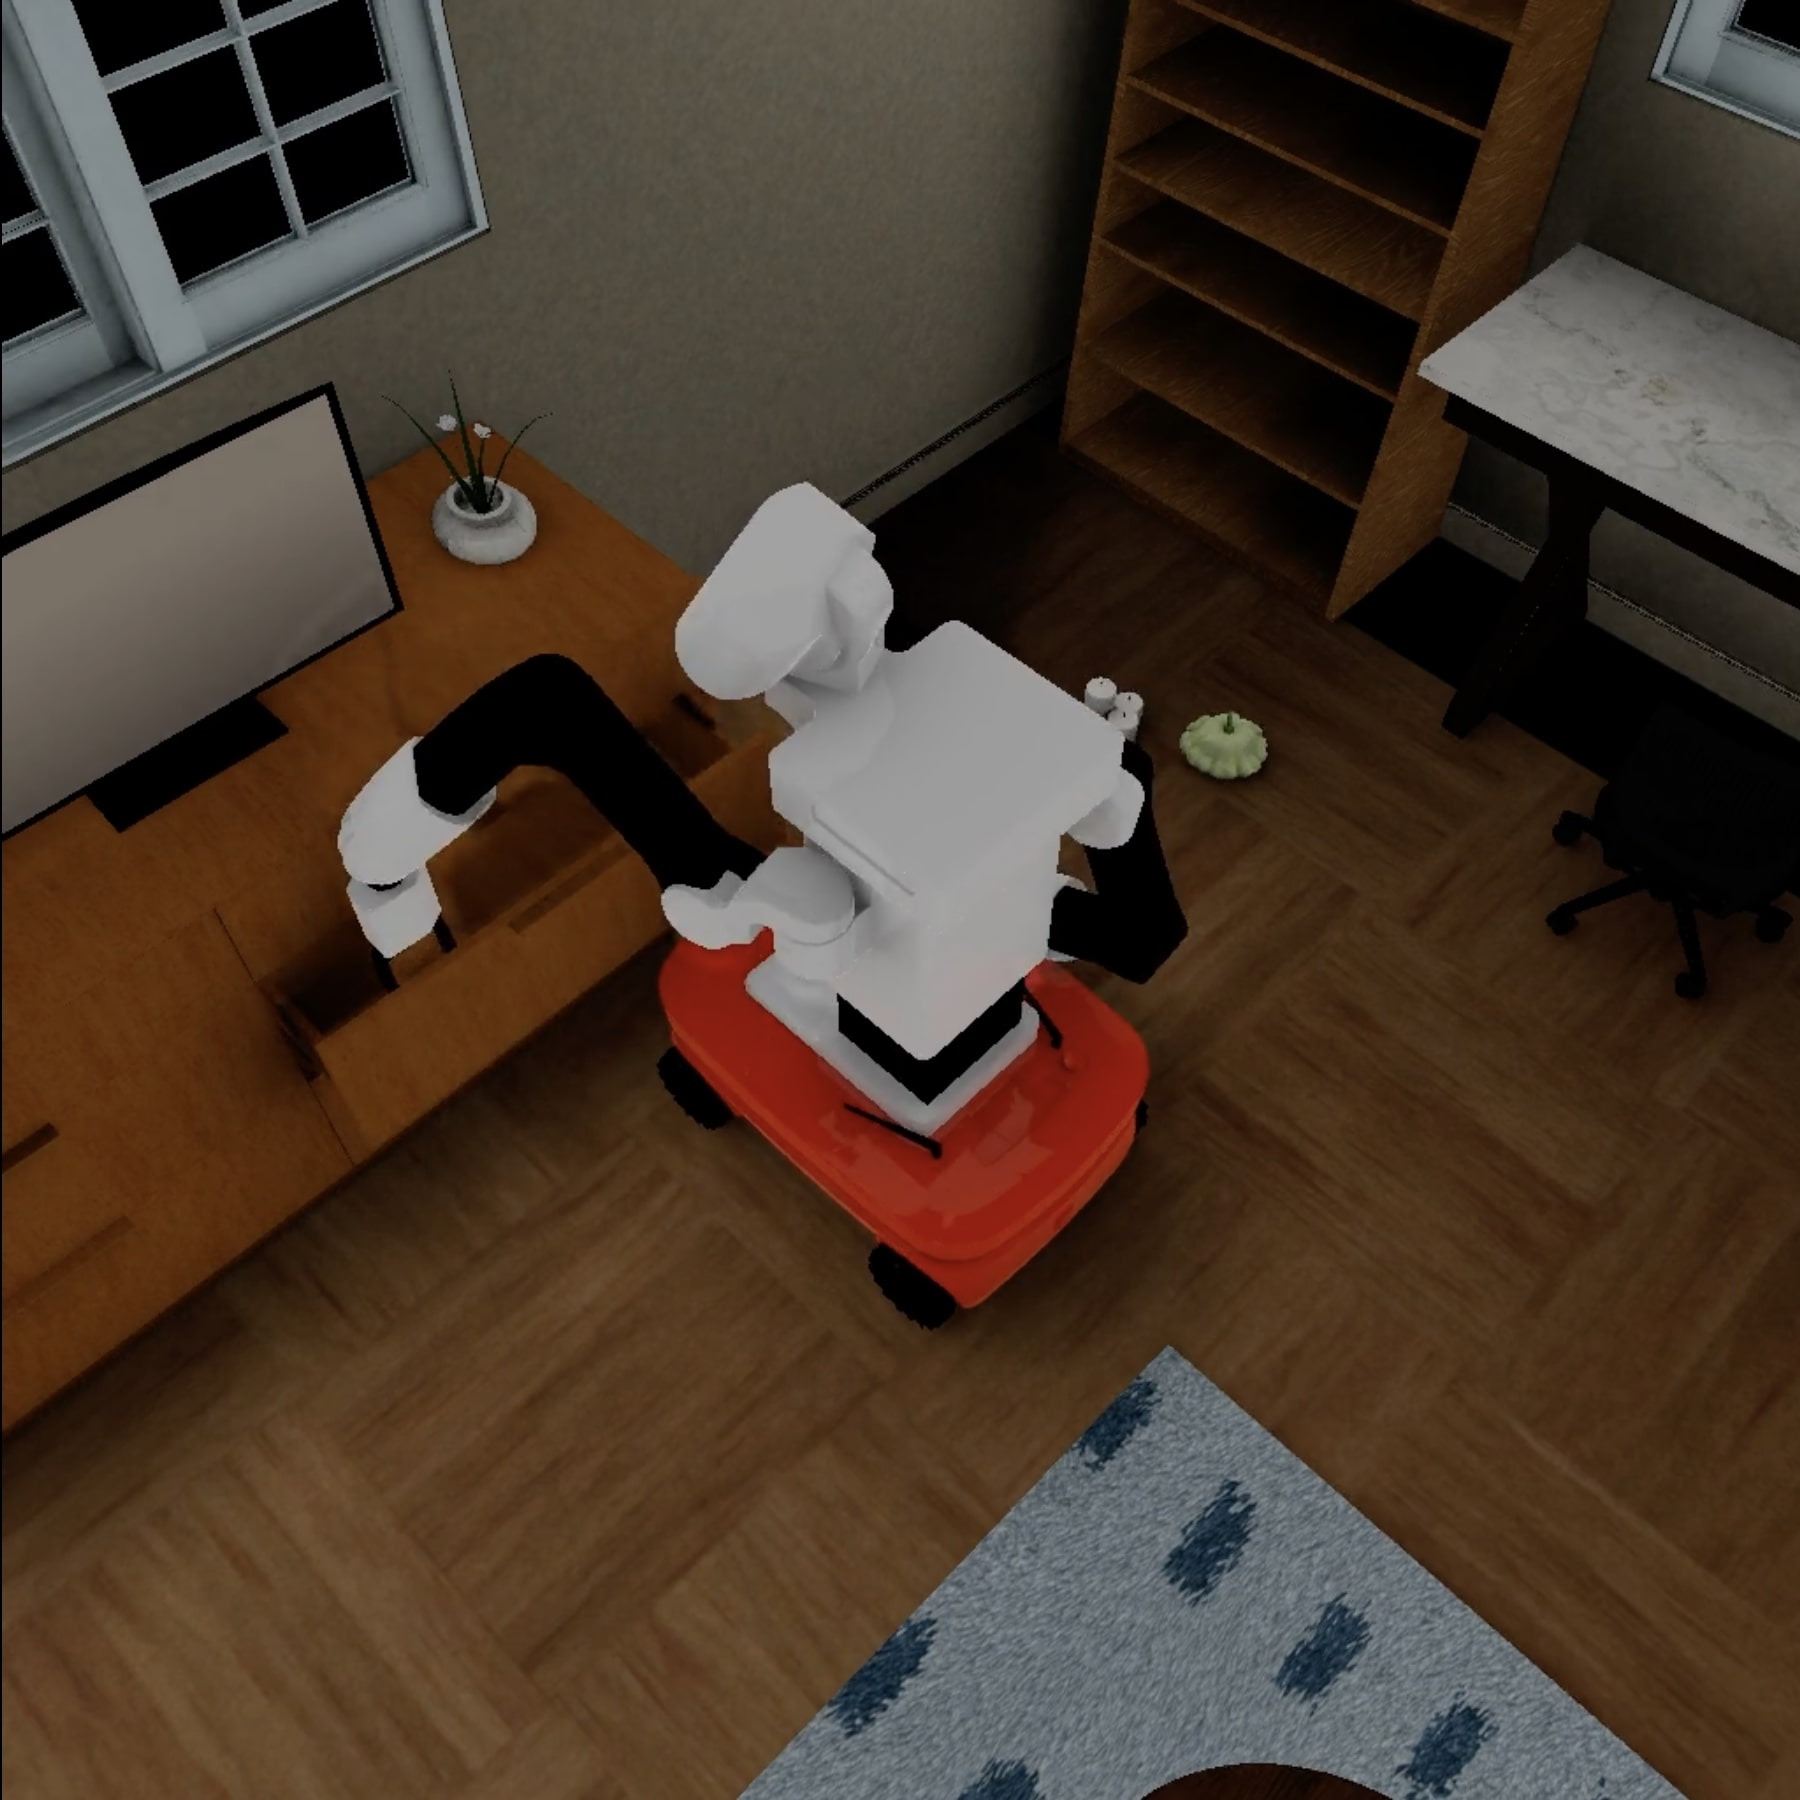
\includegraphics[trim=0 220 0 20,clip,width=0.3\linewidth]{figures/baseline_appendix/pull_2}&
%         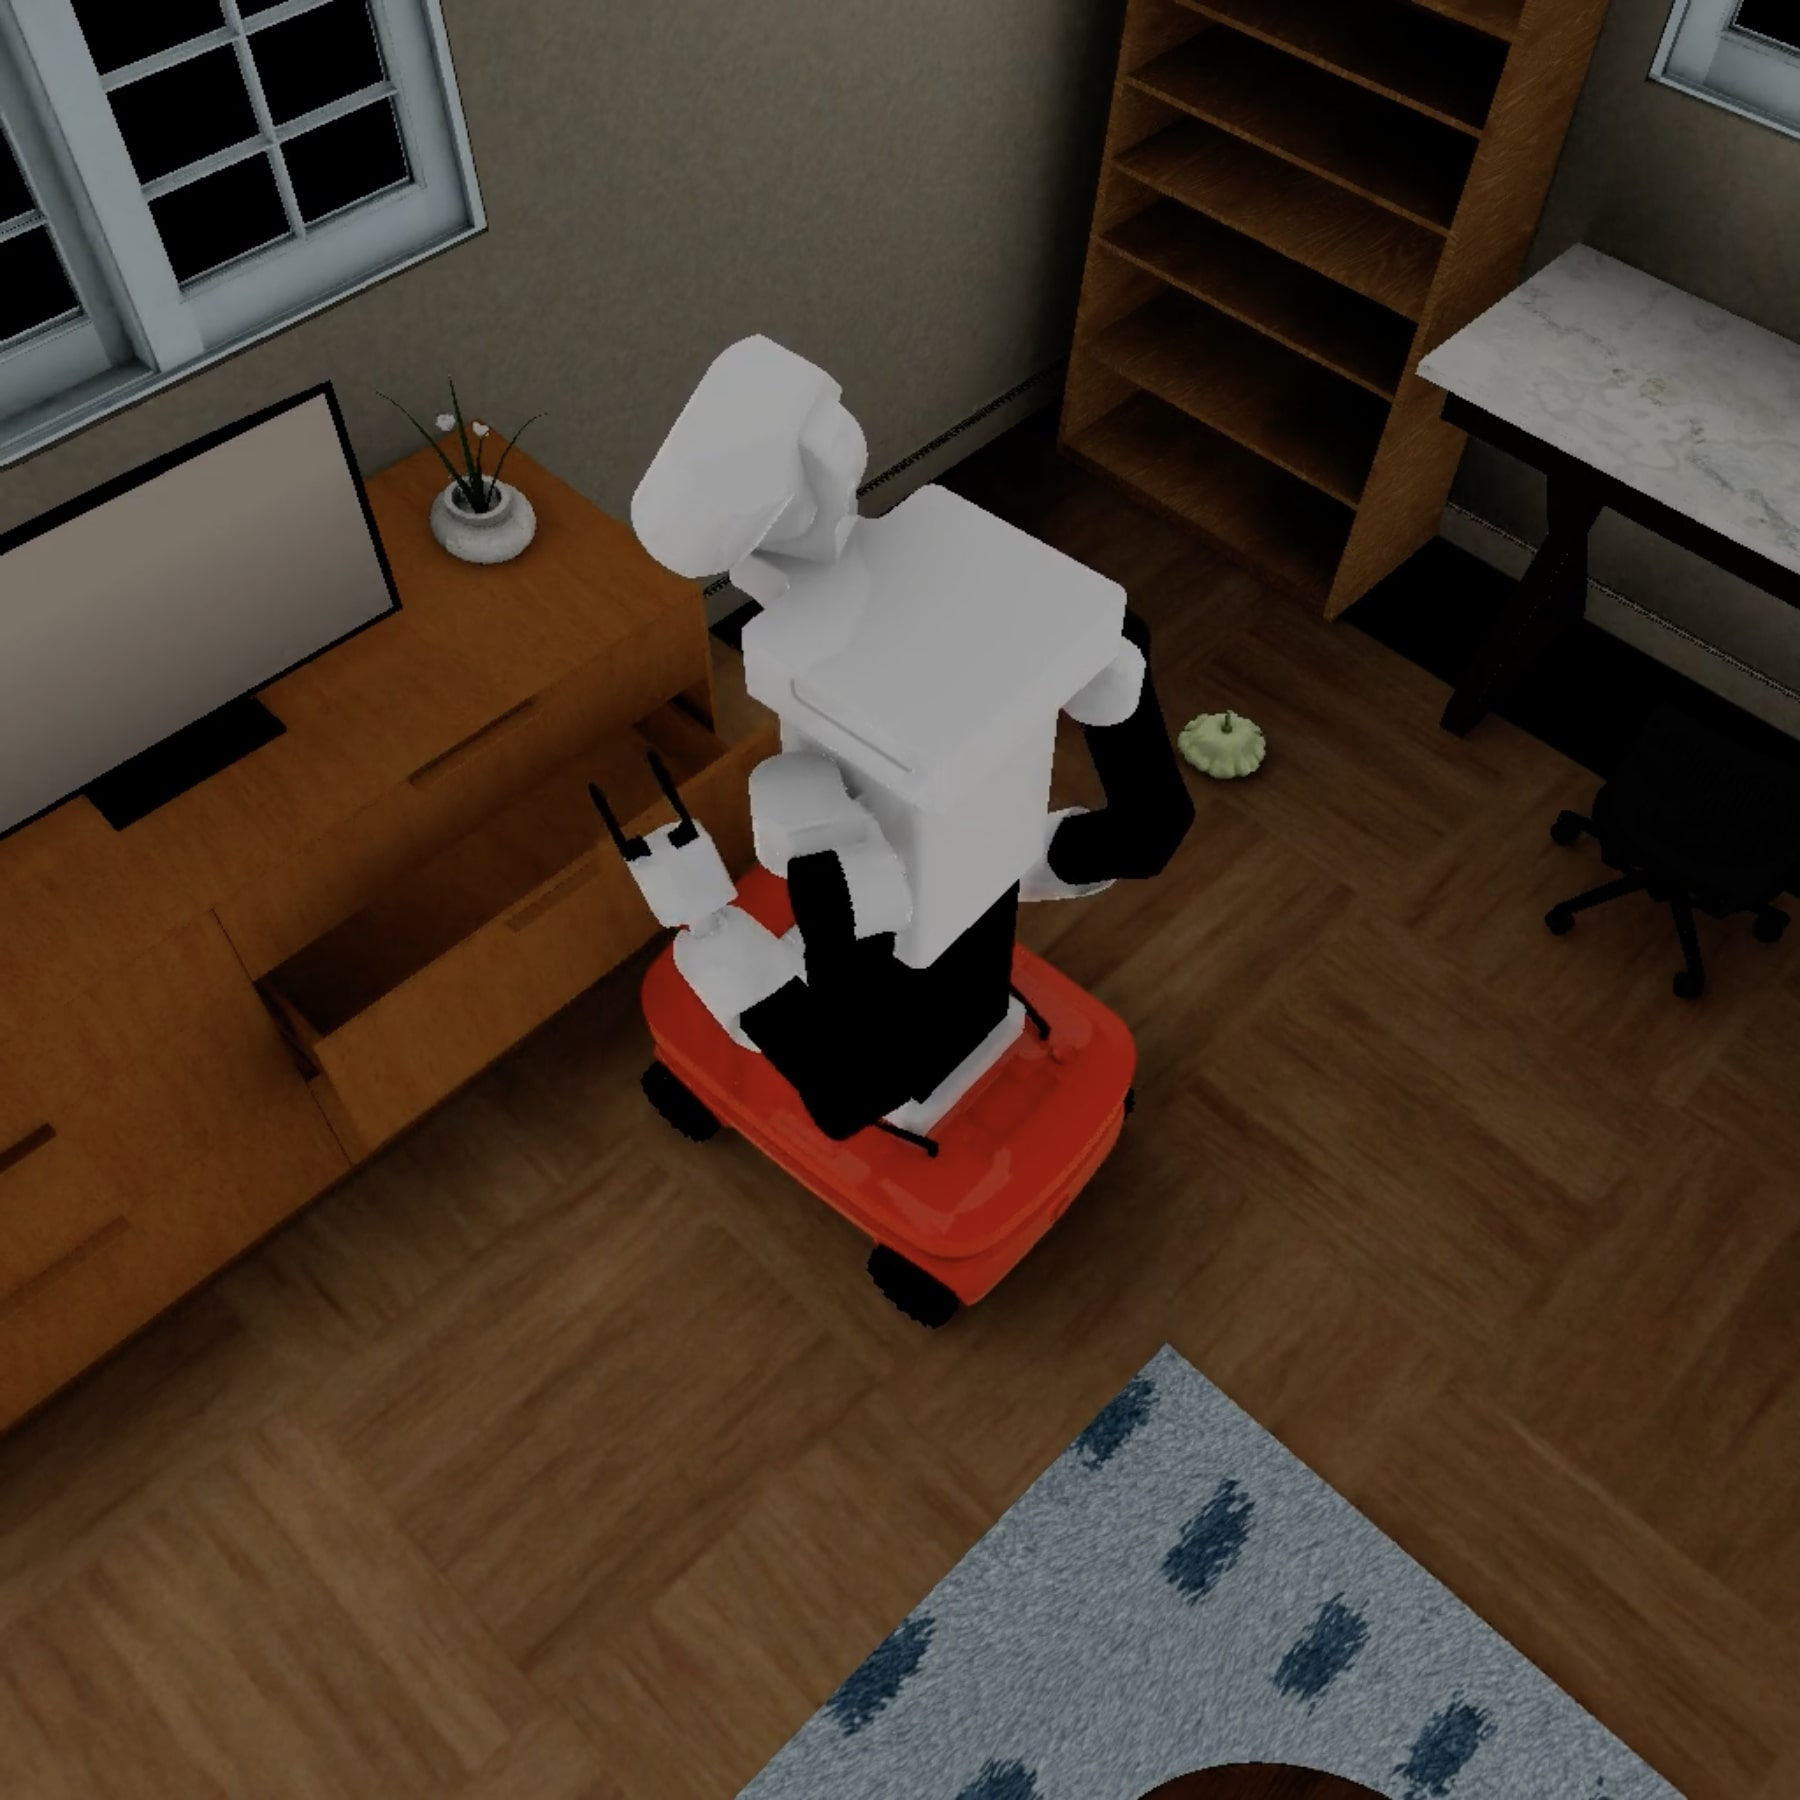
\includegraphics[trim=0 220 0 20,clip,width=0.3\linewidth]{figures/baseline_appendix/pull_3}\\
%         & d) \texttt{push} & \\
%         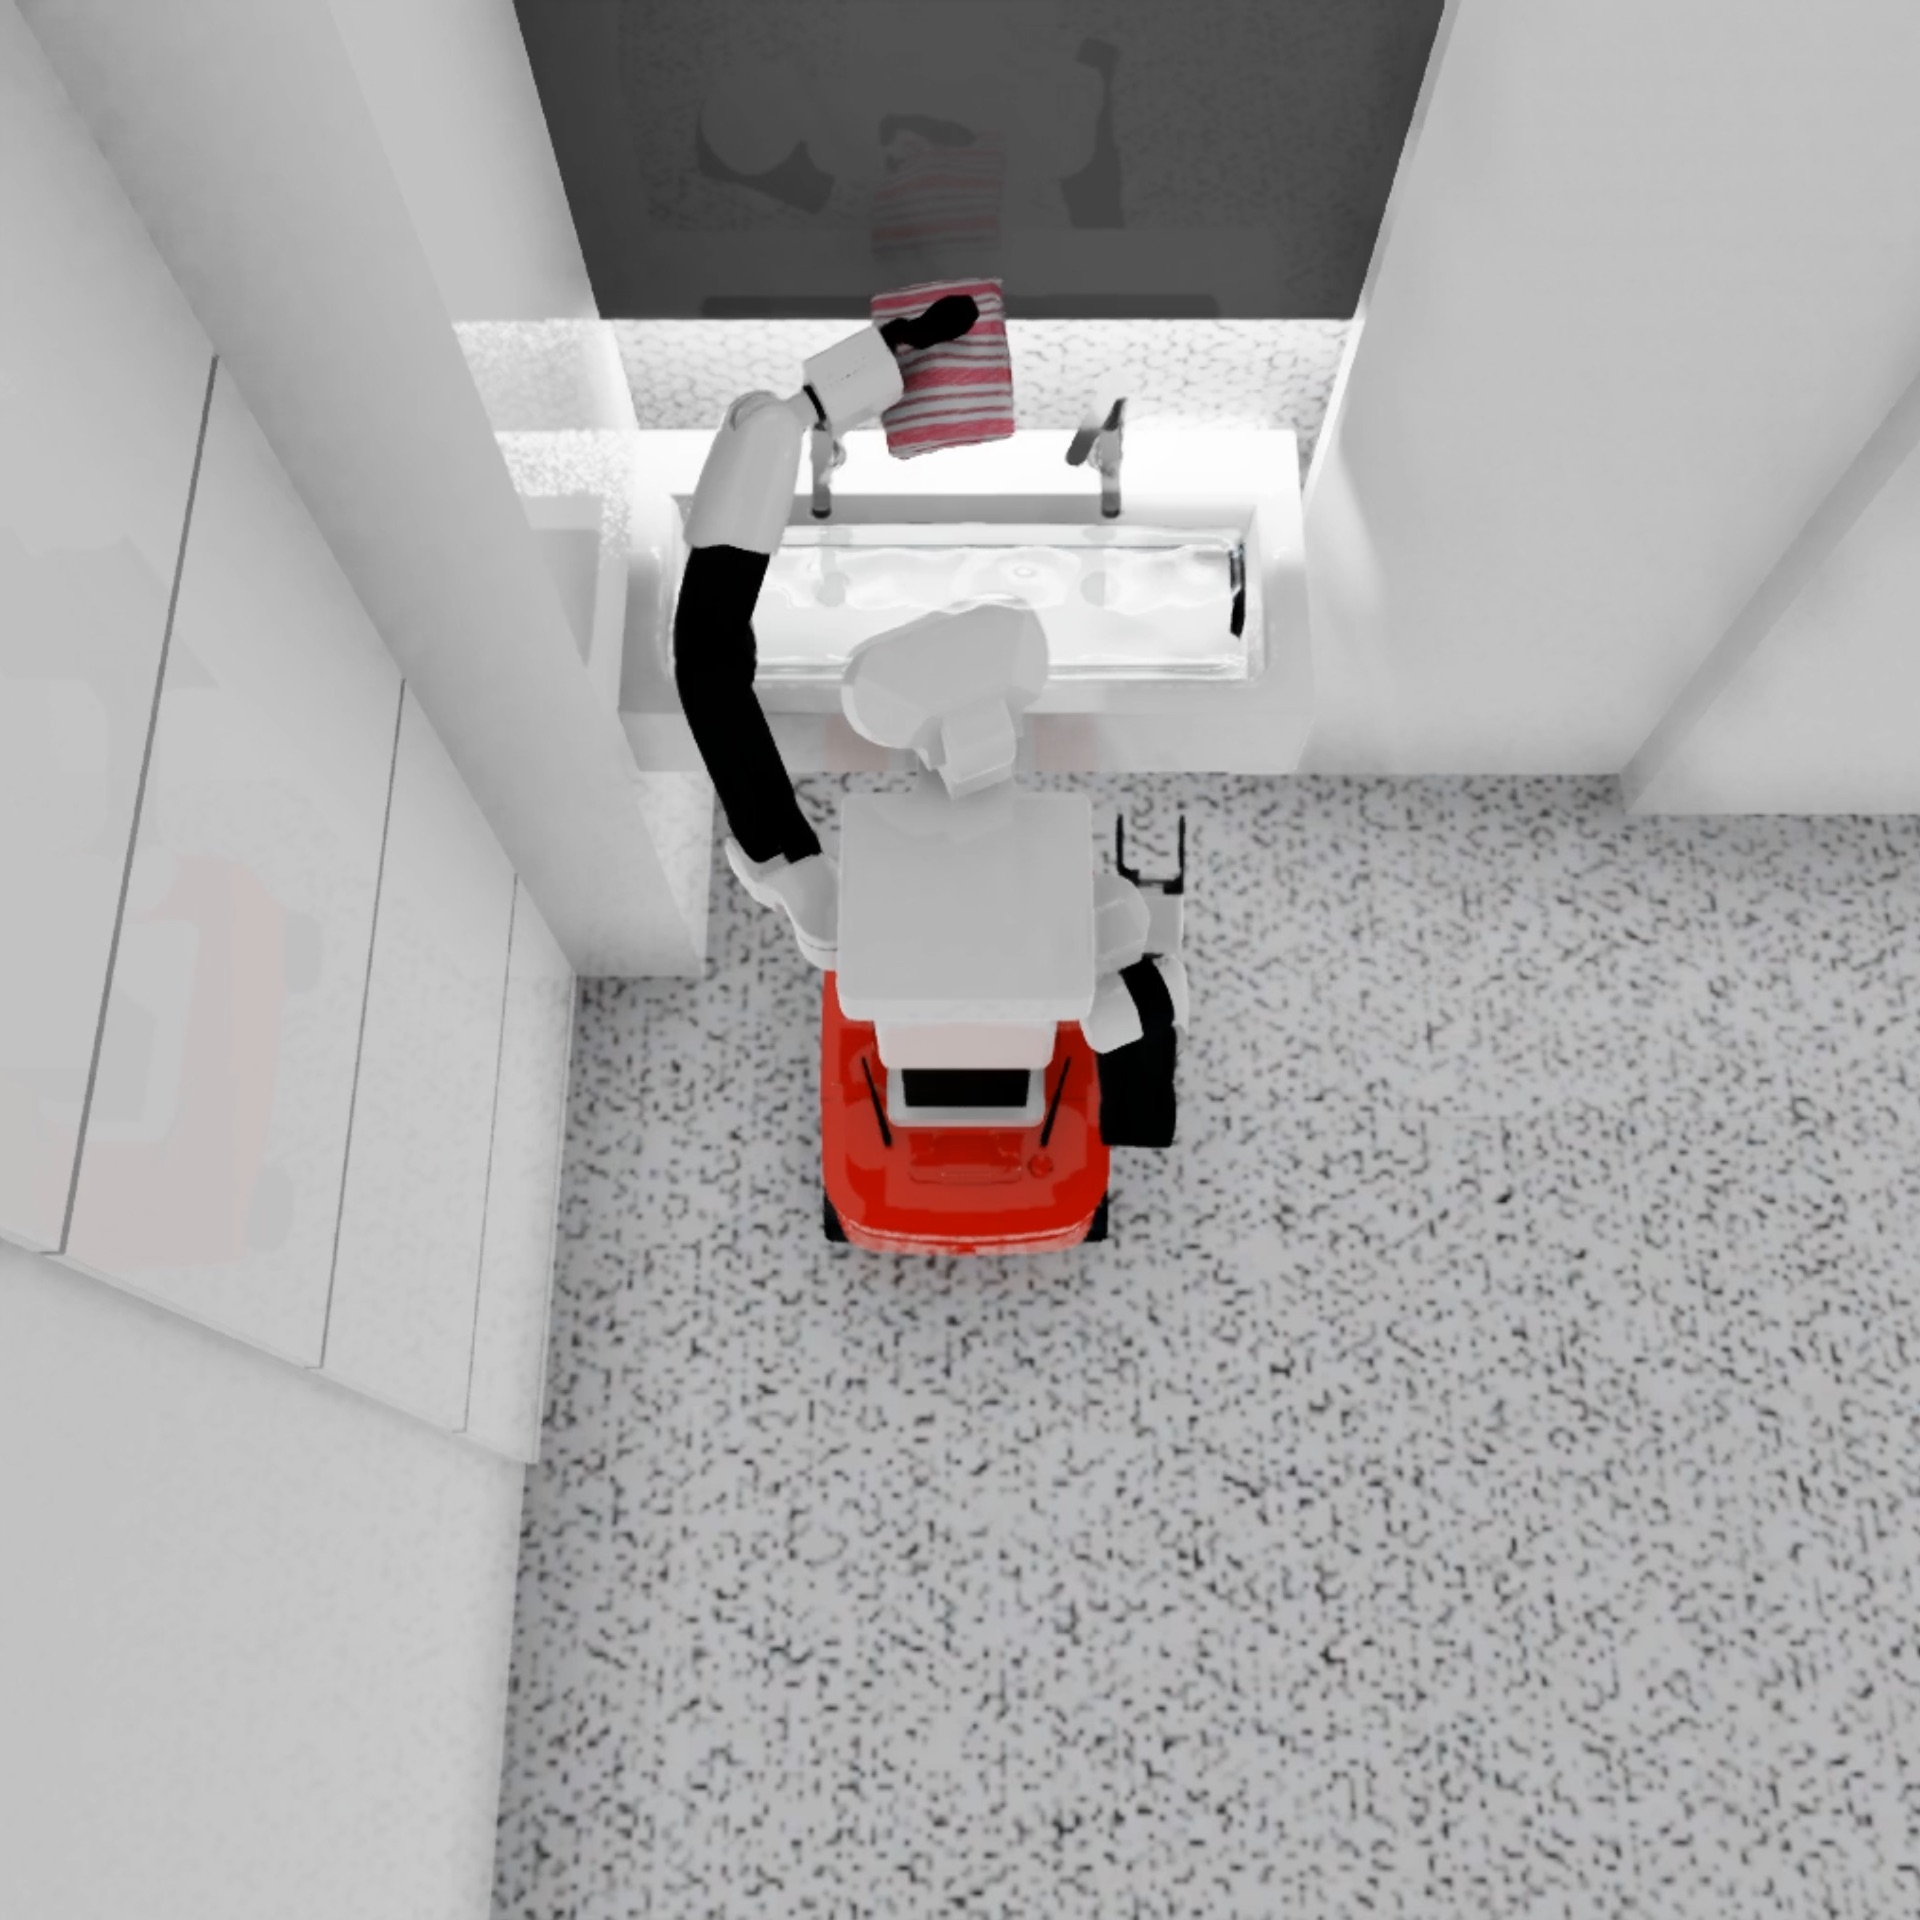
\includegraphics[trim=0 200 0 100,clip,width=0.3\linewidth]{figures/baseline_appendix/dip_1}&
%         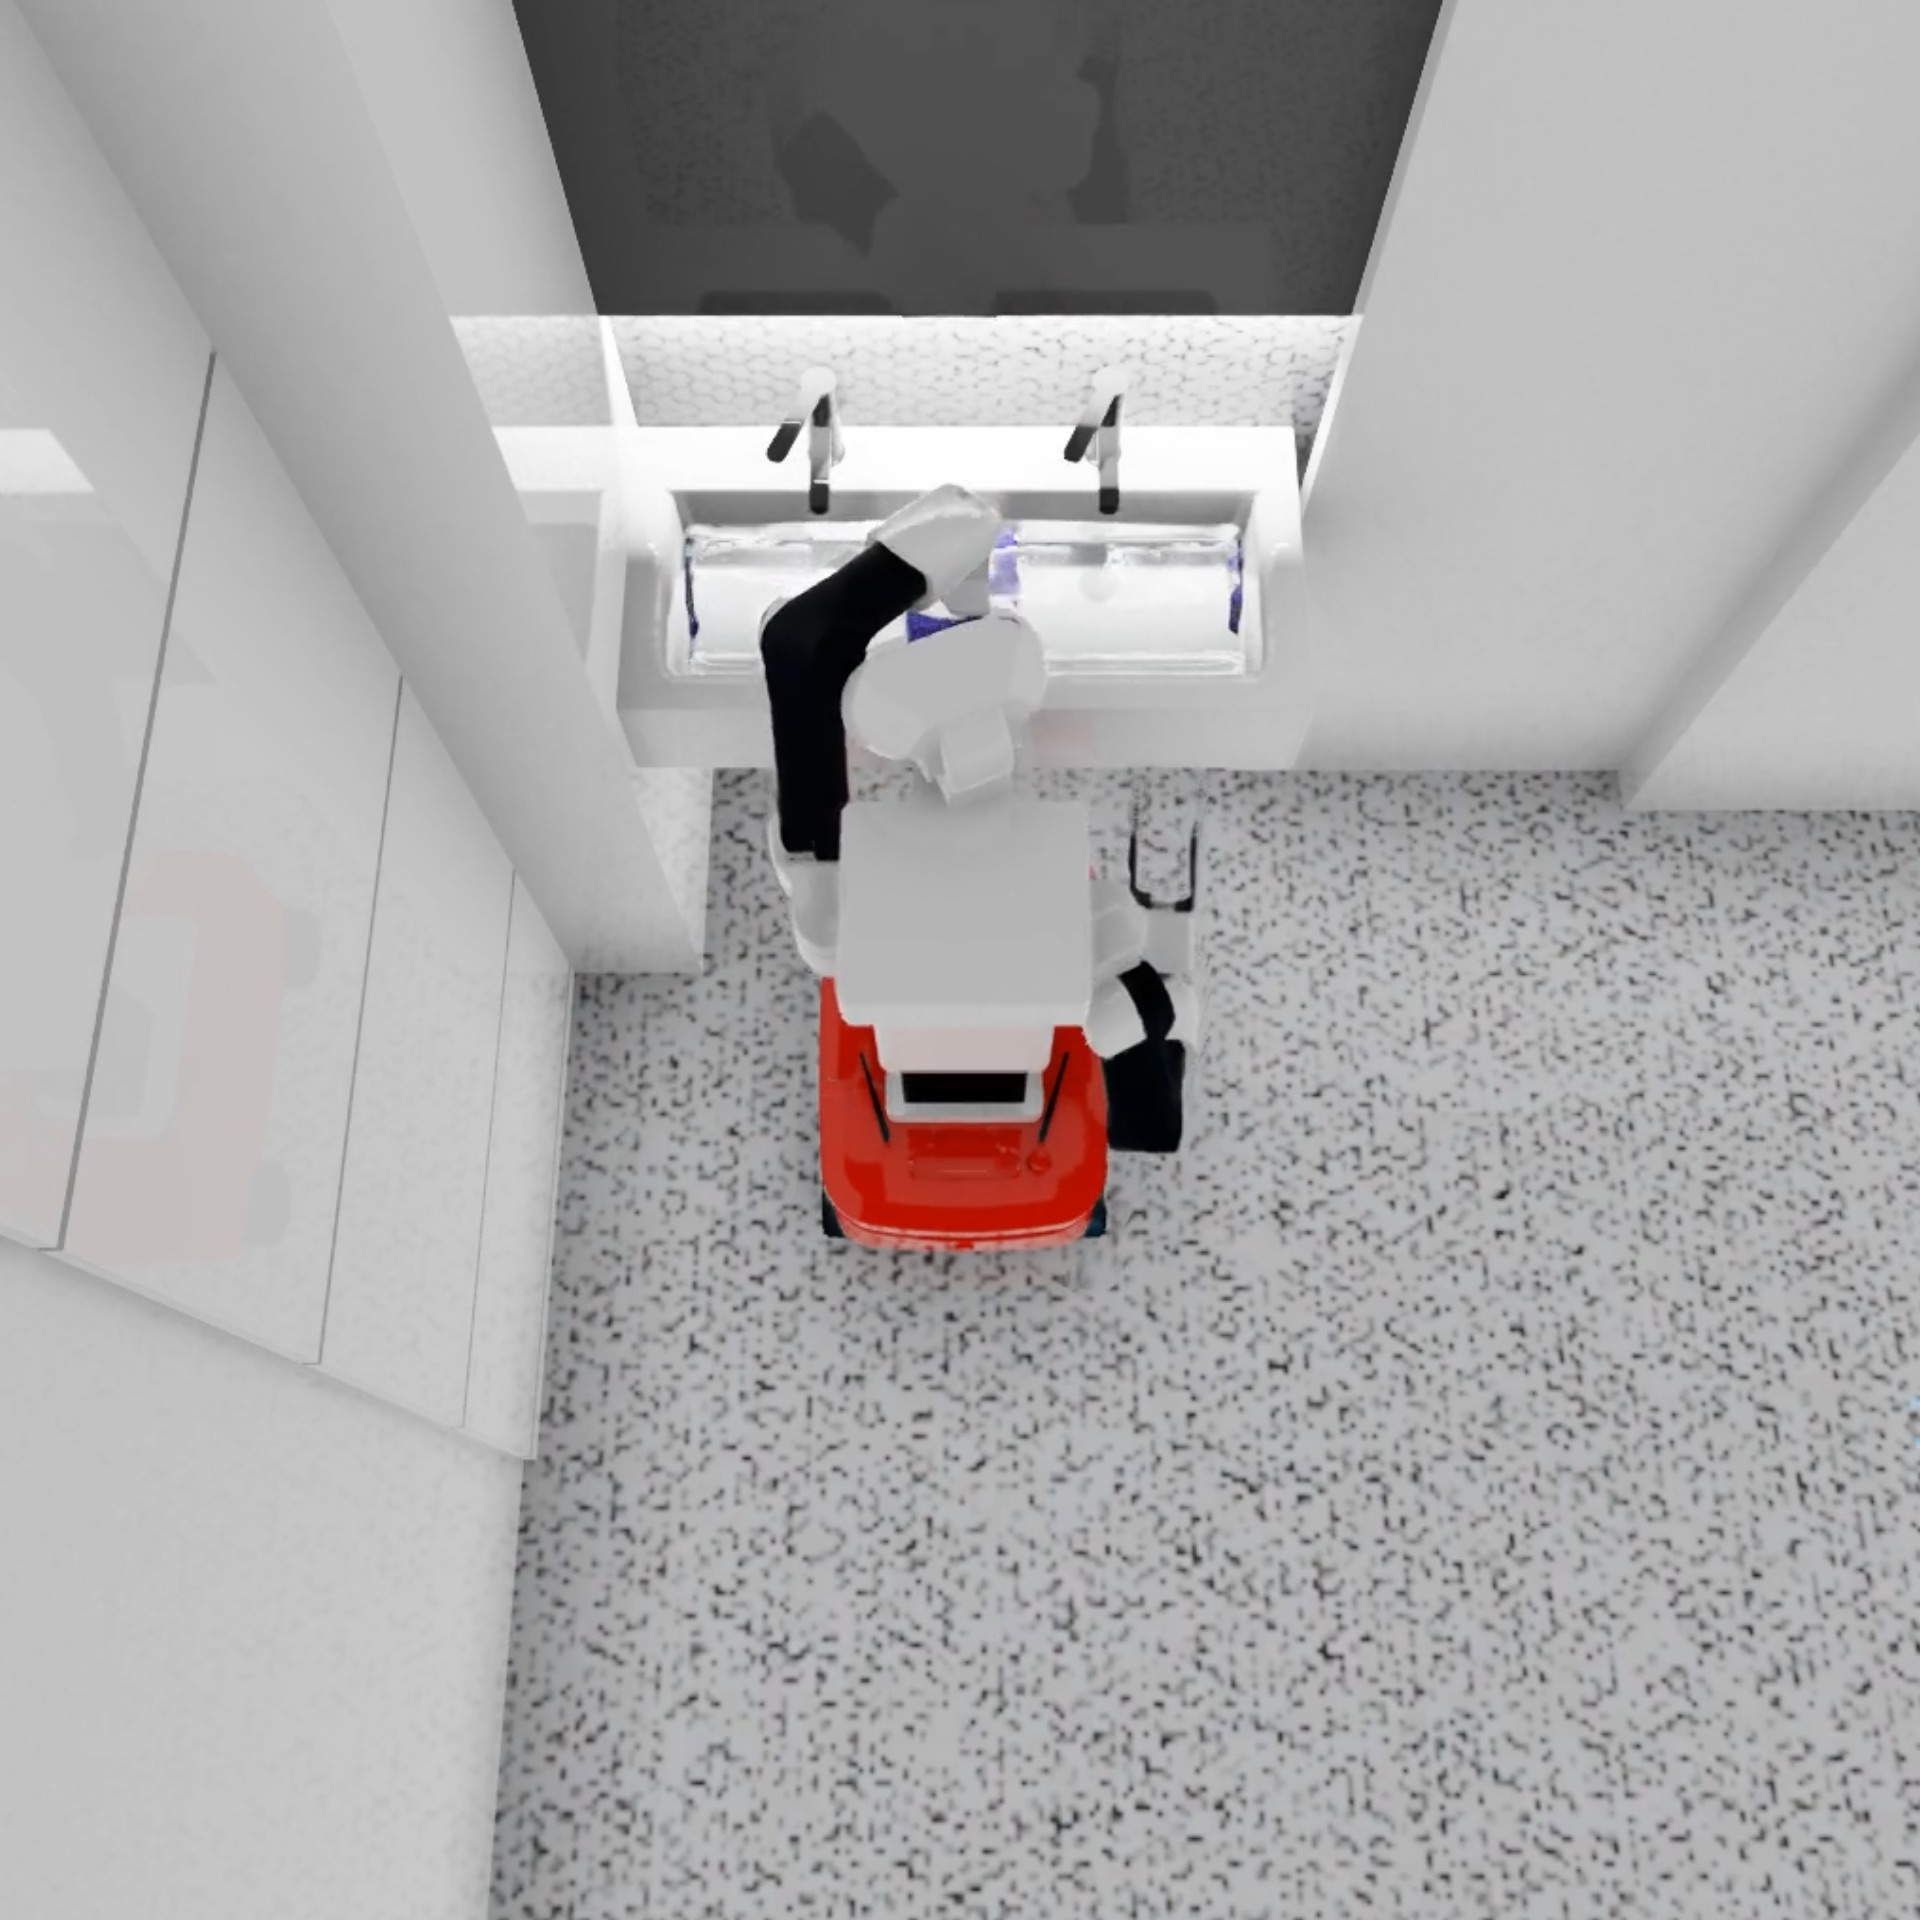
\includegraphics[trim=0 200 0 100,clip,width=0.3\linewidth]{figures/baseline_appendix/dip_2}&
%         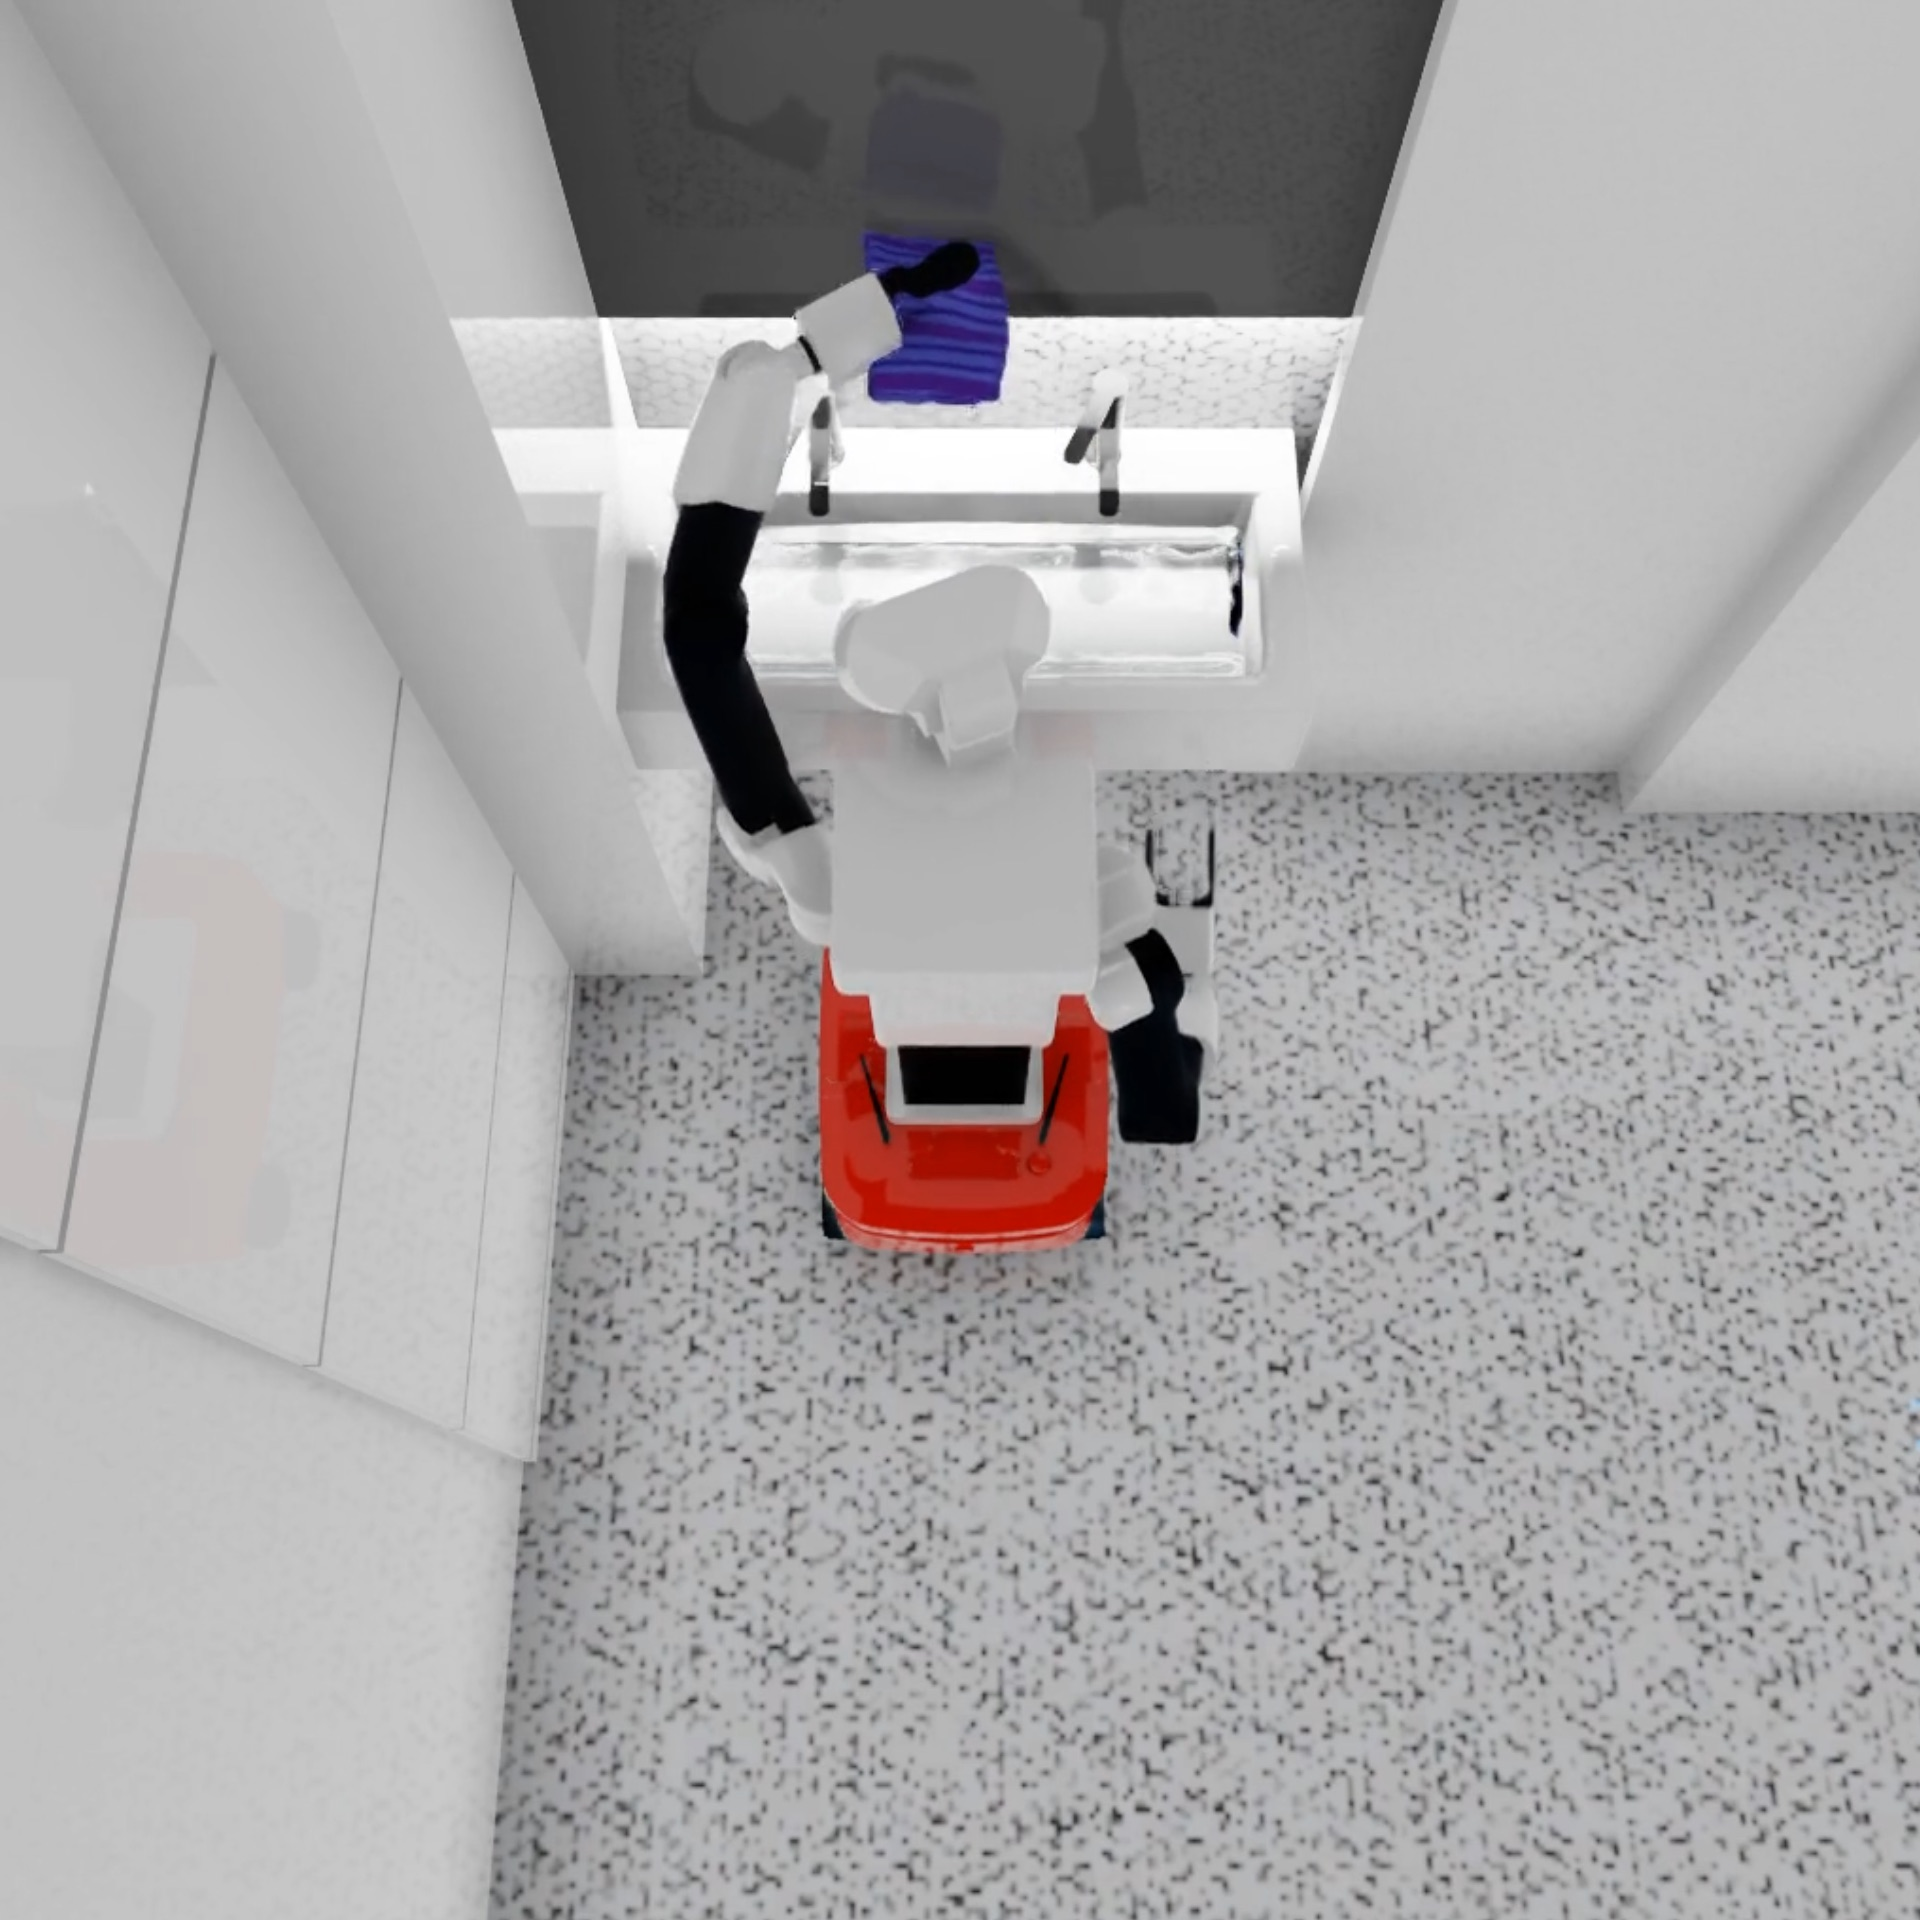
\includegraphics[trim=0 200 0 100,clip,width=0.3\linewidth]{figures/baseline_appendix/dip_3}\\
%         & e) \texttt{dip}  & \\
%         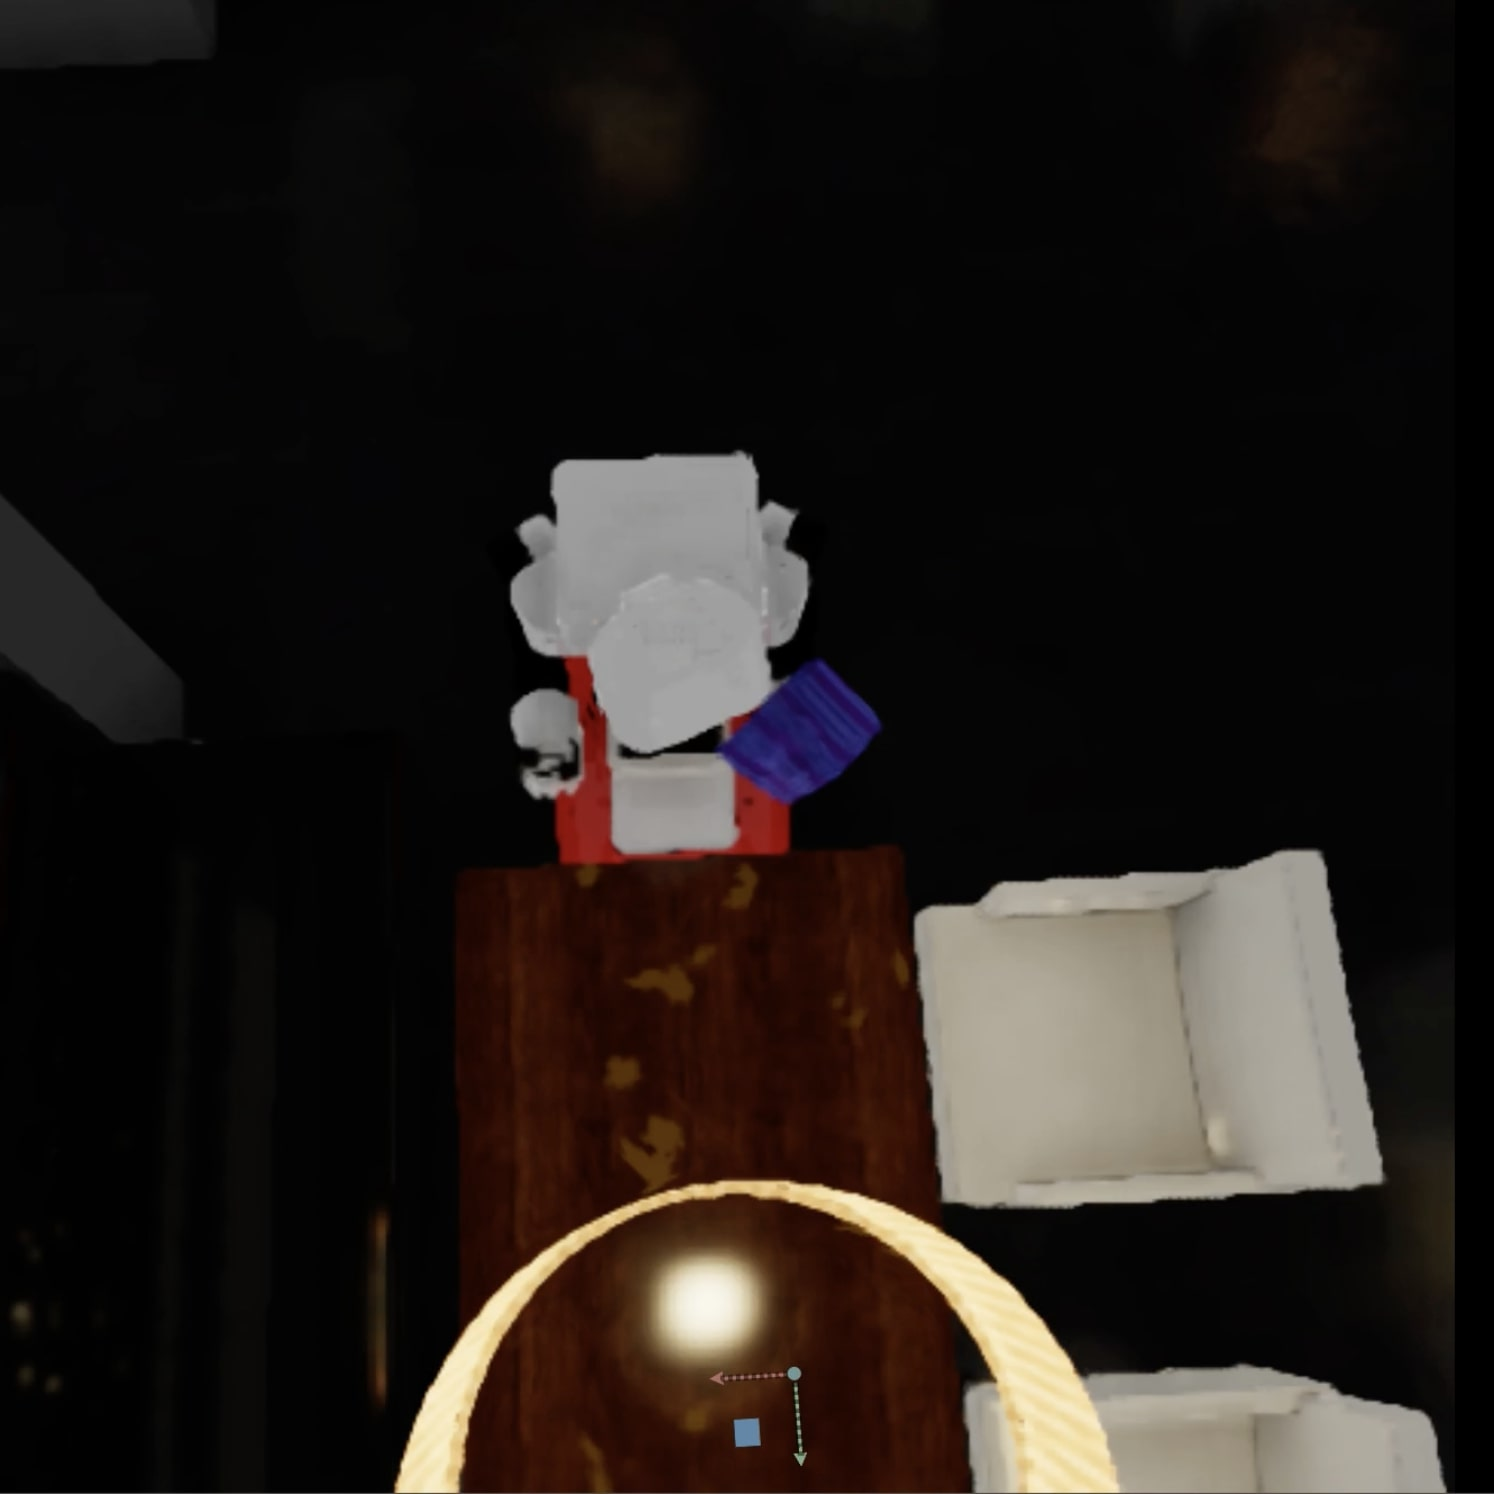
\includegraphics[trim=0 100 0 200,clip,width=0.3\linewidth]{figures/baseline_appendix/wipe_1}&
%         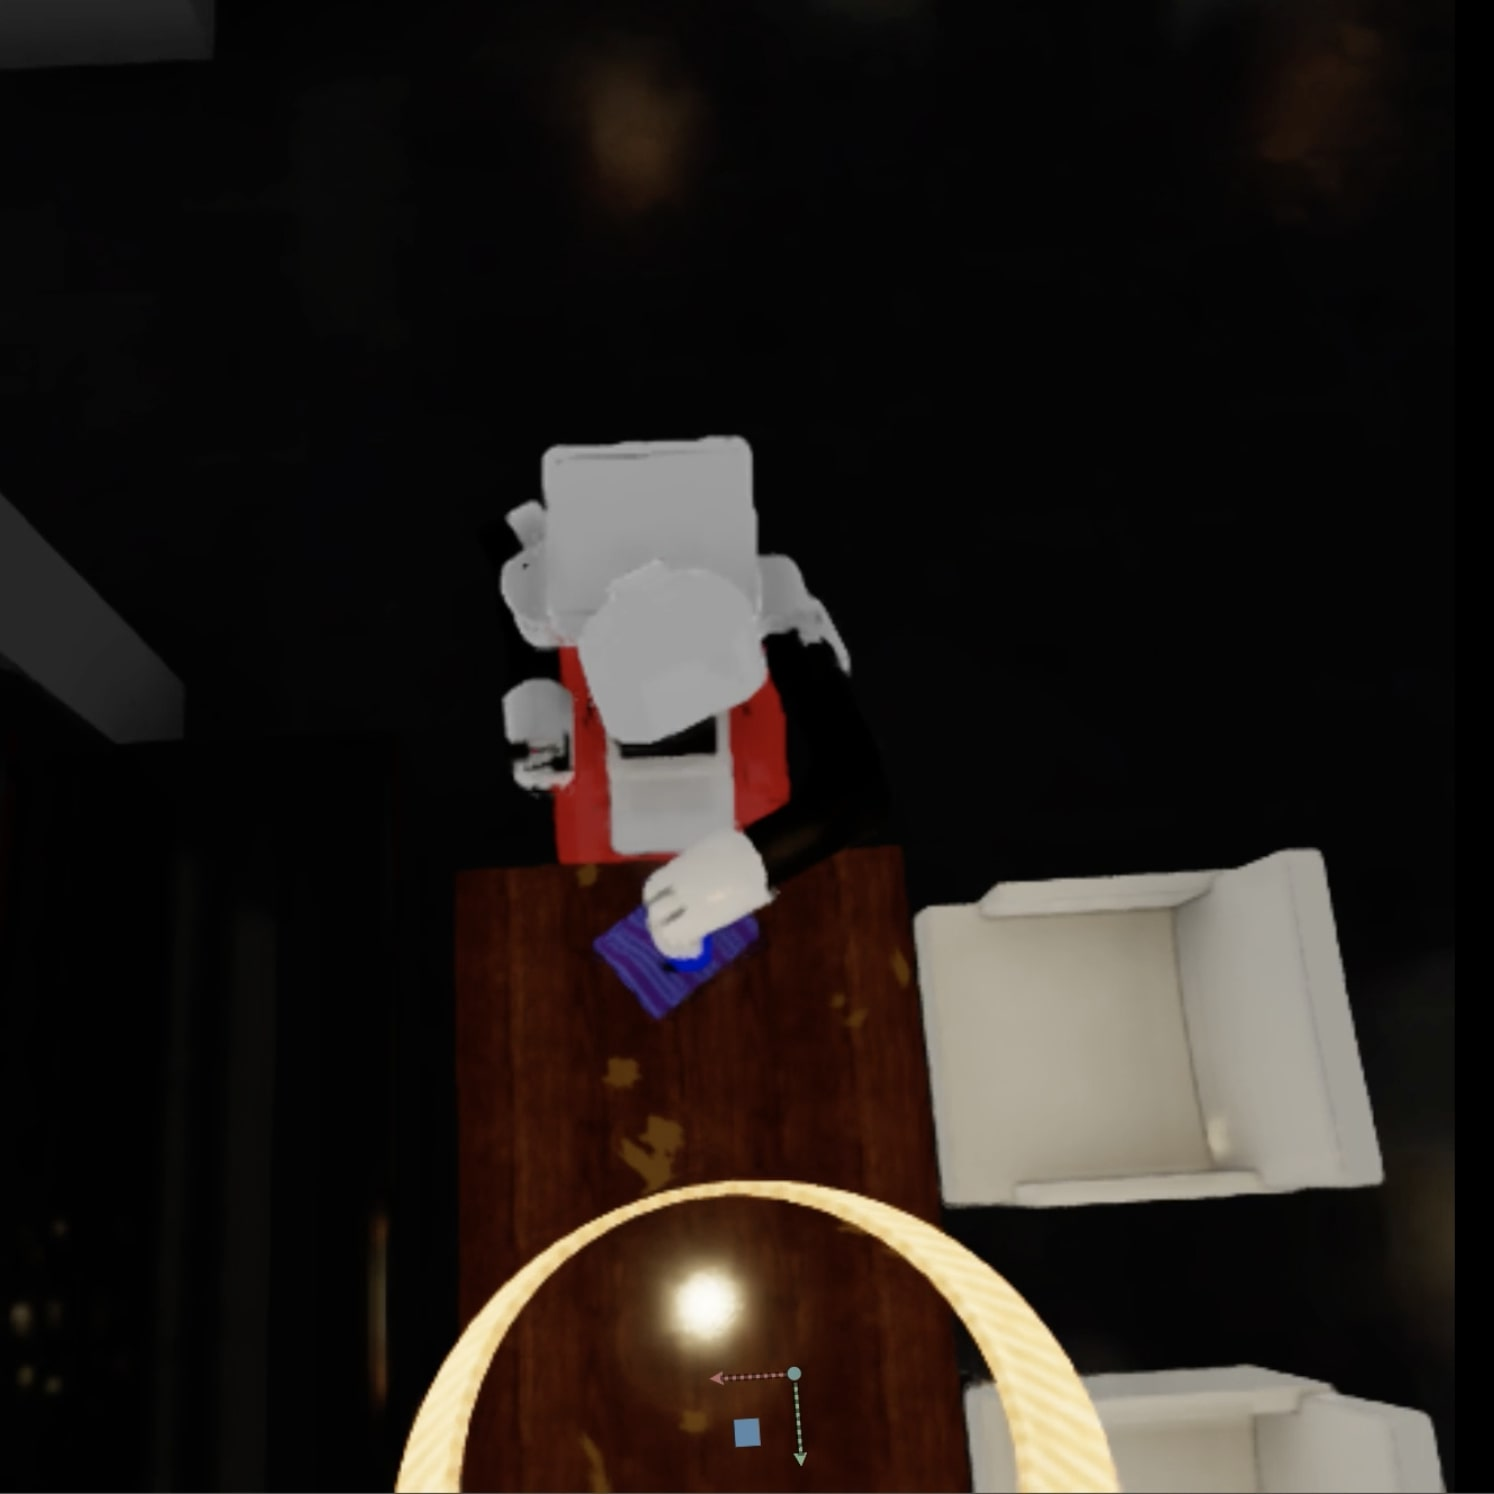
\includegraphics[trim=0 100 0 200,clip,width=0.3\linewidth]{figures/baseline_appendix/wipe_2}&
%         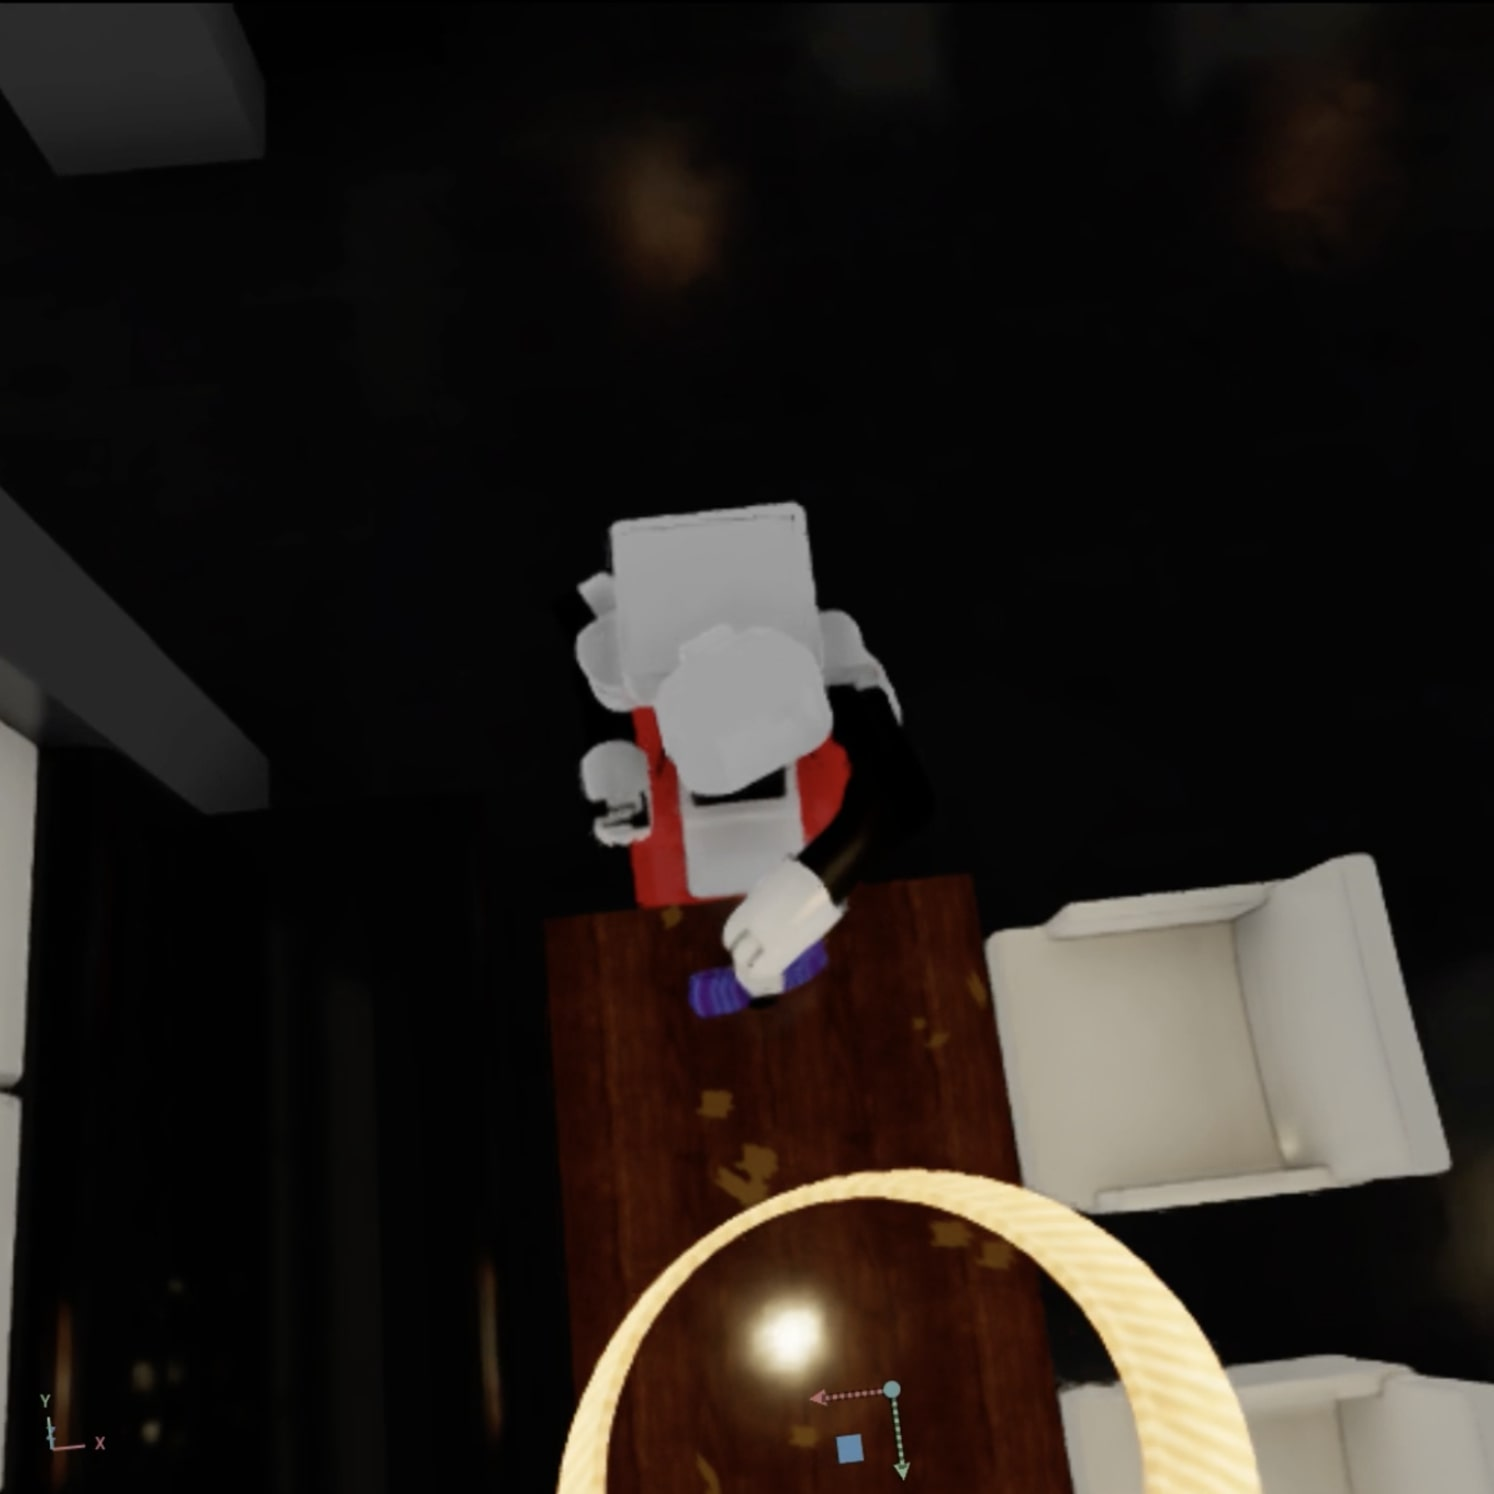
\includegraphics[trim=0 100 0 200,clip,width=0.3\linewidth]{figures/baseline_appendix/wipe_3}\\
%         & f) \texttt{wipe}  & \\
%     \end{tabular}
%     \caption{Overview of all the high level planner actions with the pre-conditions (right), post-conditions (left), and an intermediate state when executing the action.
%     % \roberto{consider taking the images of wipe with more lights, it is hard to see. and the robot is gone in the last image}
%     }
%     \label{fig:appendix_high_level_planner}
% \end{figure}

\begin{figure}[h!]
\centering
\begin{subfigure}[t]{0.8\textwidth}{\centering
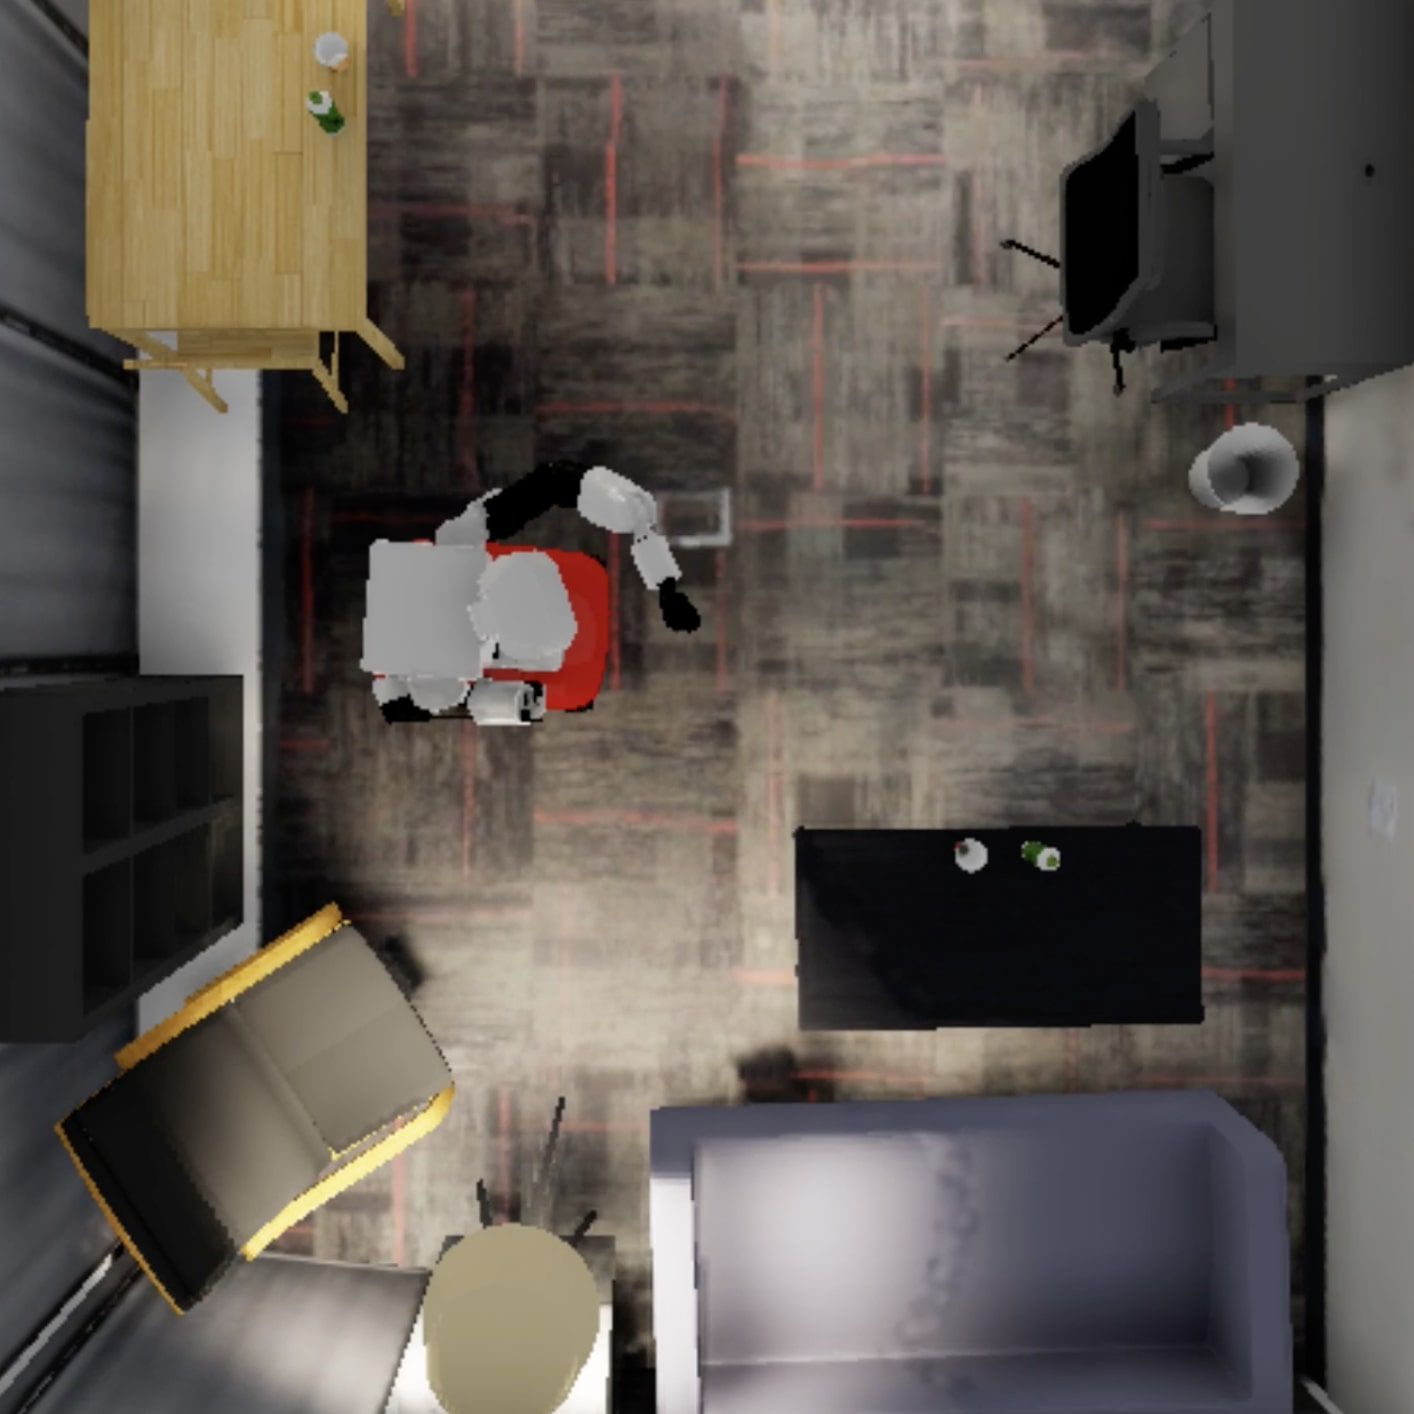
\includegraphics[trim=0 200 0 200,clip,width=0.33\linewidth]{figures/baseline_appendix/navigate_to_1}%
\hfill%
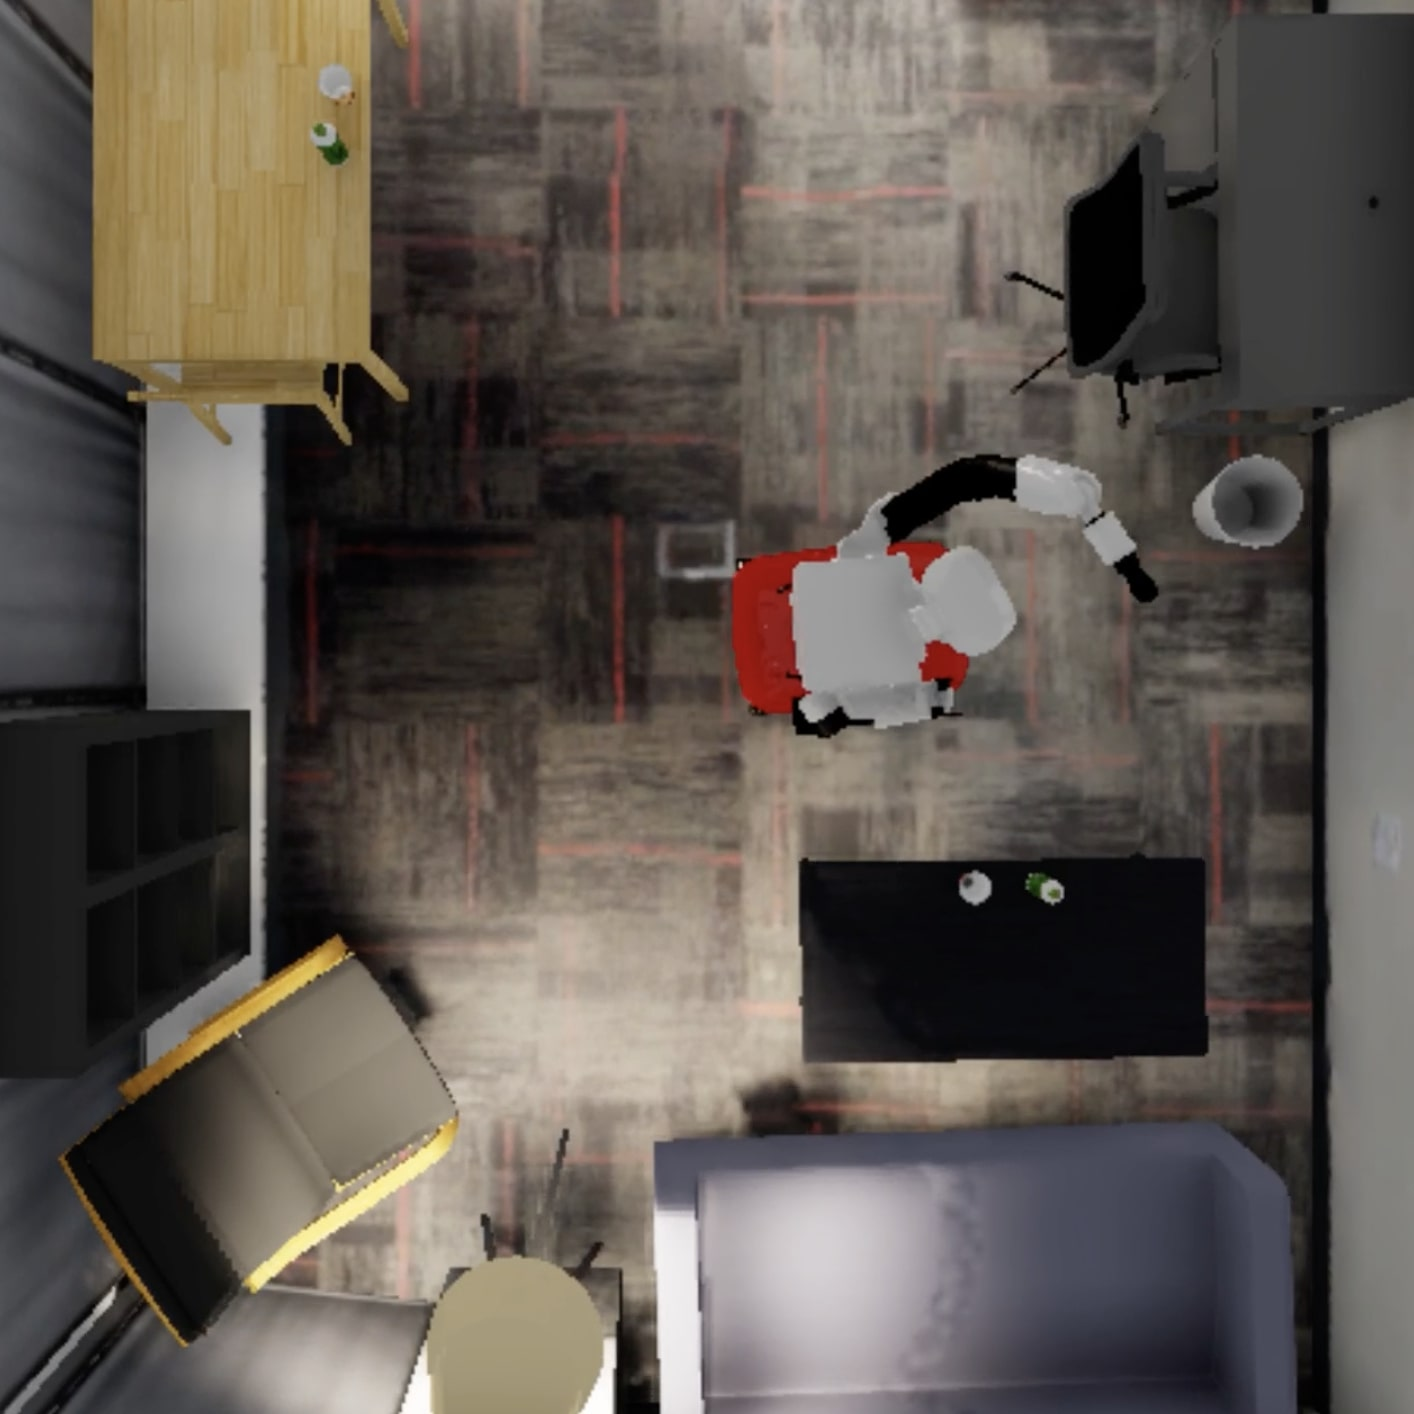
\includegraphics[trim=0 200 0 200,clip,width=0.33\linewidth]{figures/baseline_appendix/navigate_to_2}%
\hfill%
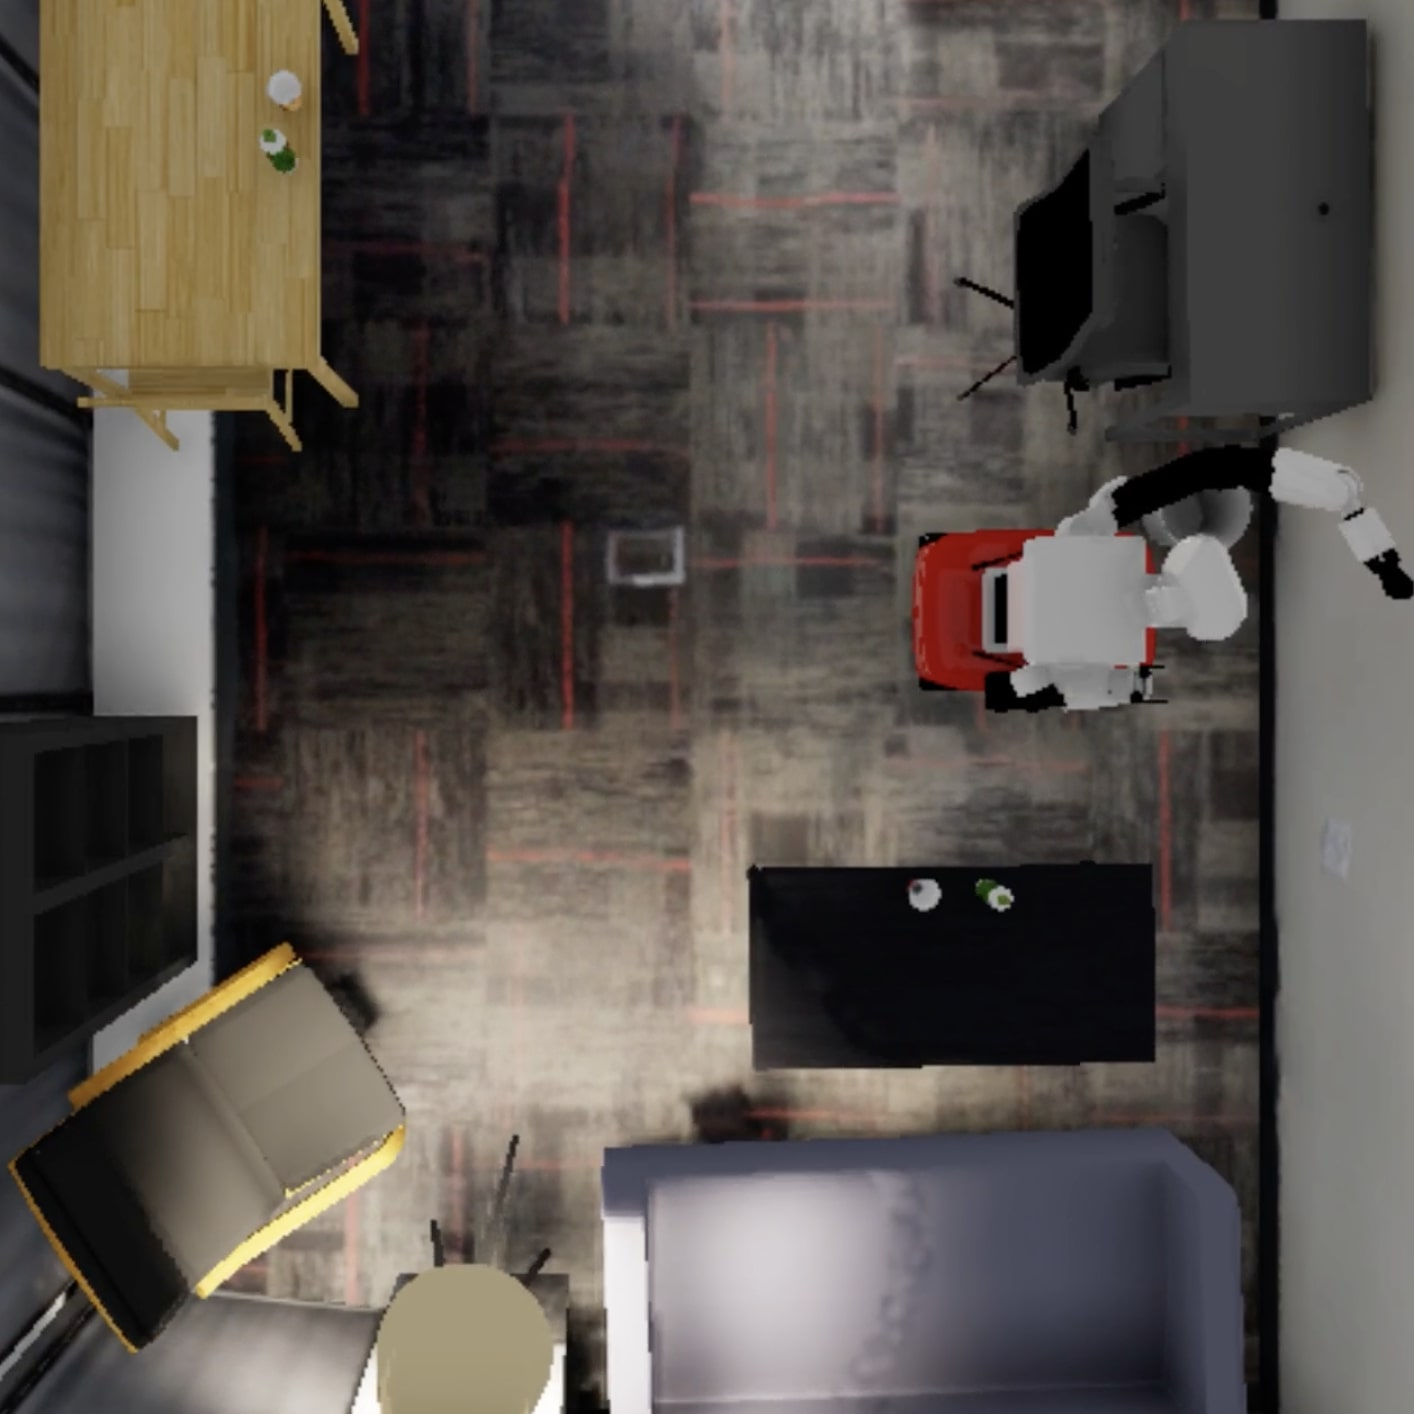
\includegraphics[trim=0 200 0 200,clip,width=0.33\linewidth]{figures/baseline_appendix/navigate_to_3}%
}
\vspace{-5pt}
\caption{\texttt{navigate}}
\vspace{10pt}
\end{subfigure}
\begin{subfigure}[t]{0.8\textwidth}{\centering
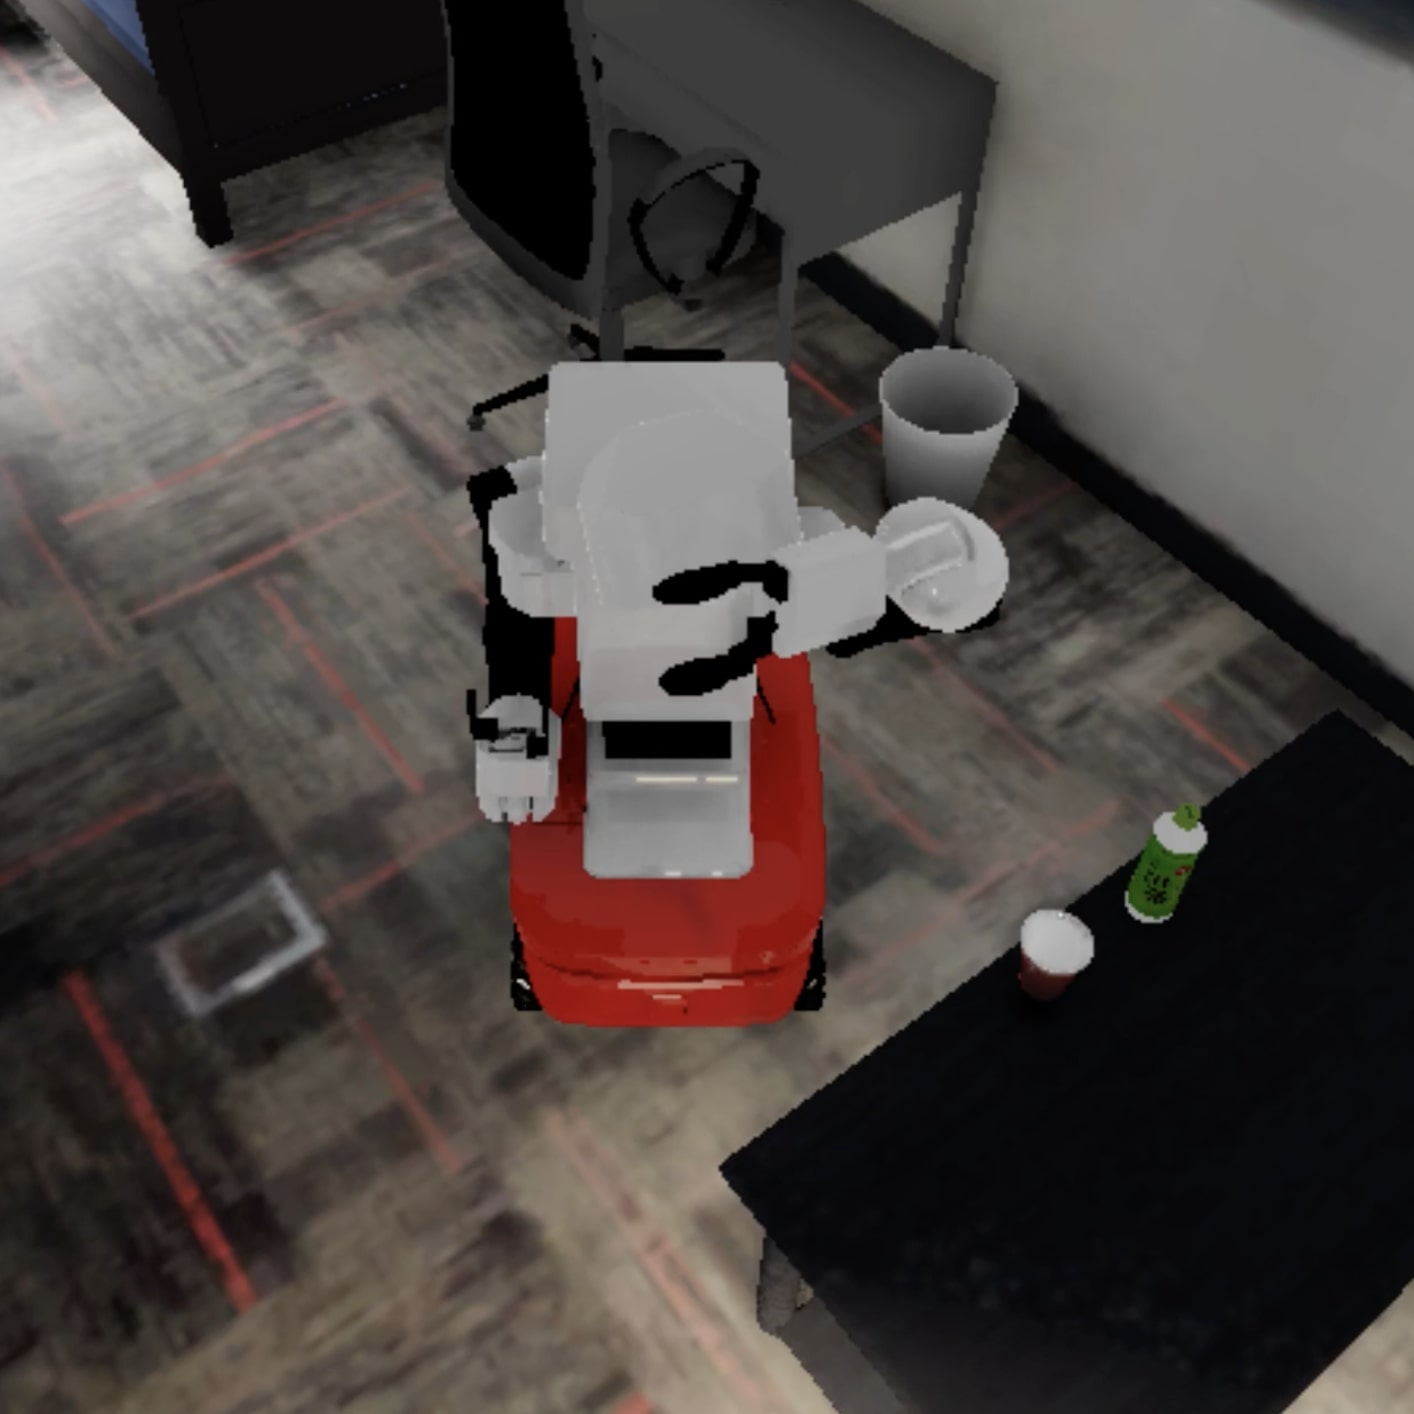
\includegraphics[trim=0 200 0 200,clip,width=0.33\linewidth]{figures/baseline_appendix/pick_1}%
\hfill%
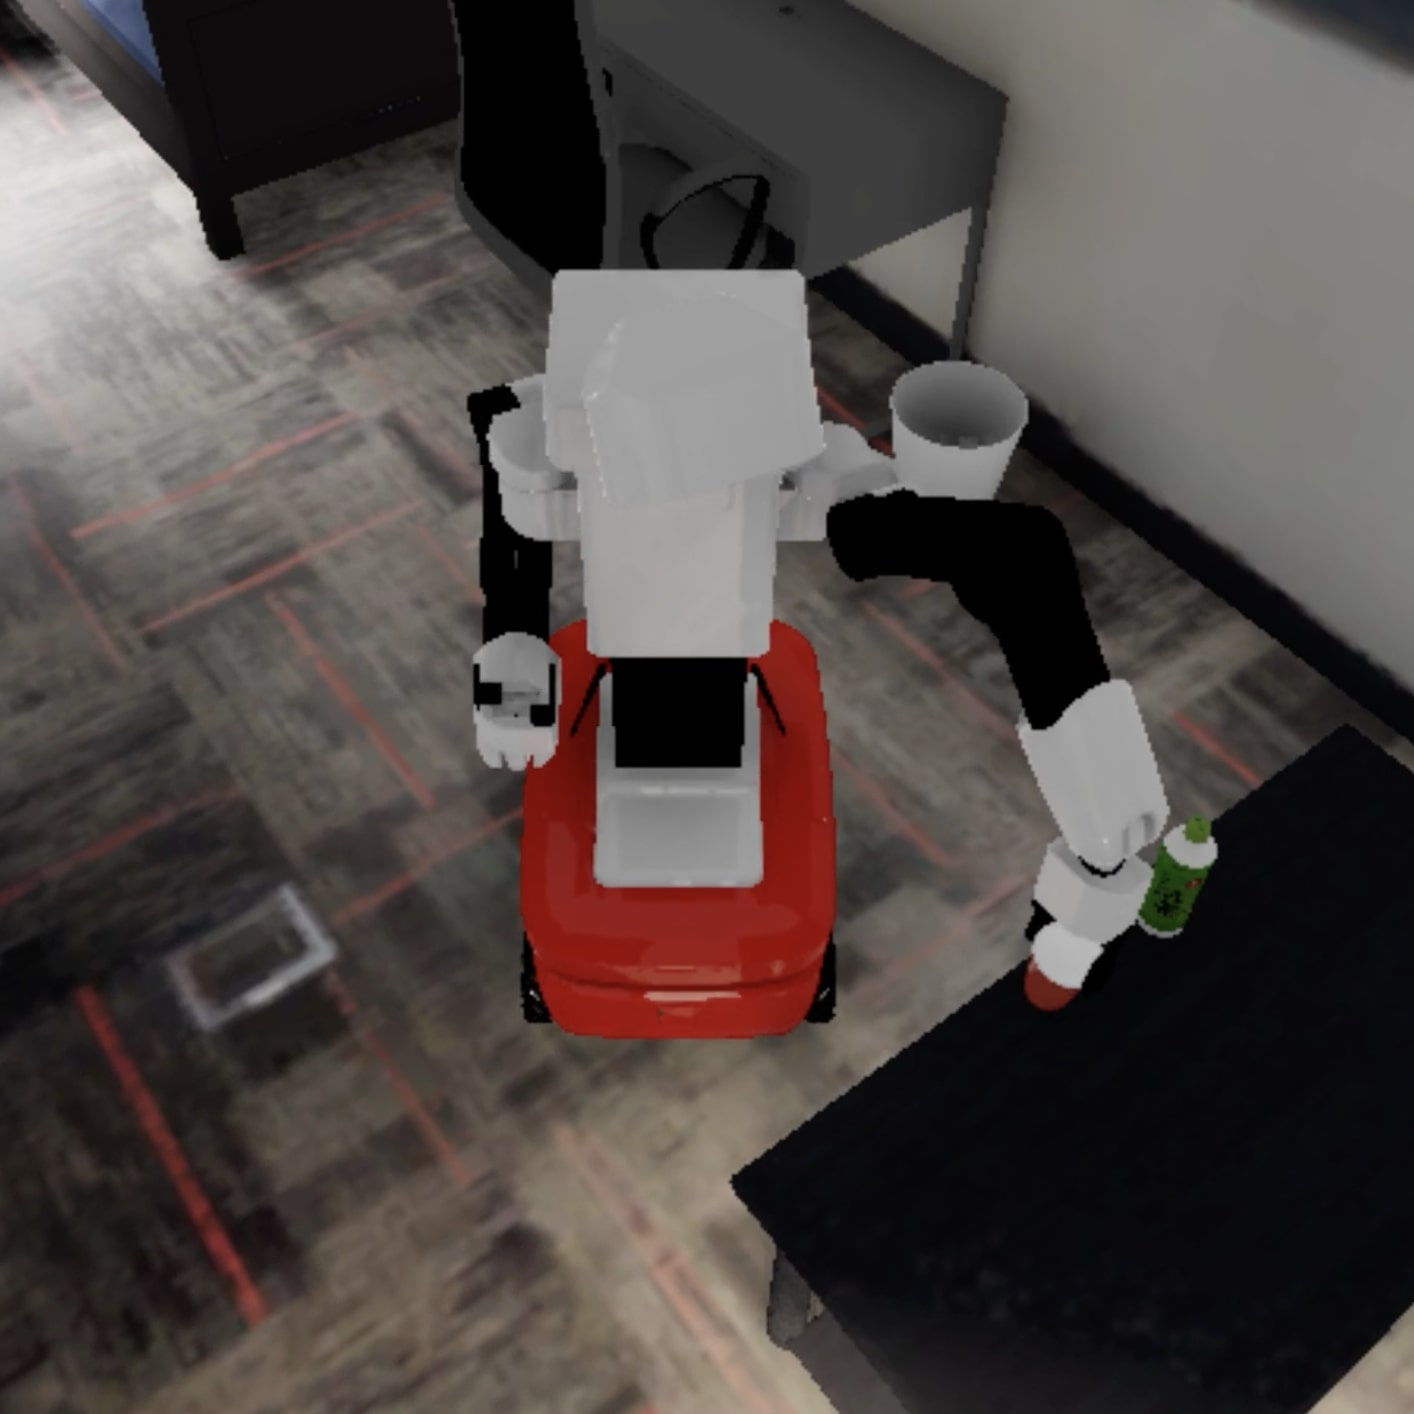
\includegraphics[trim=0 200 0 200,clip,width=0.33\linewidth]{figures/baseline_appendix/pick_2}%
\hfill%
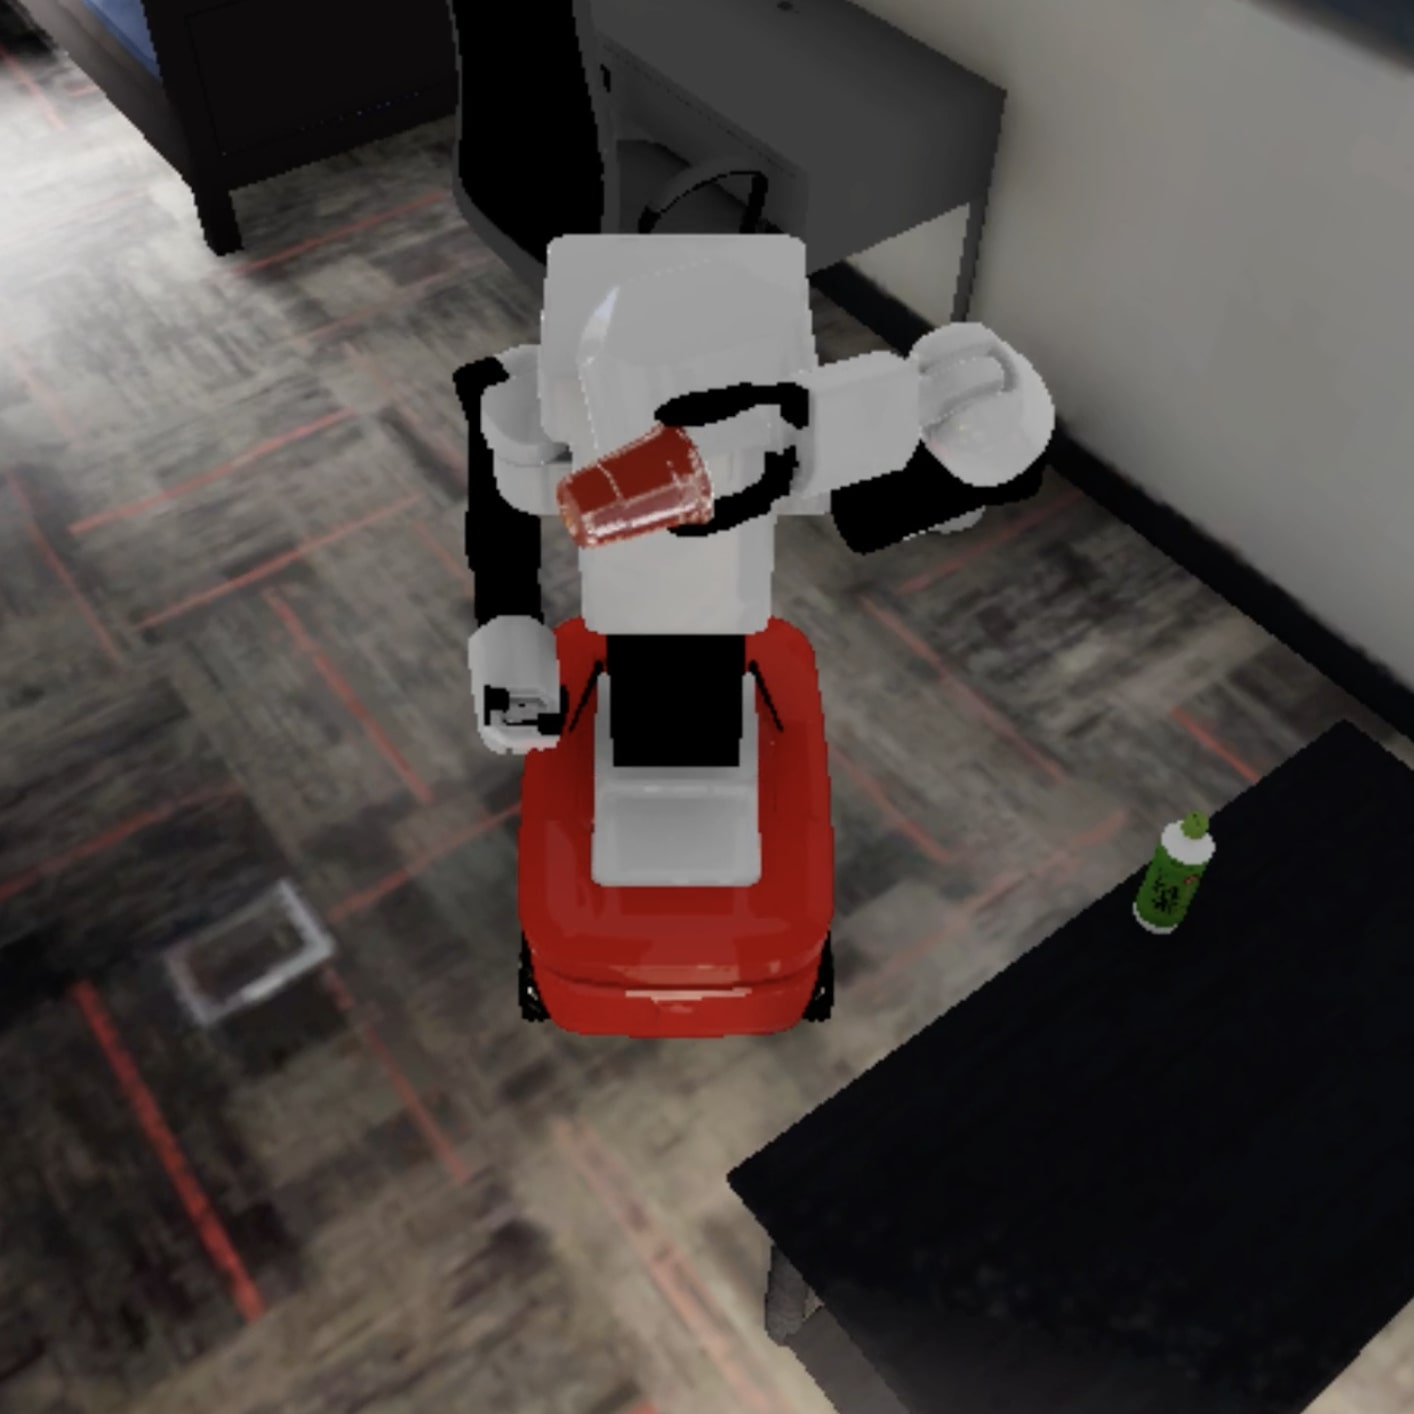
\includegraphics[trim=0 200 0 200,clip,width=0.33\linewidth]{figures/baseline_appendix/pick_3}
}%
\vspace{-5pt}%
\caption{\texttt{pick}}%
\vspace{10pt}%
\end{subfigure}
\begin{subfigure}[t]{0.8\textwidth}{\centering
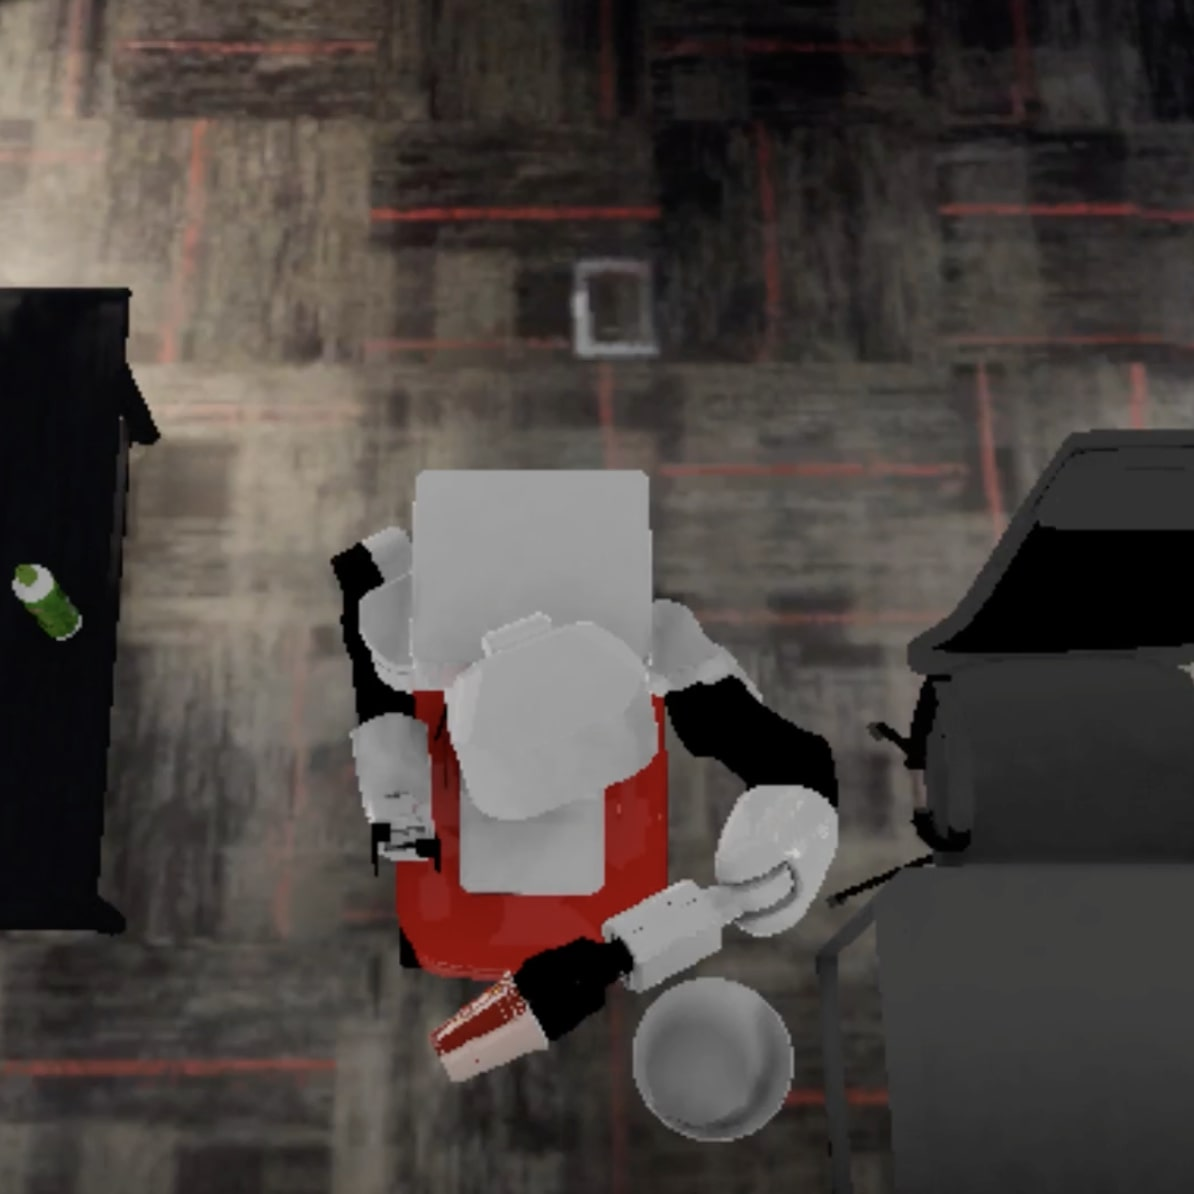
\includegraphics[trim=0 0 0 250,clip, width=0.33\linewidth]{figures/baseline_appendix/place_1}%
\hfill%
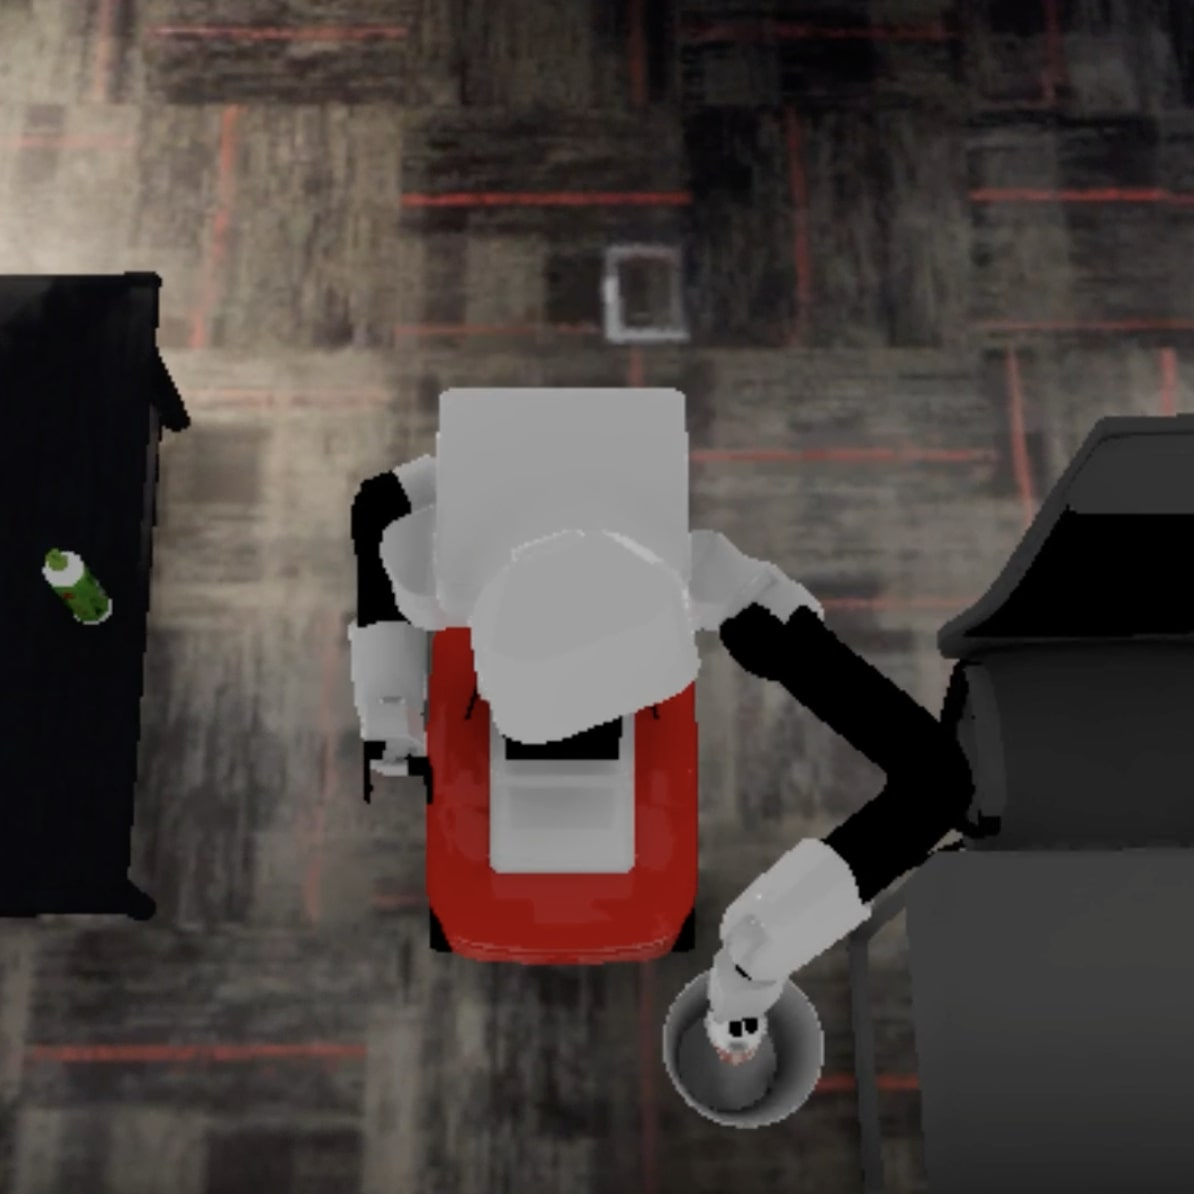
\includegraphics[trim=0 0 0 250,clip,width=0.33\linewidth]{figures/baseline_appendix/place_2}%
\hfill%
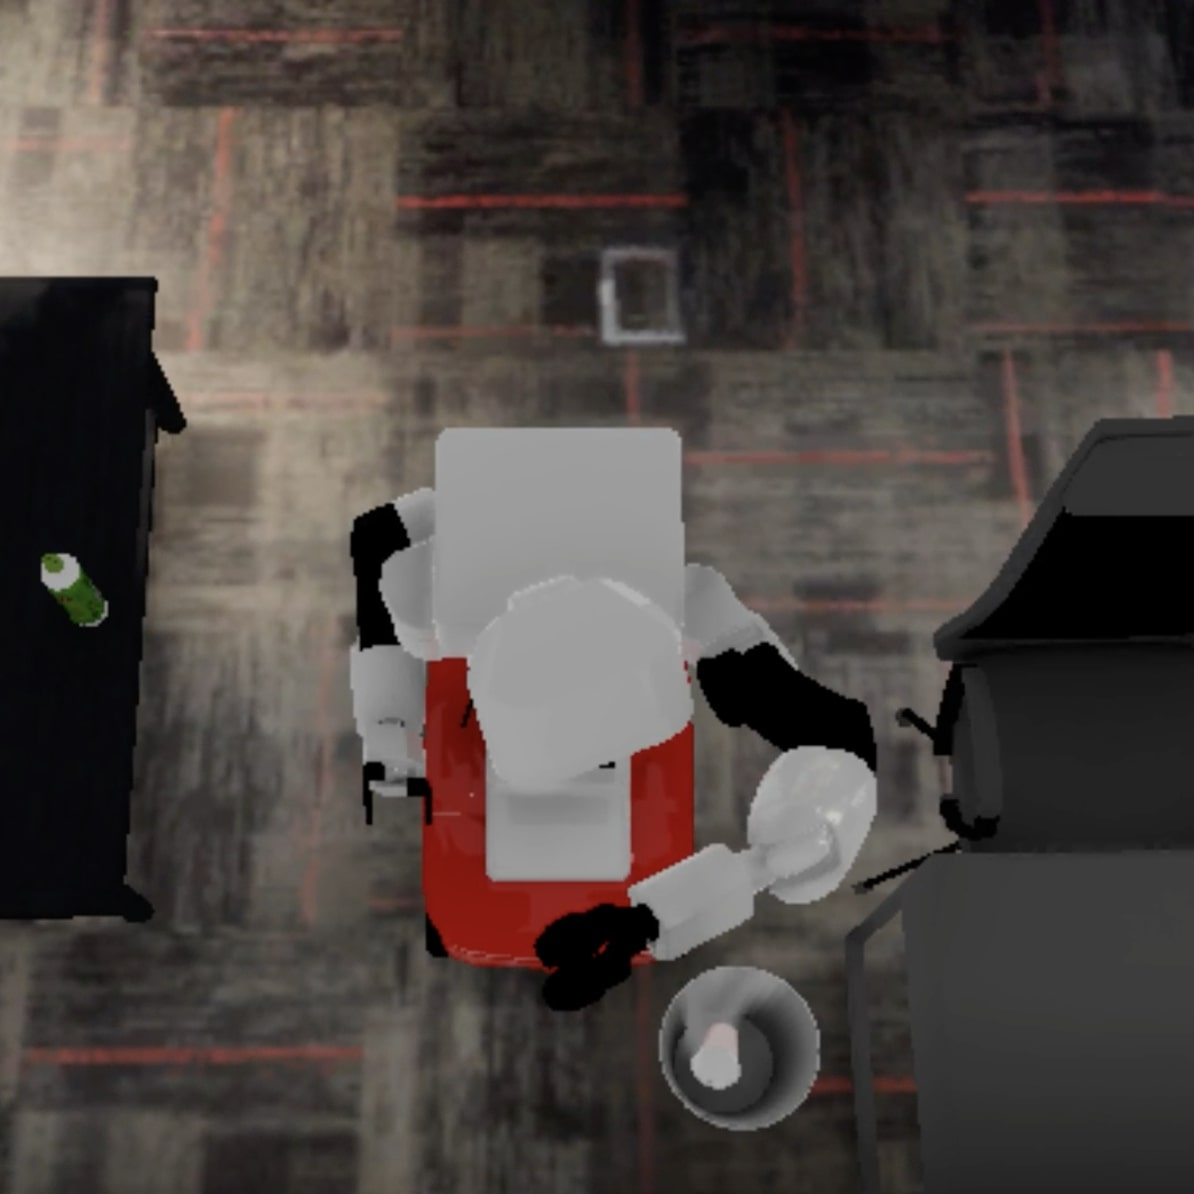
\includegraphics[trim=0 0 0 250,clip,width=0.33\linewidth]{figures/baseline_appendix/place_3}
}%
\vspace{-5pt}%
\caption{\texttt{place}}%
\vspace{10pt}%
\end{subfigure}
\begin{subfigure}[t]{0.8\textwidth}{\centering
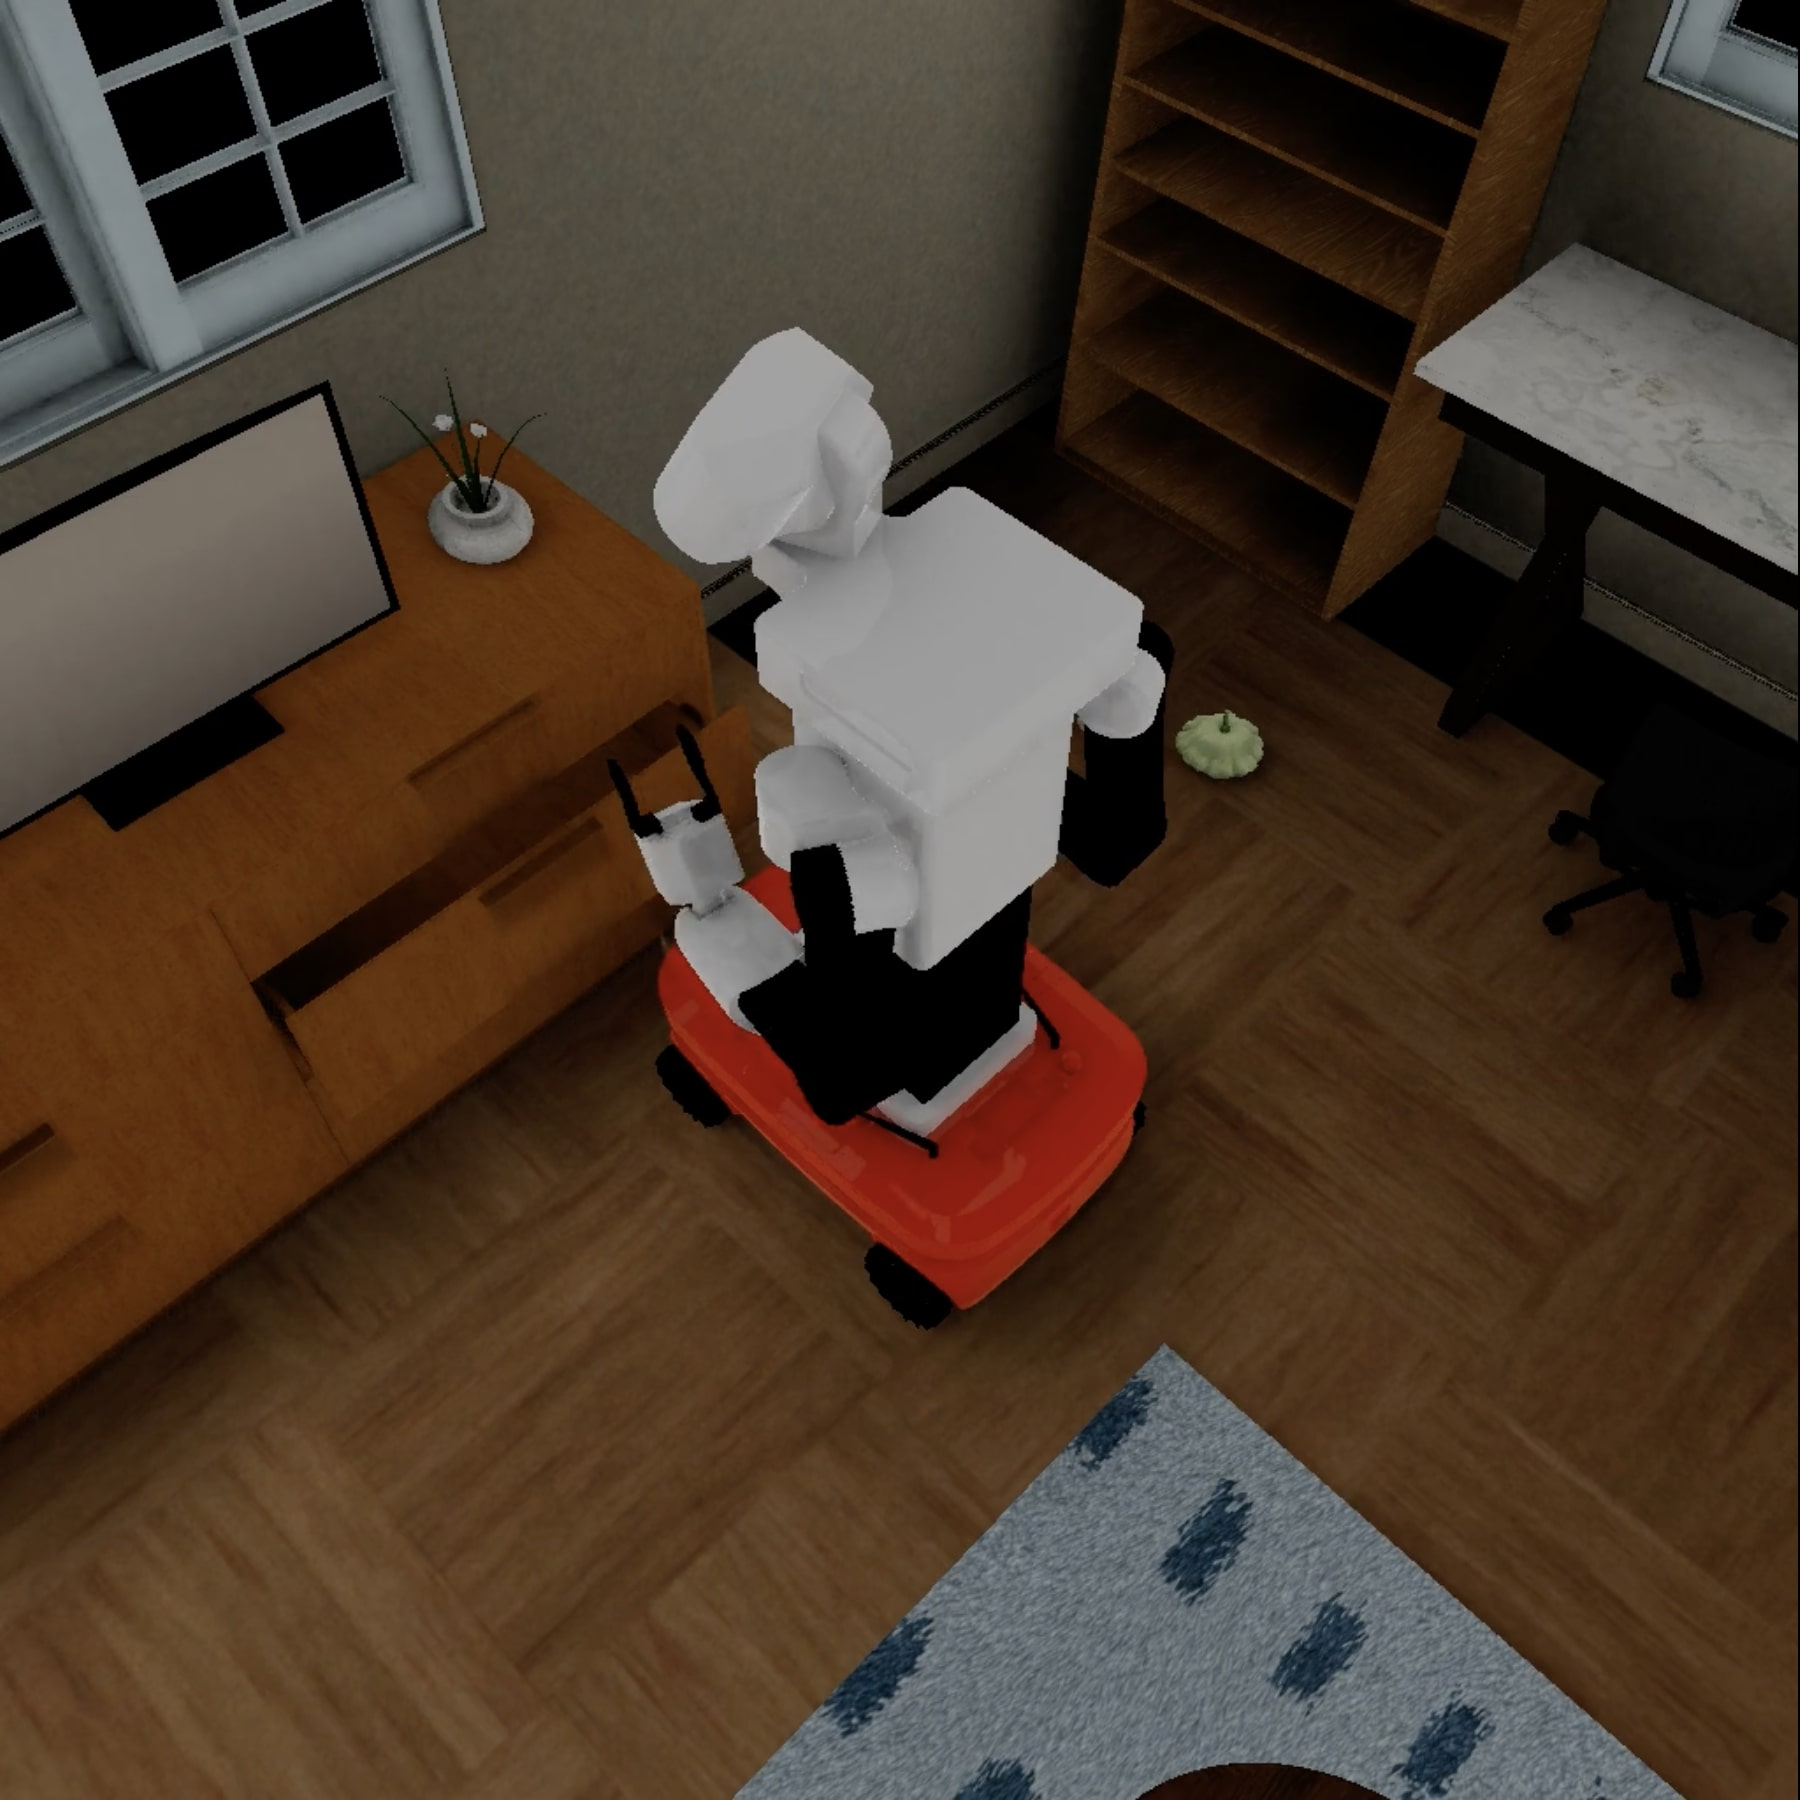
\includegraphics[trim=0 220 0 20,clip,width=0.33\linewidth]{figures/baseline_appendix/pull_1}%
\hfill%
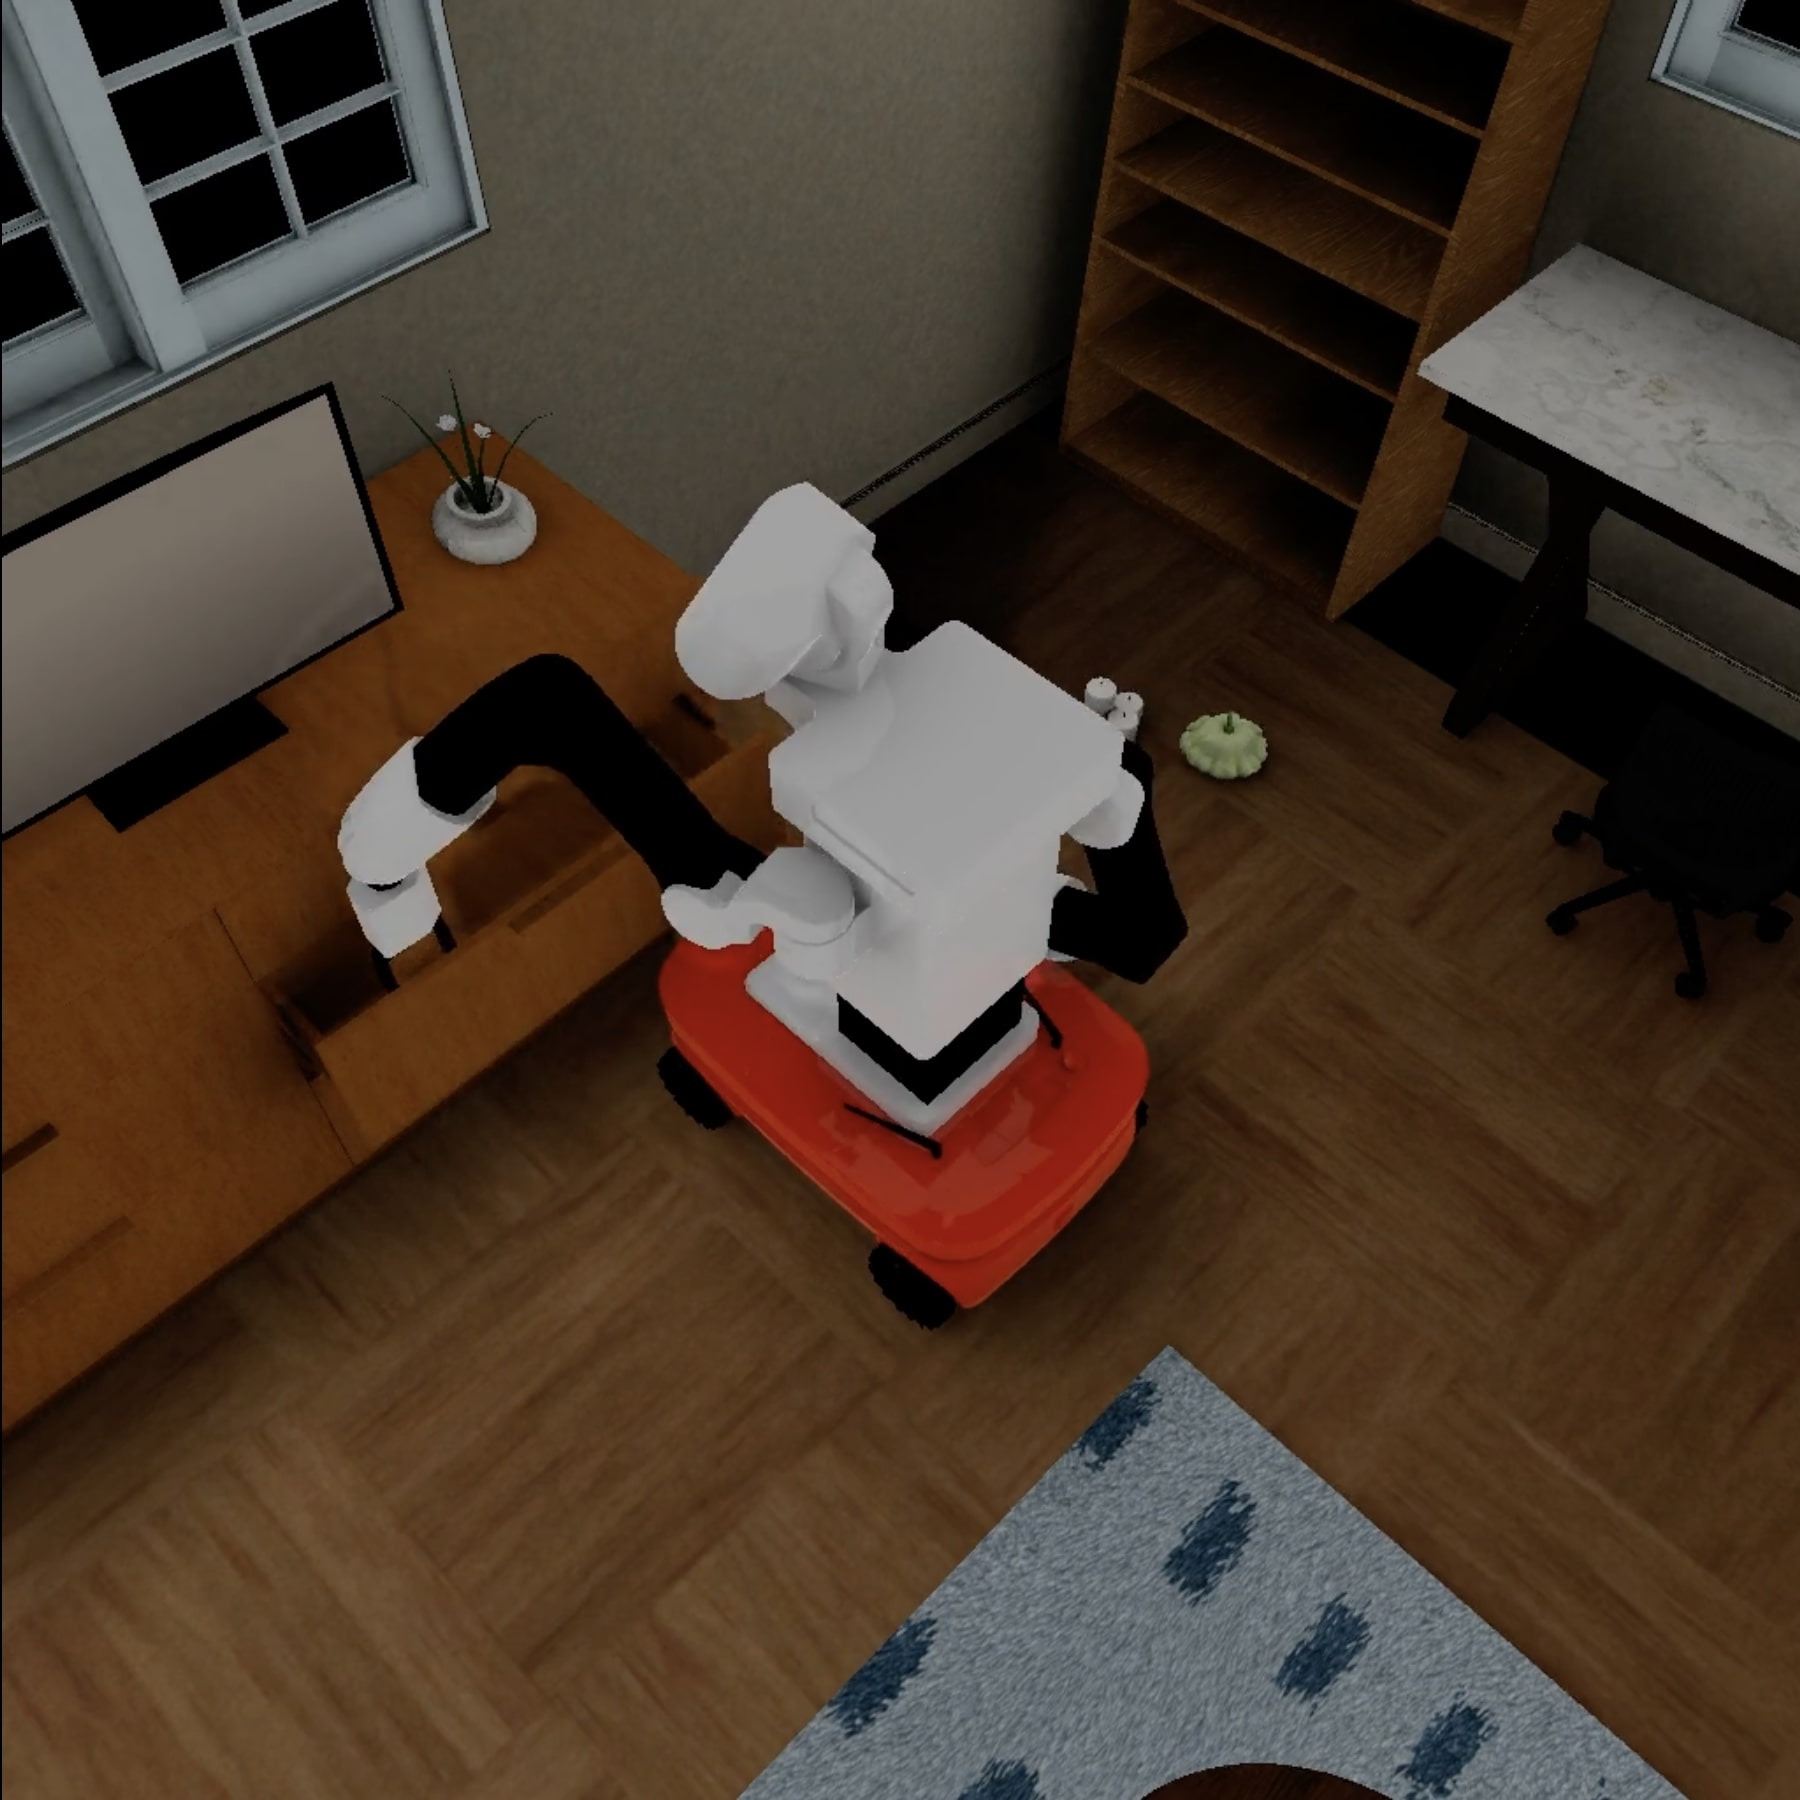
\includegraphics[trim=0 220 0 20,clip,width=0.33\linewidth]{figures/baseline_appendix/pull_2}%
\hfill%
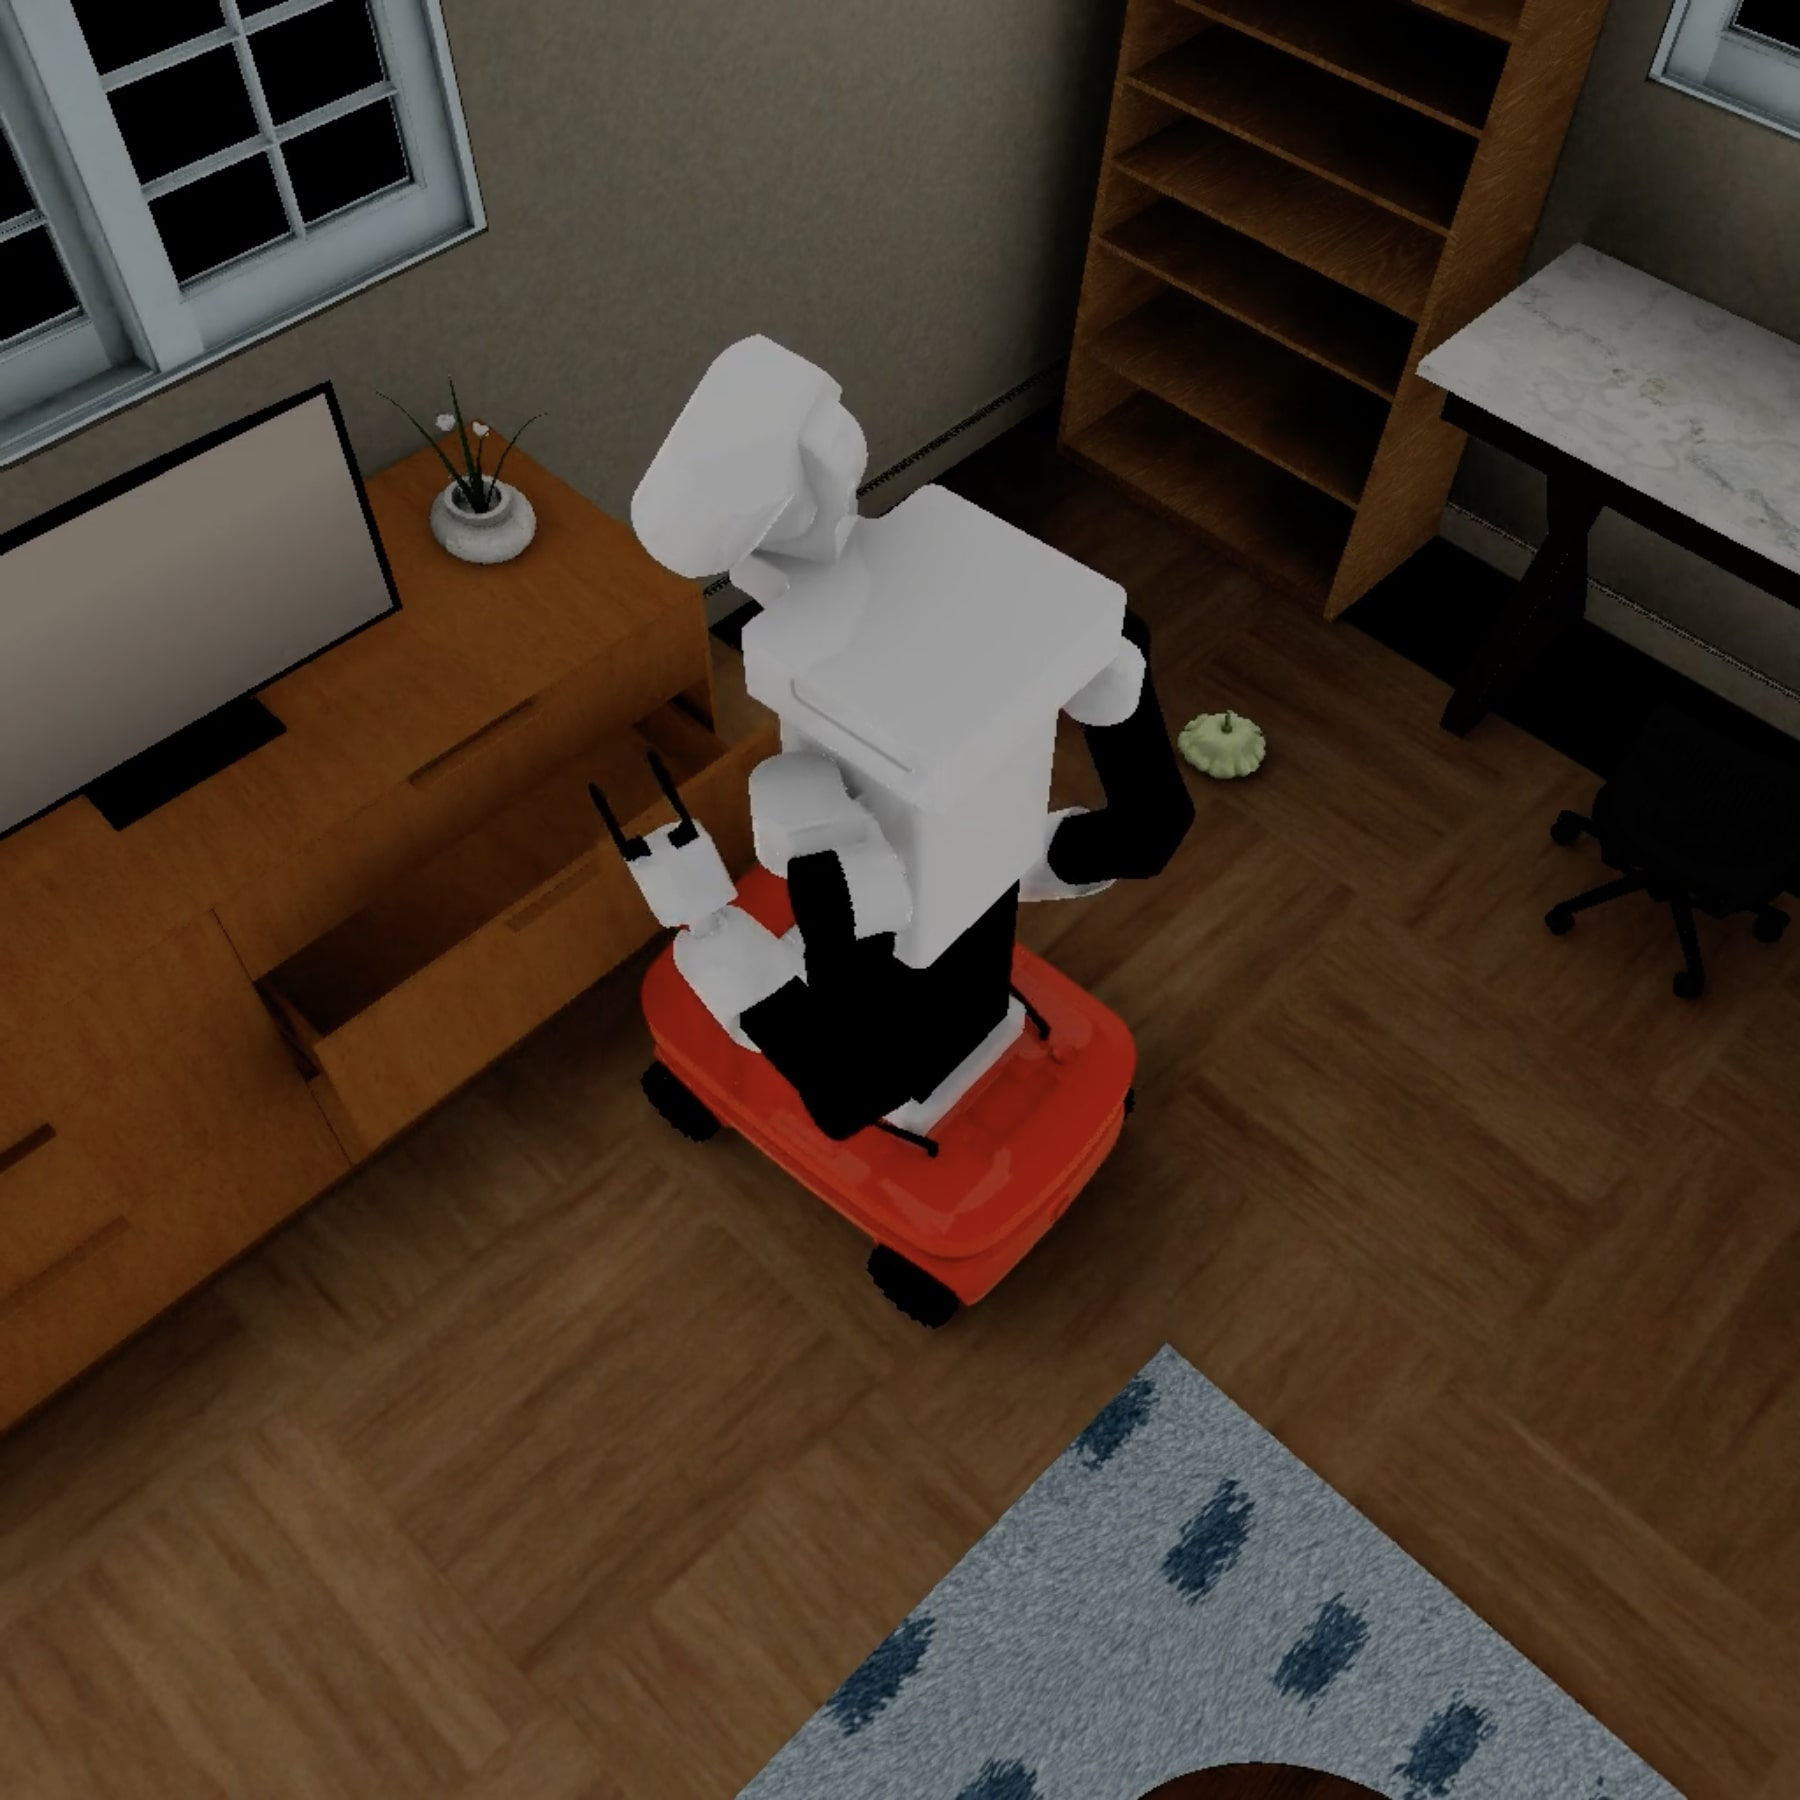
\includegraphics[trim=0 220 0 20,clip,width=0.33\linewidth]{figures/baseline_appendix/pull_3}
}%
\vspace{-5pt}
\caption{\texttt{push} (open)}
\vspace{10pt}
\end{subfigure}
\begin{subfigure}[t]{0.8\textwidth}{\centering
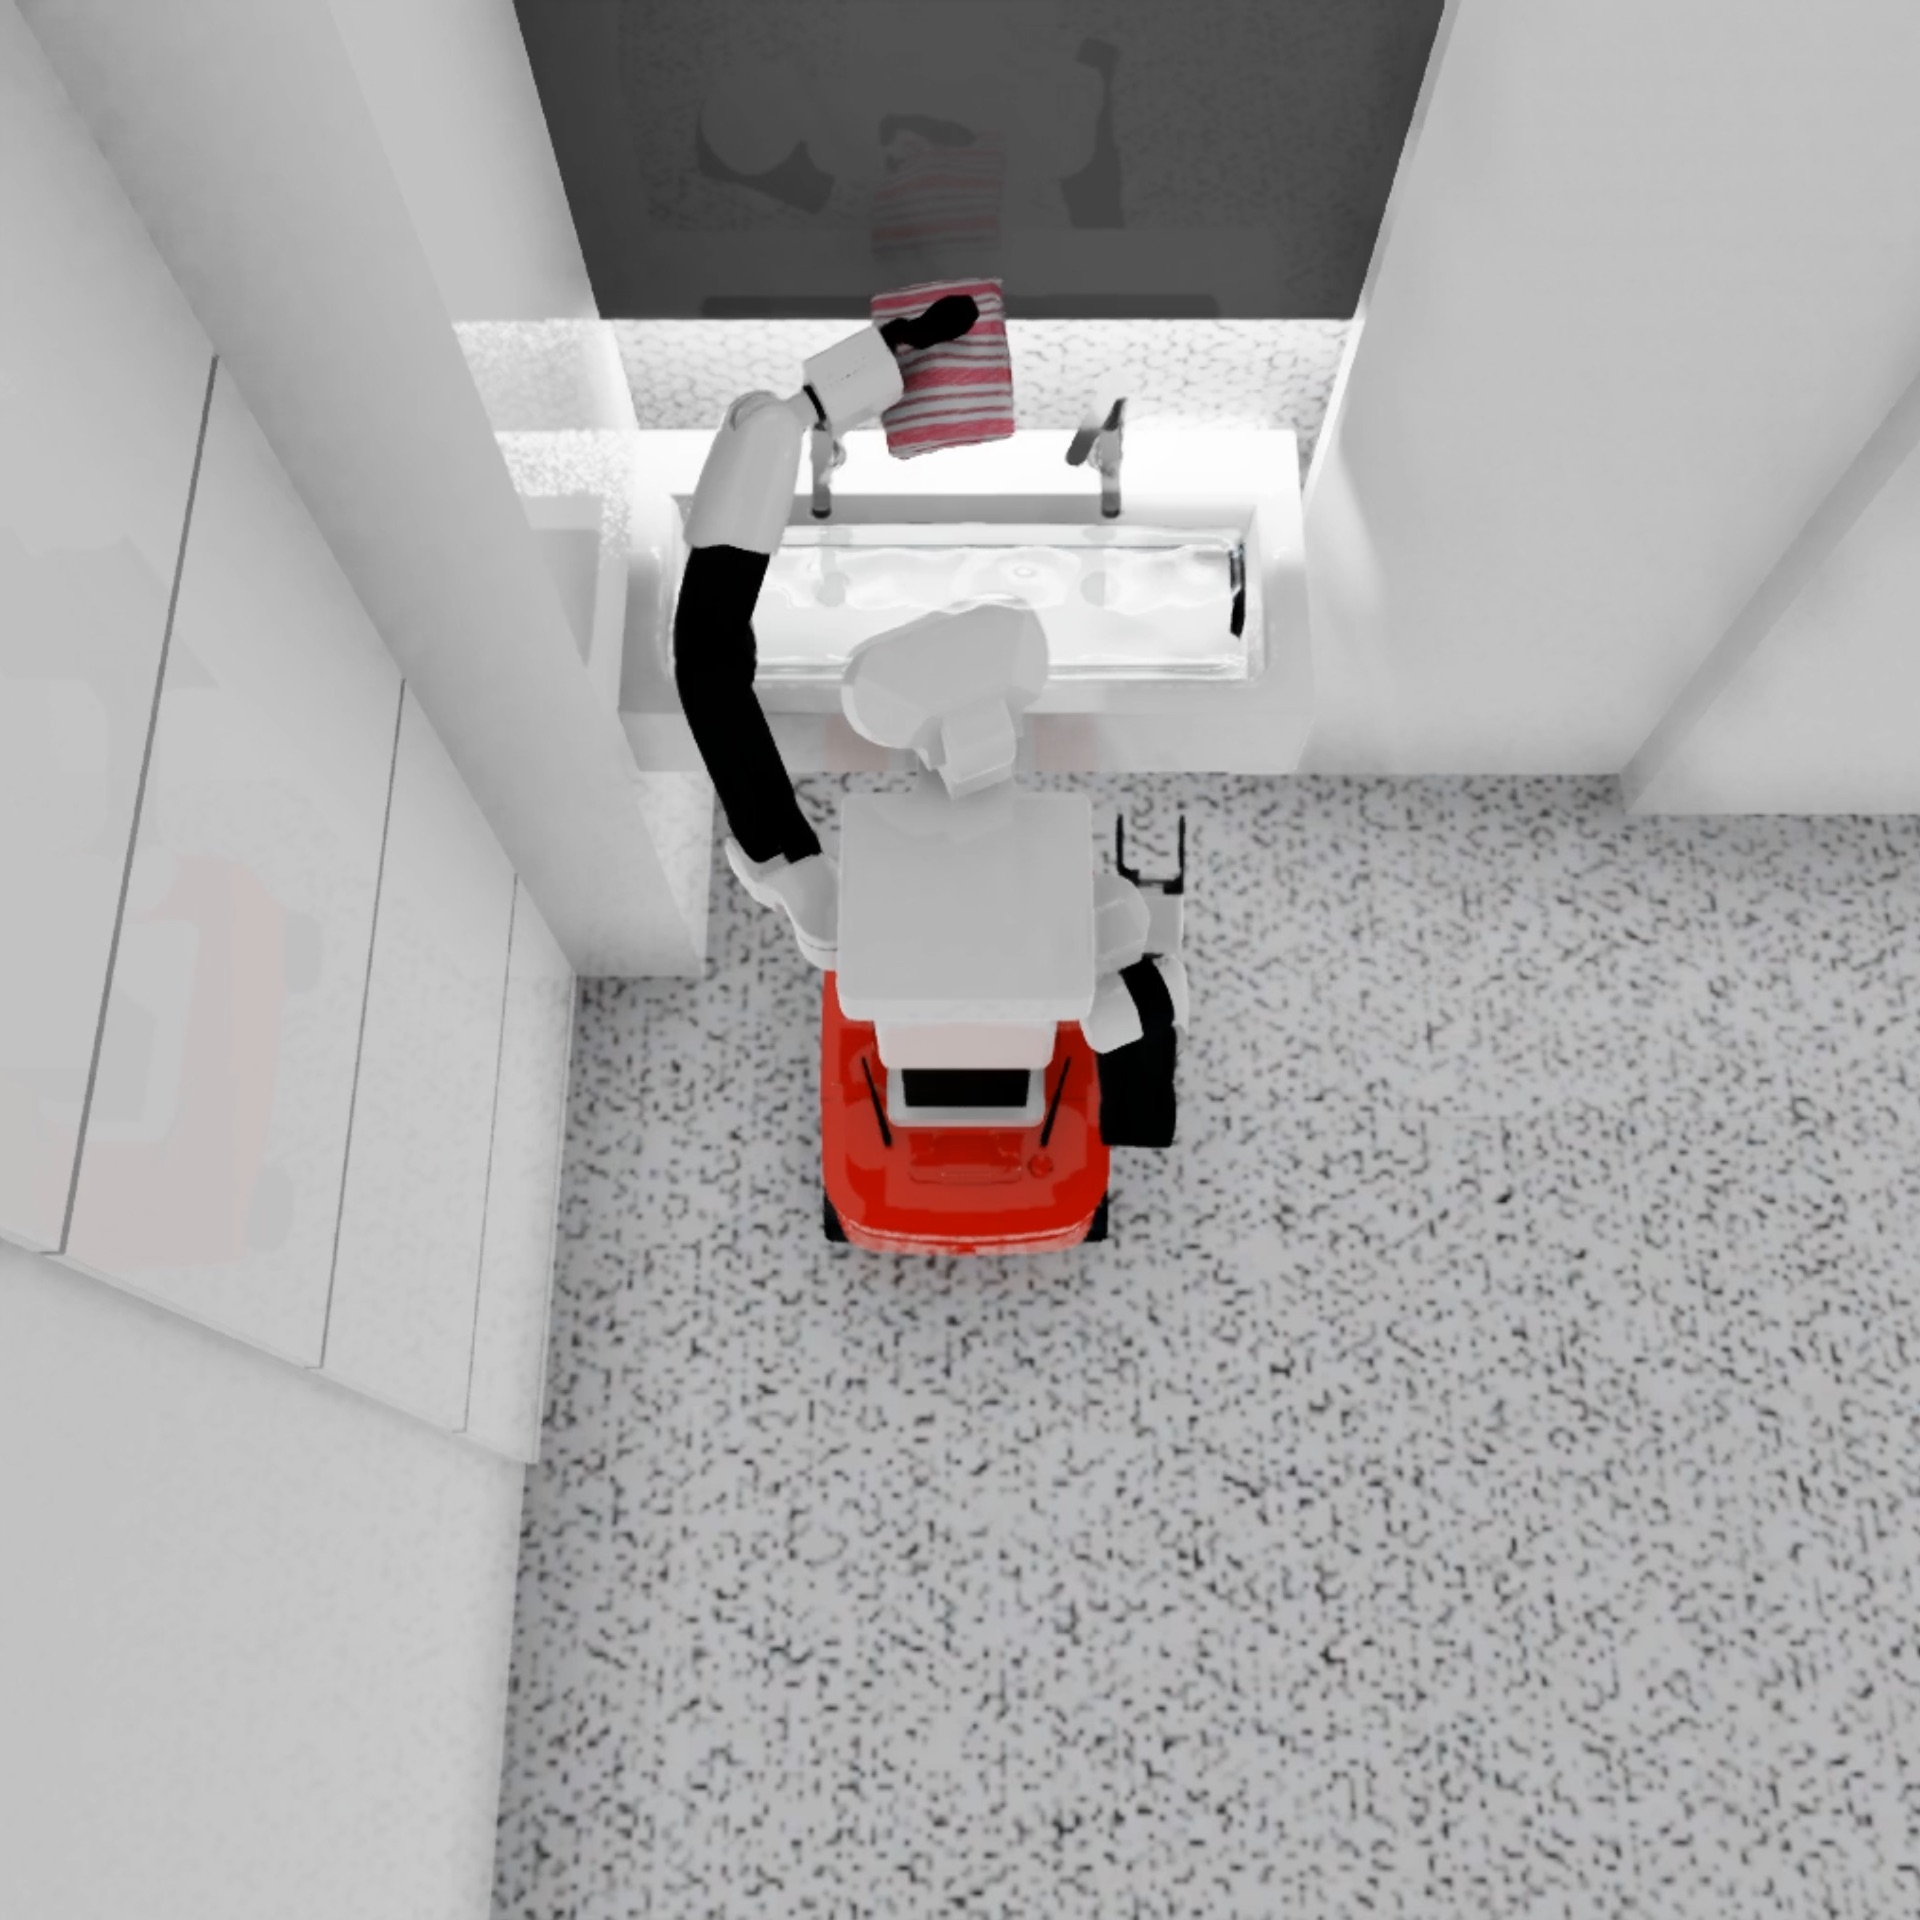
\includegraphics[trim=0 200 0 200,clip,width=0.33\linewidth]{figures/baseline_appendix/dip_1}%
\hfill%
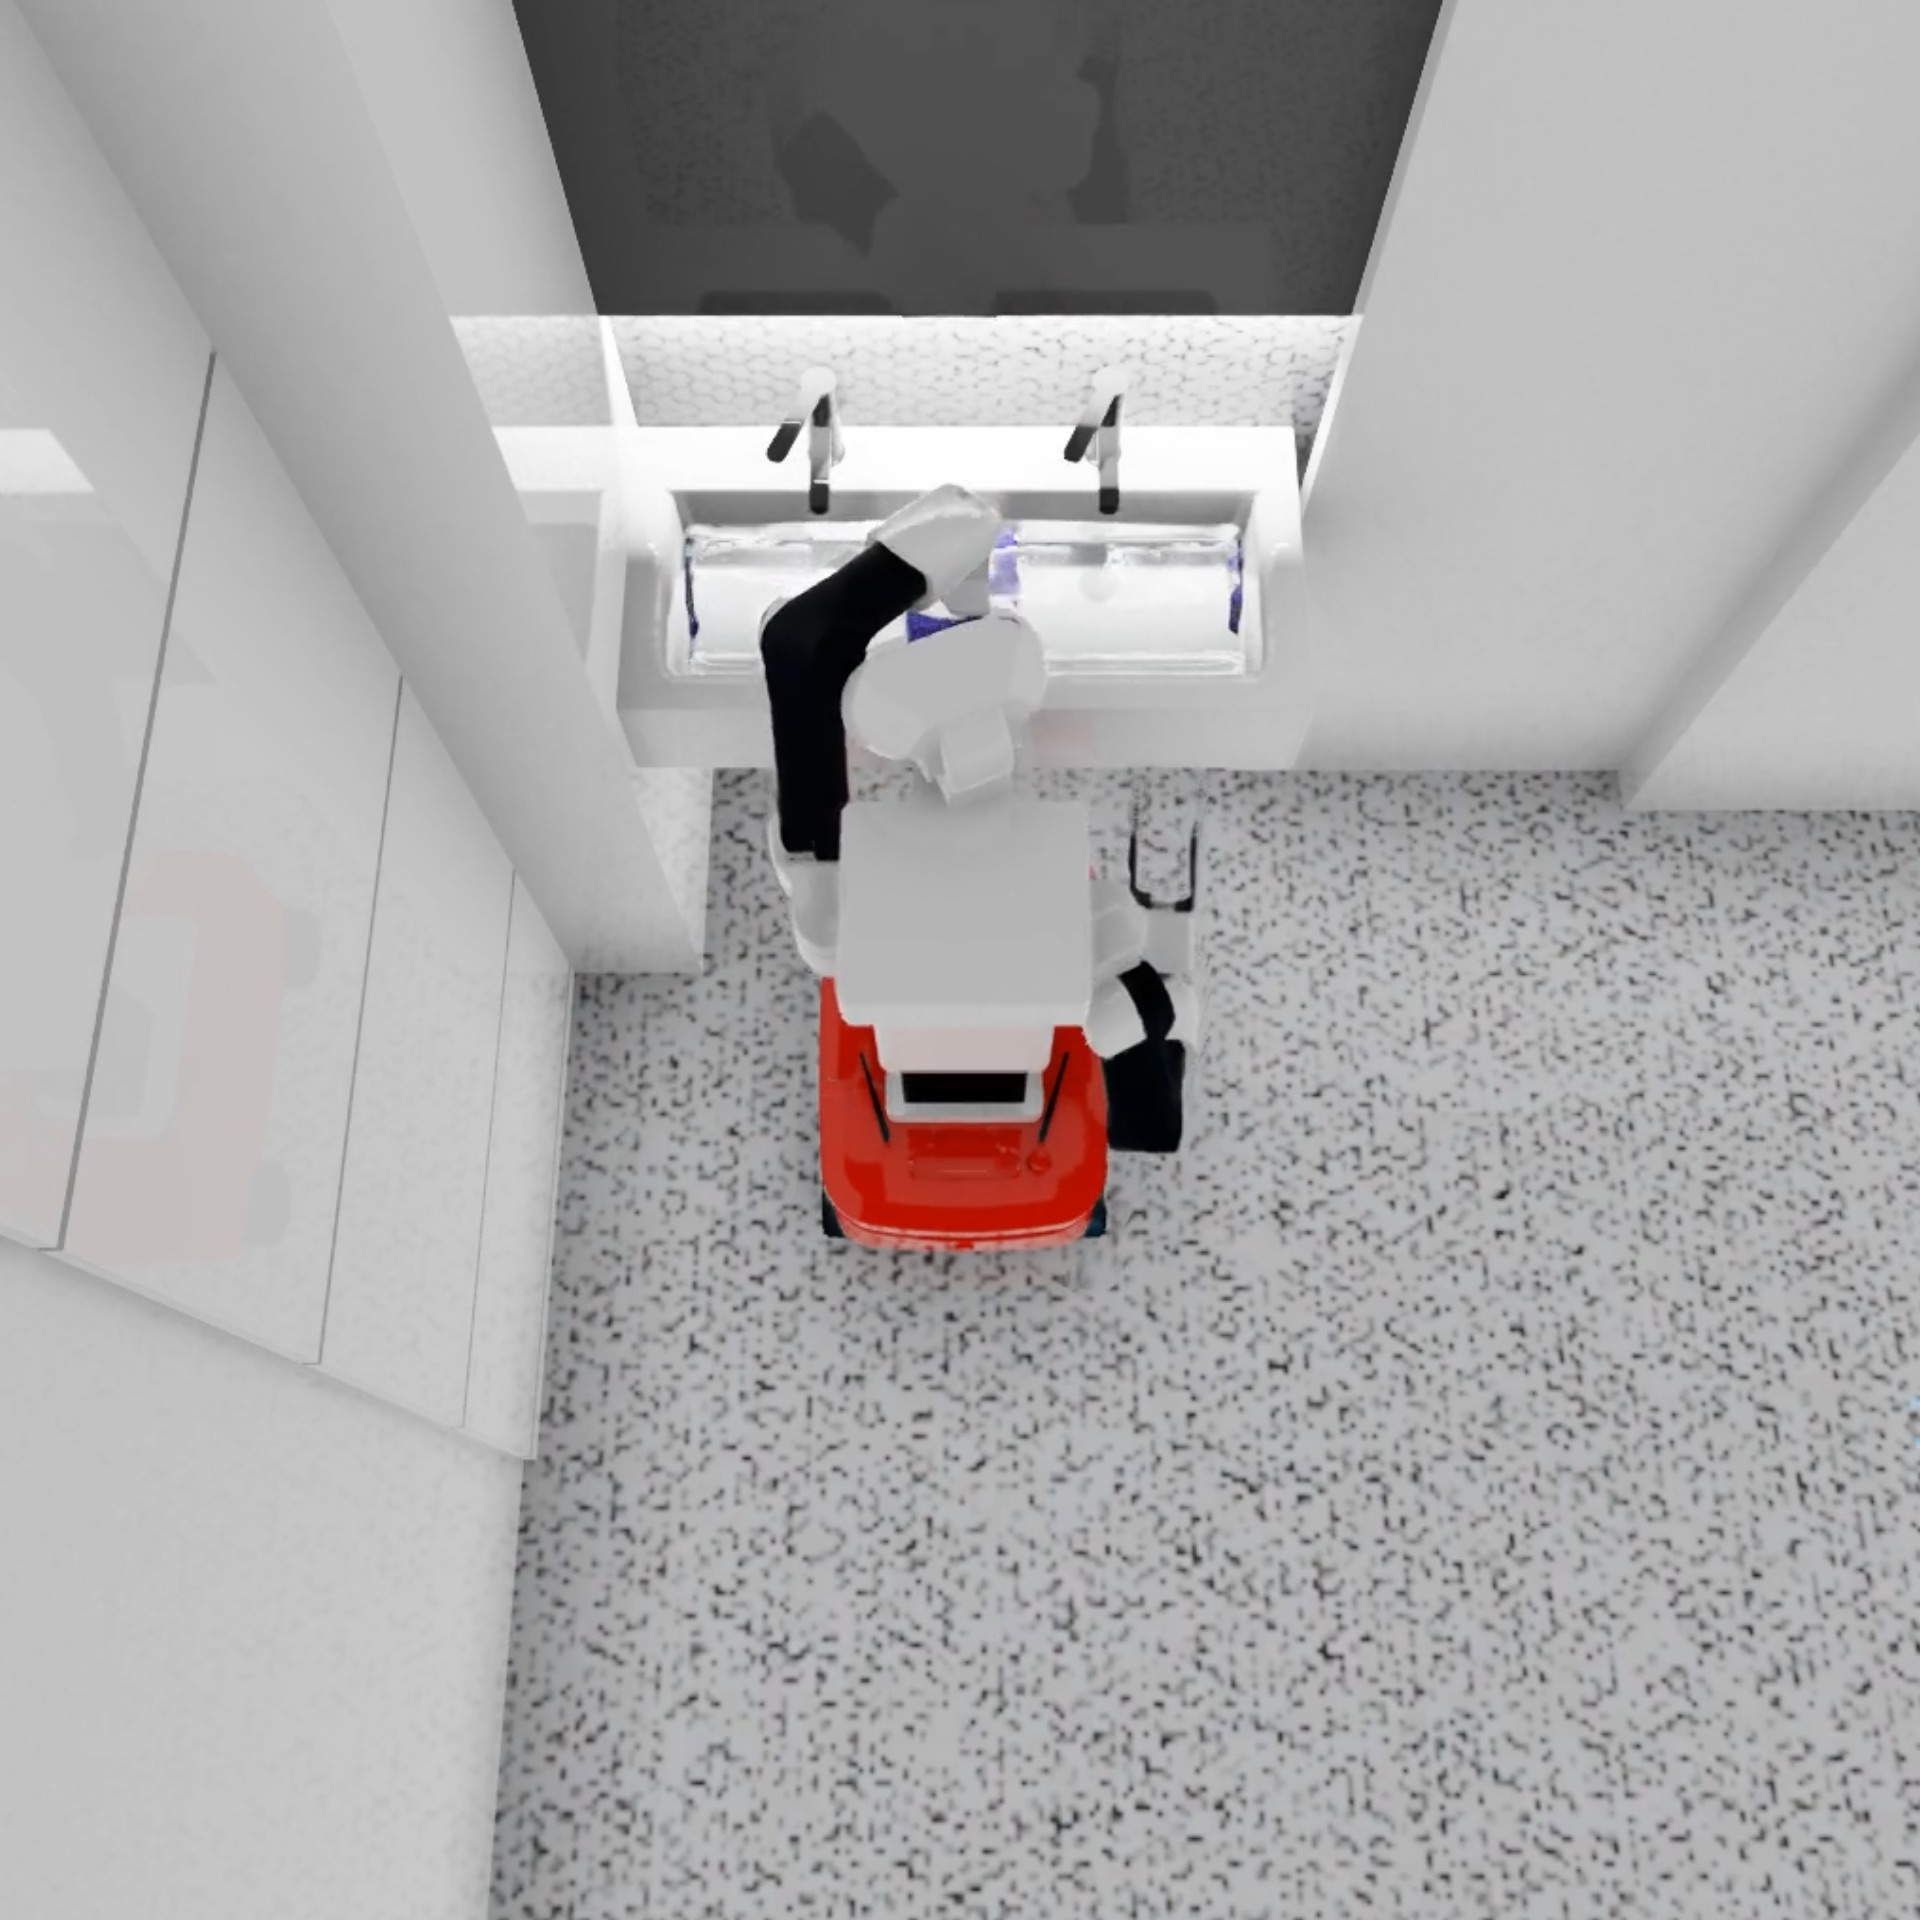
\includegraphics[trim=0 200 0 200,clip,width=0.33\linewidth]{figures/baseline_appendix/dip_2}%
\hfill%
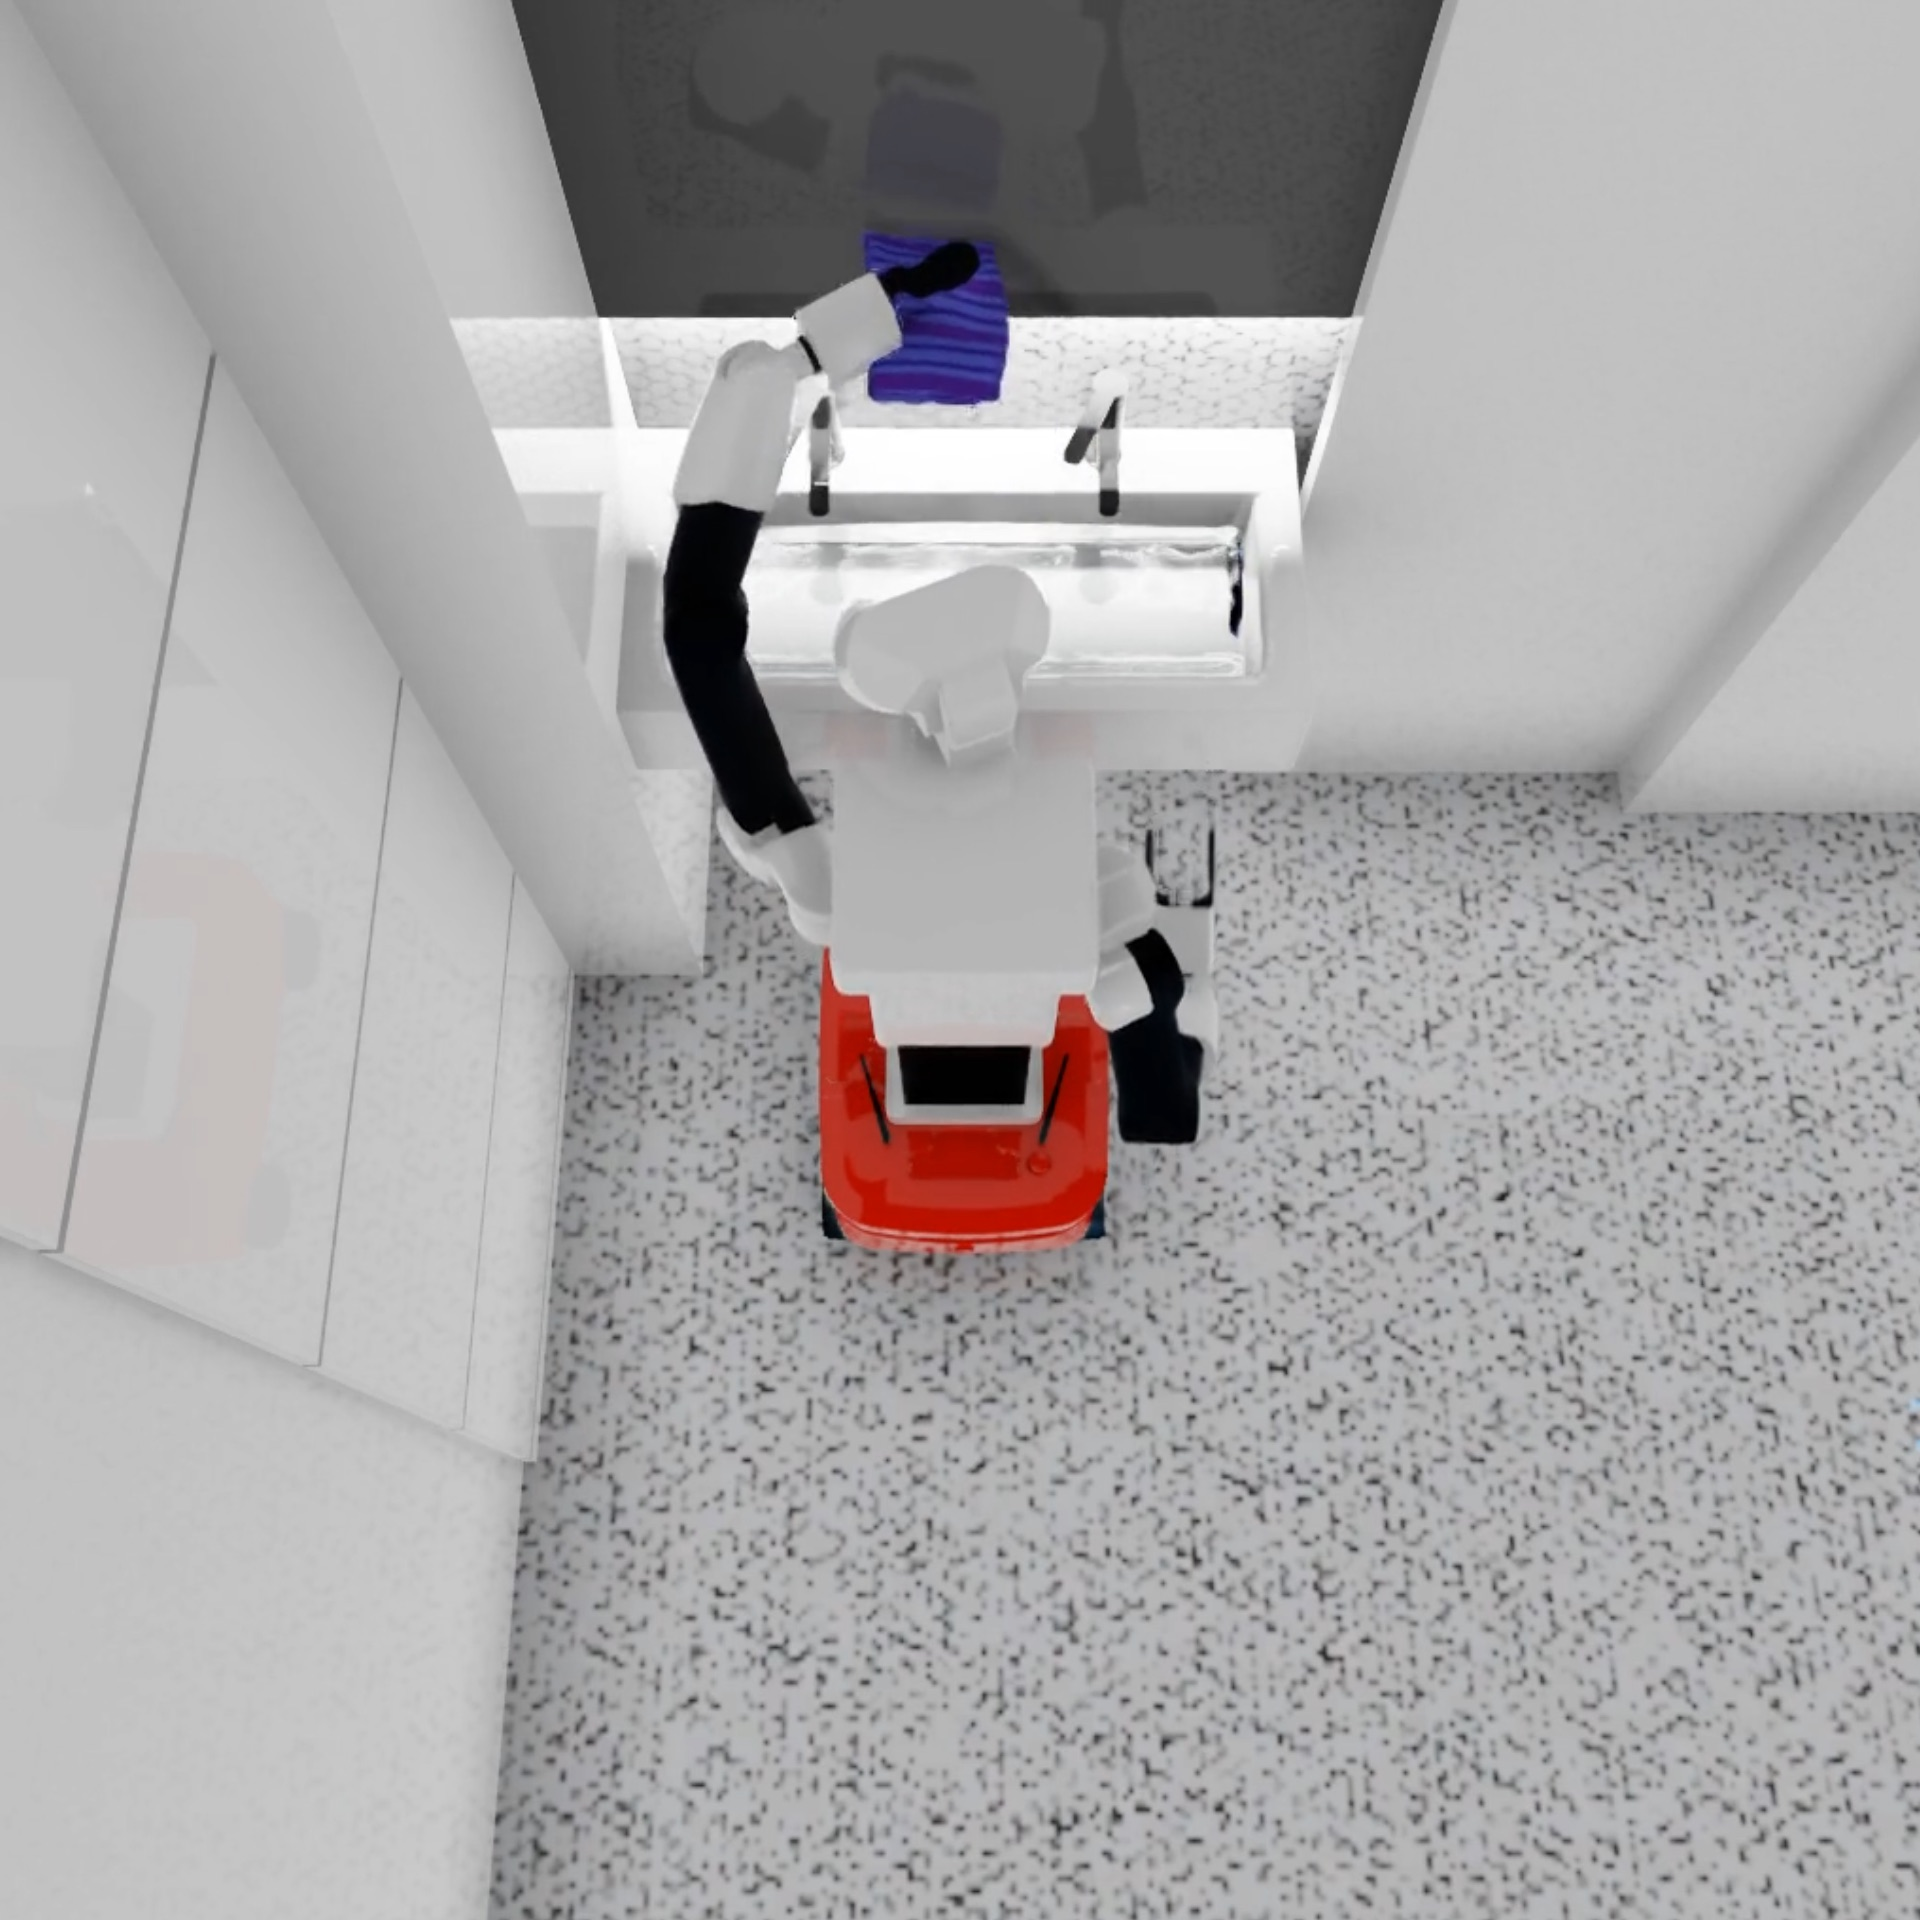
\includegraphics[trim=0 200 0 200,clip,width=0.33\linewidth]{figures/baseline_appendix/dip_3}
}%
\vspace{-5pt}%
\caption{\texttt{dip}}%
\vspace{10pt}%
\end{subfigure}
\begin{subfigure}[t]{0.8\textwidth}{\centering%
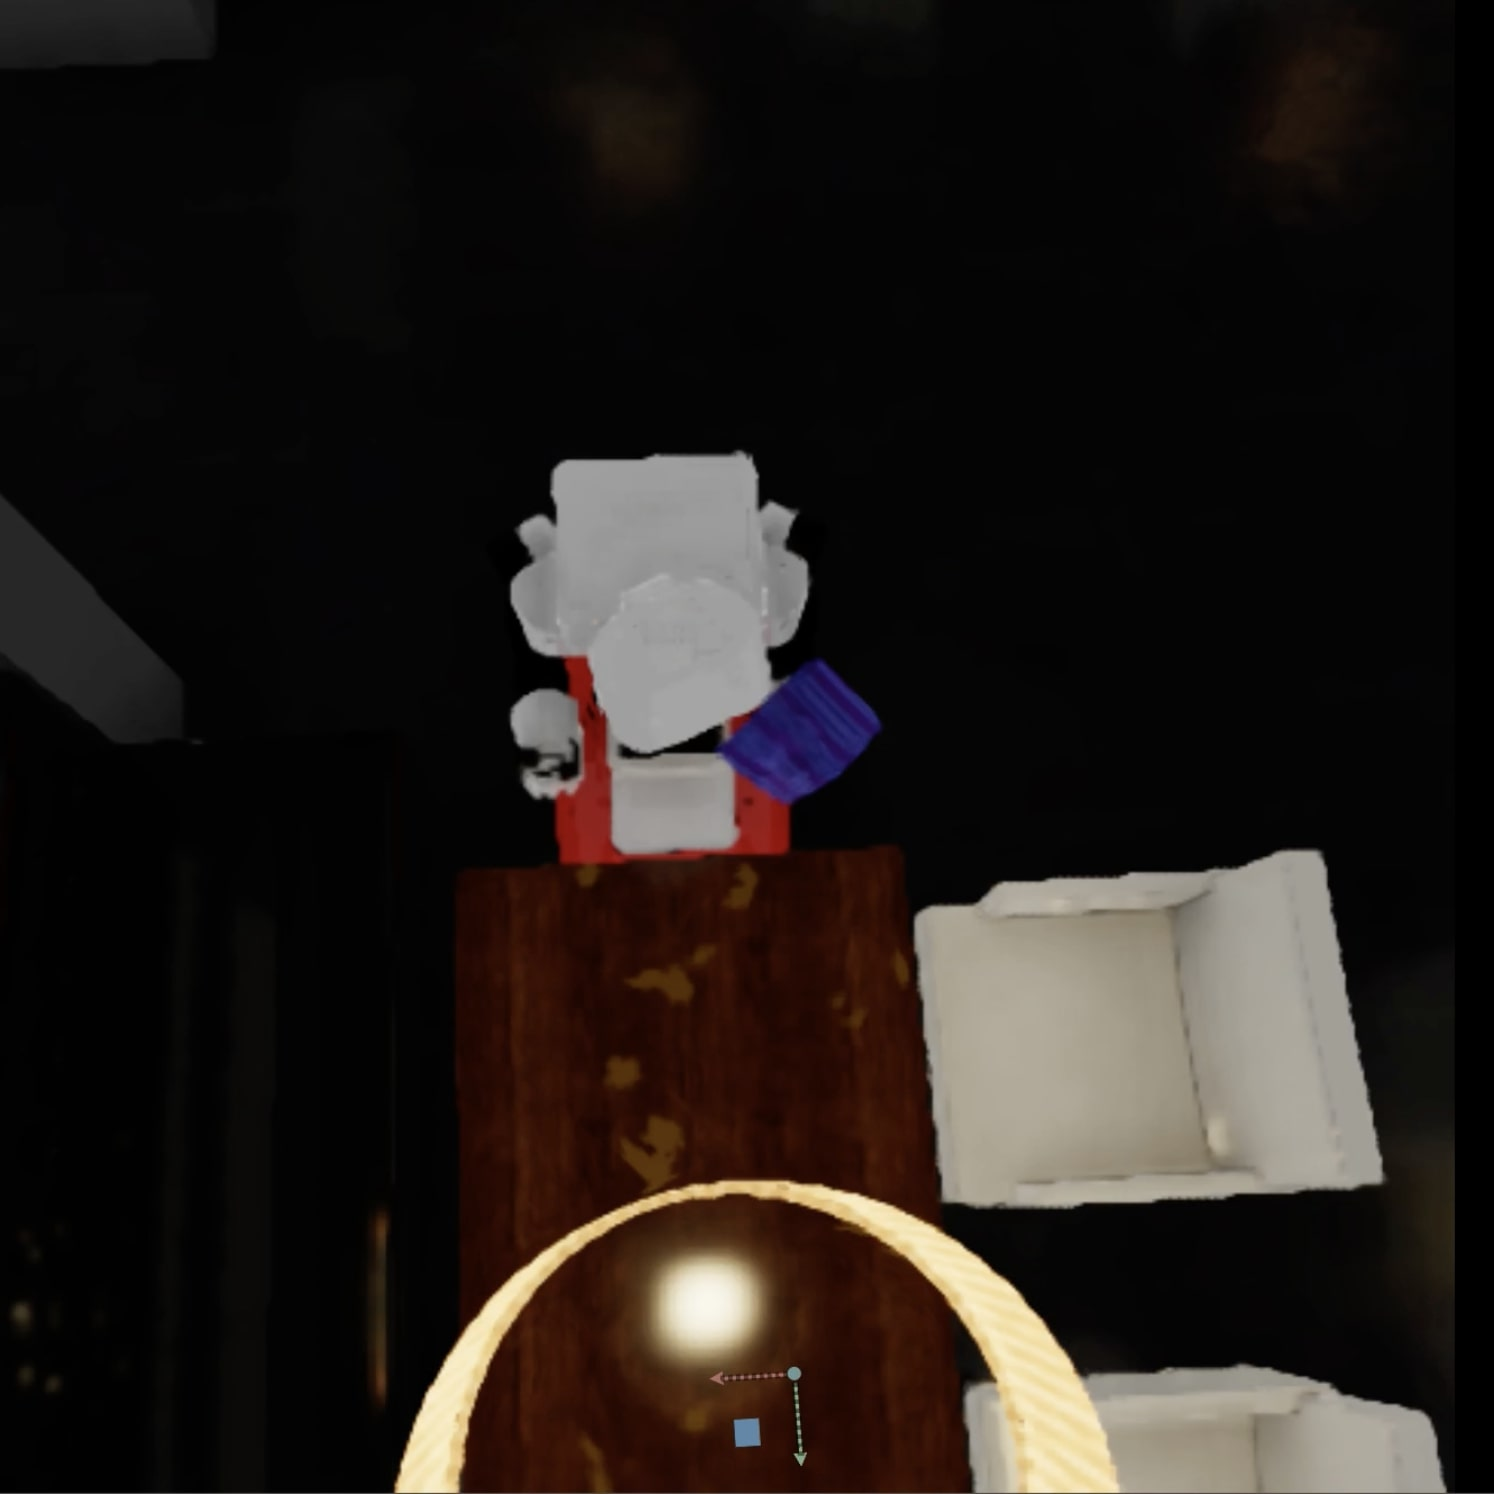
\includegraphics[trim=0 200 0 200,clip,width=0.33\linewidth]{figures/baseline_appendix/wipe_1}%
\hfill%
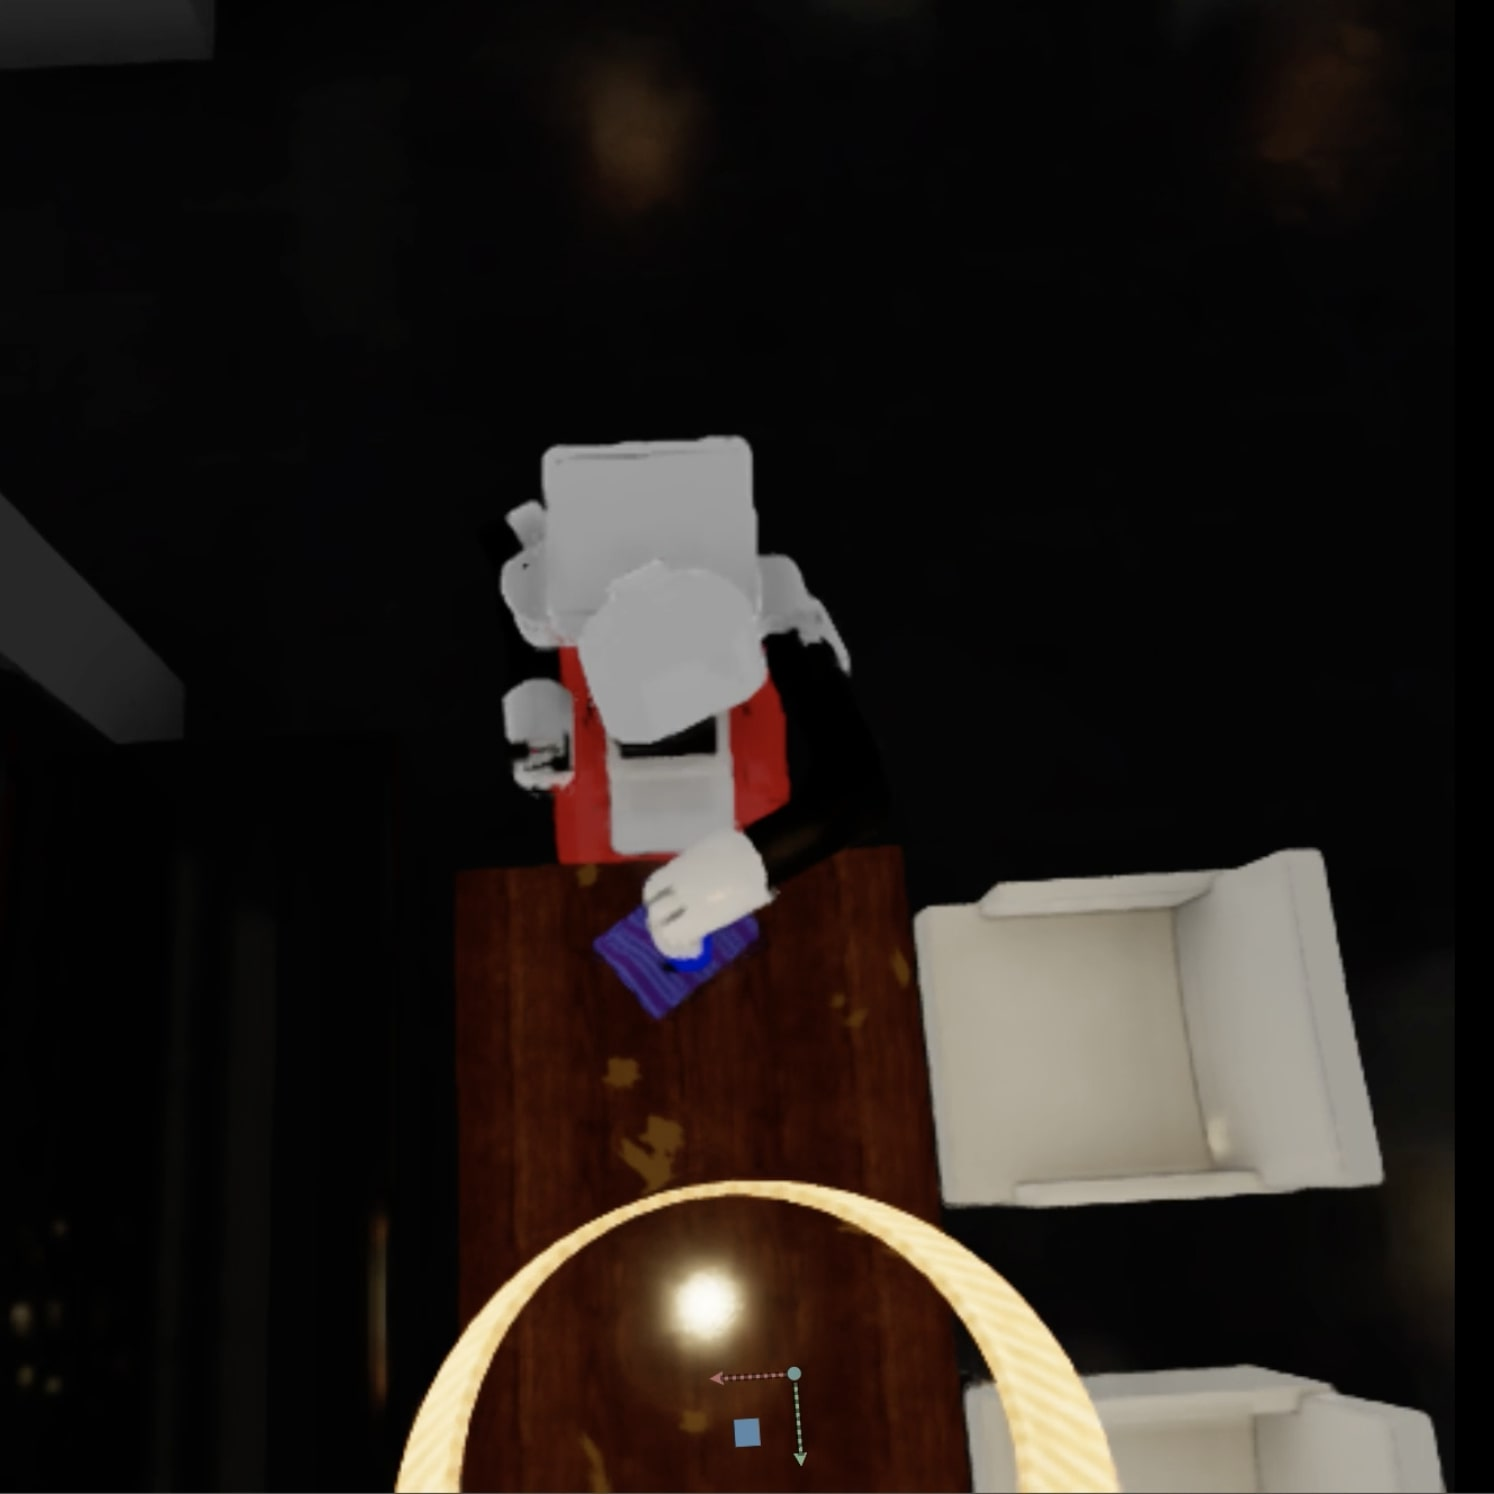
\includegraphics[trim=0 200 0 200,clip,width=0.33\linewidth]{figures/baseline_appendix/wipe_2}%
\hfill%
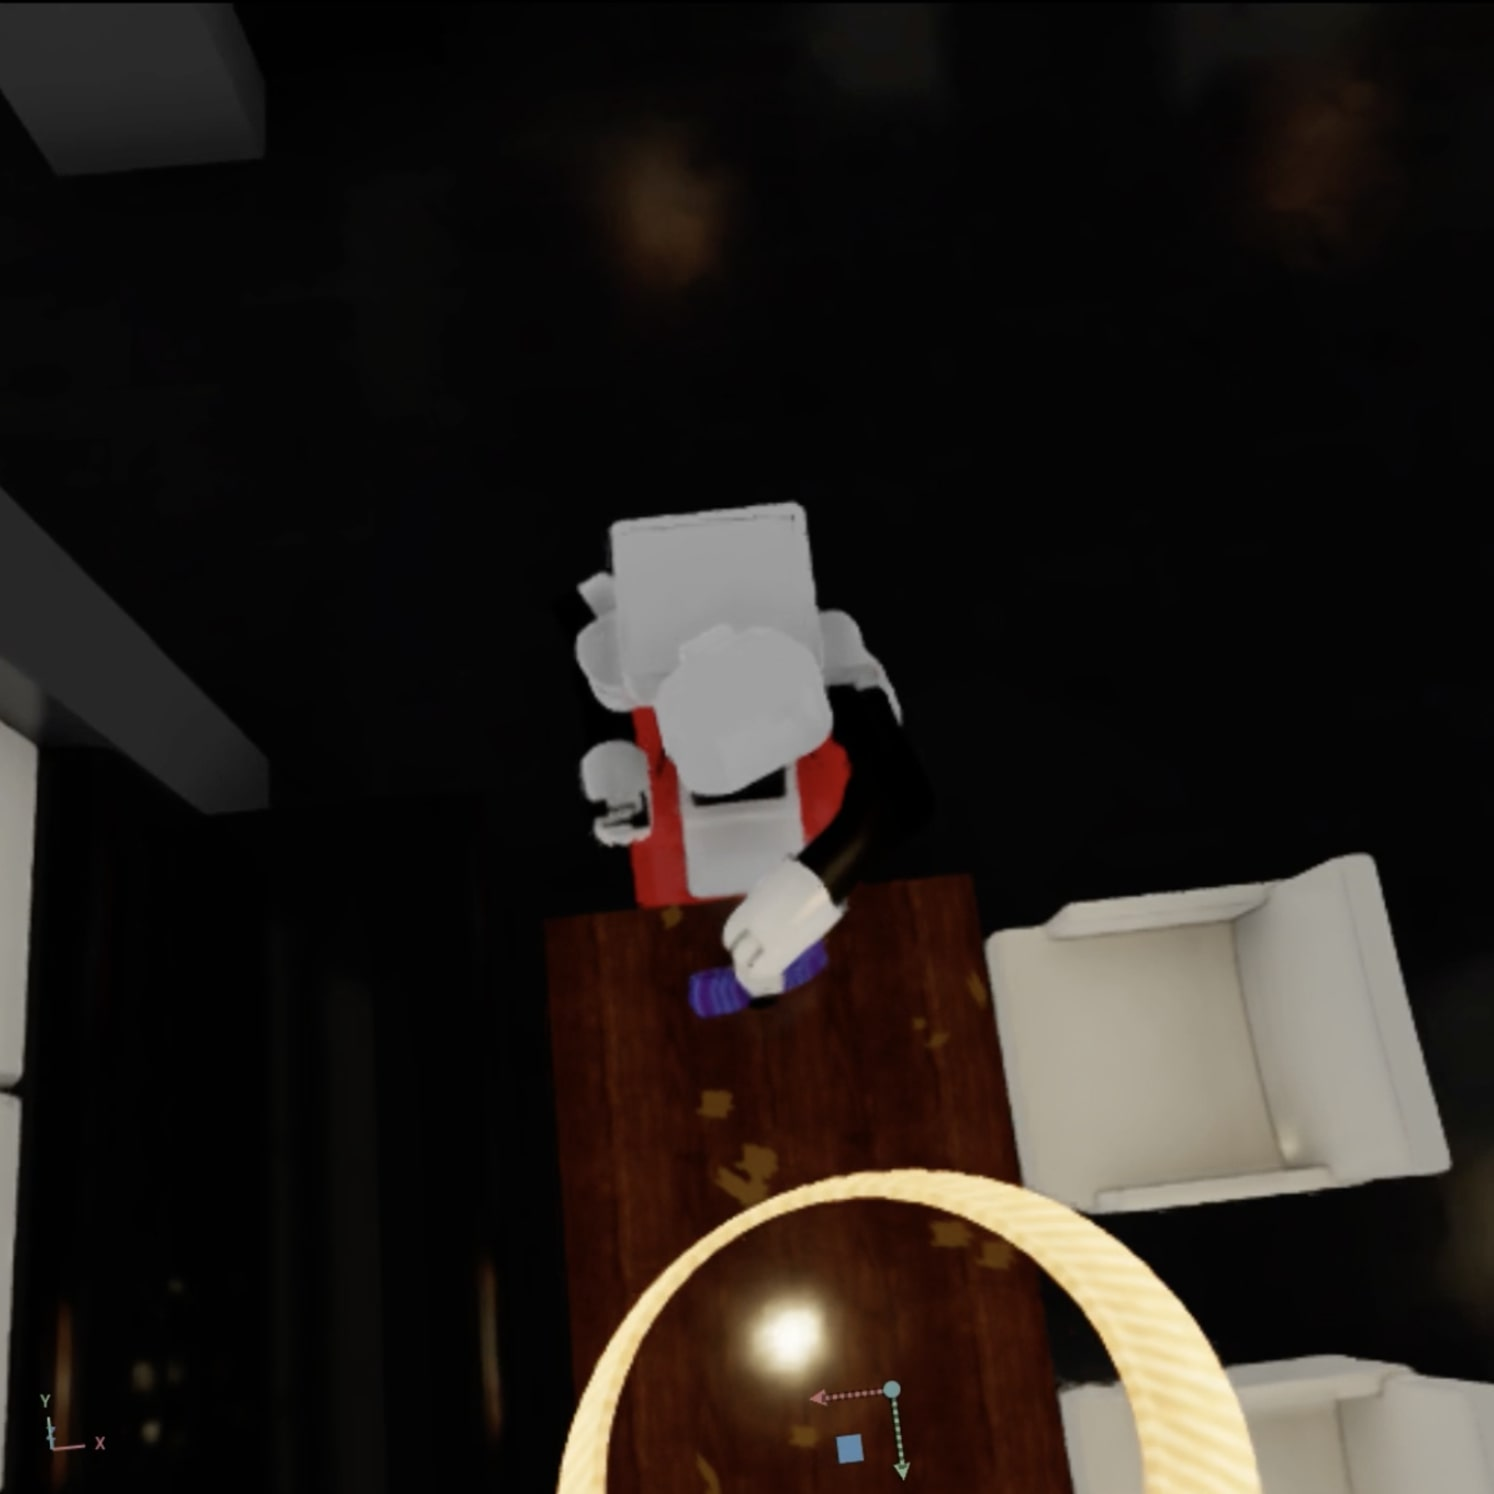
\includegraphics[trim=0 200 0 200,clip,width=0.33\linewidth]{figures/baseline_appendix/wipe_3}
}%
\vspace{-5pt}%
\caption{\texttt{wipe}}%
\vspace{10pt}%
\end{subfigure}
\caption{Overview of all the high-level action primitives with the pre-conditions (left), post-conditions (right), and intermediate states (middle) during execution.
% \roberto{consider taking the images of wipe with more lights, it is hard to see. and the robot is gone in the last image}
}
\label{fig:appendix_high_level_planner}
\end{figure}


\subsection{Additional Metrics: success score Q}
The success score Q \cite{srivastava2021behavior} for each task is reported in Table~\ref{tab:baseline_q_score}. We observe the same trend in Q as in the success rate. This is another indication of the effectiveness of our approach.
\begin{table}[h!]
    \centering
    \resizebox{\textwidth}{!}{\begin{tabular}{l|cc|ccc}
    \toprule
    \multicolumn{1}{c|}{\multirow{2}{*}{Method}} & \multicolumn{2}{c|}{Policy Features} & \multicolumn{3}{c}{Success score Q} \\
    \multicolumn{1}{c|}{} & Primitives & History & \texttt{StoreDecoration} & \texttt{CollectTrash} & \texttt{CleanTable} \\ \midrule
    \rlvmc & \textcolor{red}\faTimes & \textcolor{red}\faTimes & $0.0 \pm 0.0$ & $0.0 \pm 0.0$ & $0.0 \pm 0.0$ \\
    \rlprim & \textcolor{indiagreen}\faCheck & \textcolor{red}\faTimes & $0.50 \pm 0.05$ & $0.49 \pm 0.04$ & $0.77 \pm 0.08$ \\
    \rlprimhist & \textcolor{indiagreen}\faCheck & \textcolor{indiagreen}\faCheck & $0.59 \pm 0.03$ & $0.68 \pm 0.02$  & $0.88 \pm 0.02$ \\ \bottomrule
    \end{tabular}
    }
    \caption{Performance of three baseline methods, in terms of the success score Q.}
    \label{tab:baseline_q_score}
\end{table}


\begin{figure}
    \centering
    \begin{tabular}{cc}        
        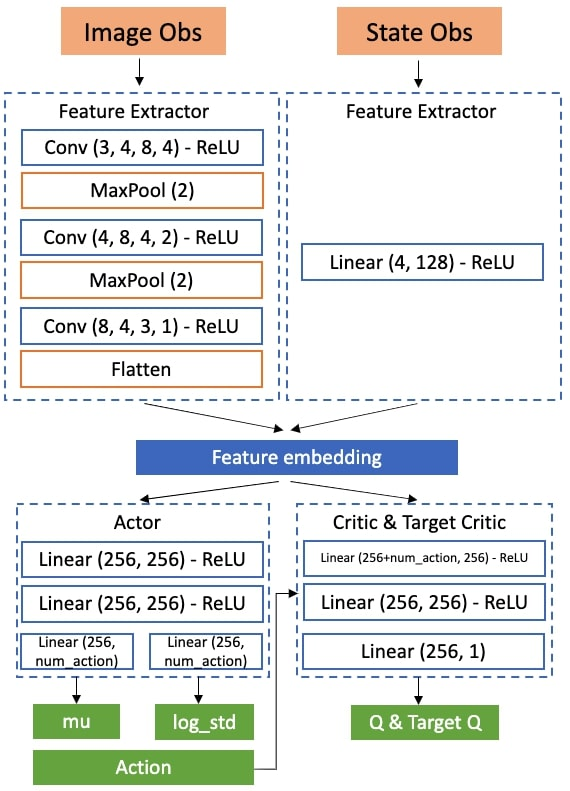
\includegraphics[width=0.45\linewidth]{figures/baseline_appendix/sac} &
        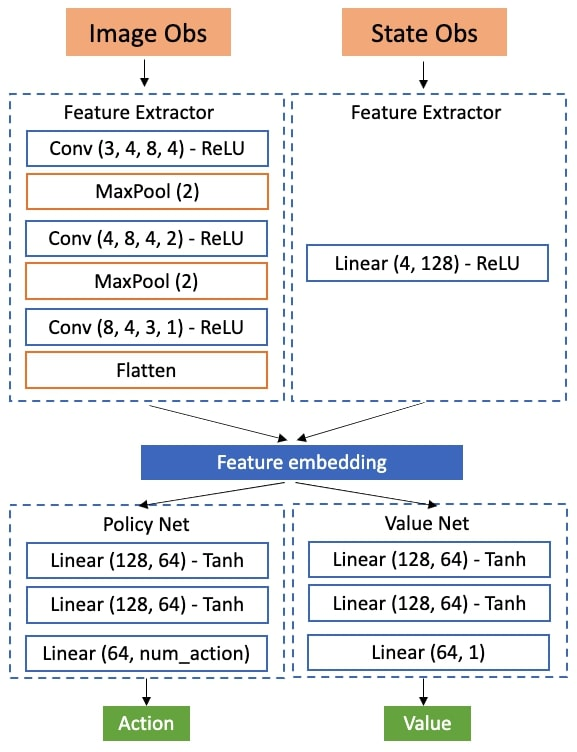
\includegraphics[width=0.45\linewidth]{figures/baseline_appendix/ppo} \\
        a) SAC Architecture & b) PPO Architecture \\
    \end{tabular}
    \caption{%\todo{VMC polict architecture} 
    Policy architecture of SAC (\rlvmc) and PPO (\rlprim and \rlprimhist). The policy maps egocentric visual observations and proprioceptive information into an action that controls the robot base, arm, and gripper. PPO outputs a discrete high-level action primitive while SAC outputs a continuous low-level joint control directly.%\roberto{make jpeg or even better, export the original as vectorgraphics/pdf}
    }
    \label{fig:appendix_ppo_vmc_arch}
\end{figure}



% \begin{figure*}[t]
% \centering
% \begin{minipage}[c]{\linewidth}
% \centering
%     \renewcommand\tabcolsep{0.5pt}
%     \begin{tabular}{ccc}
%         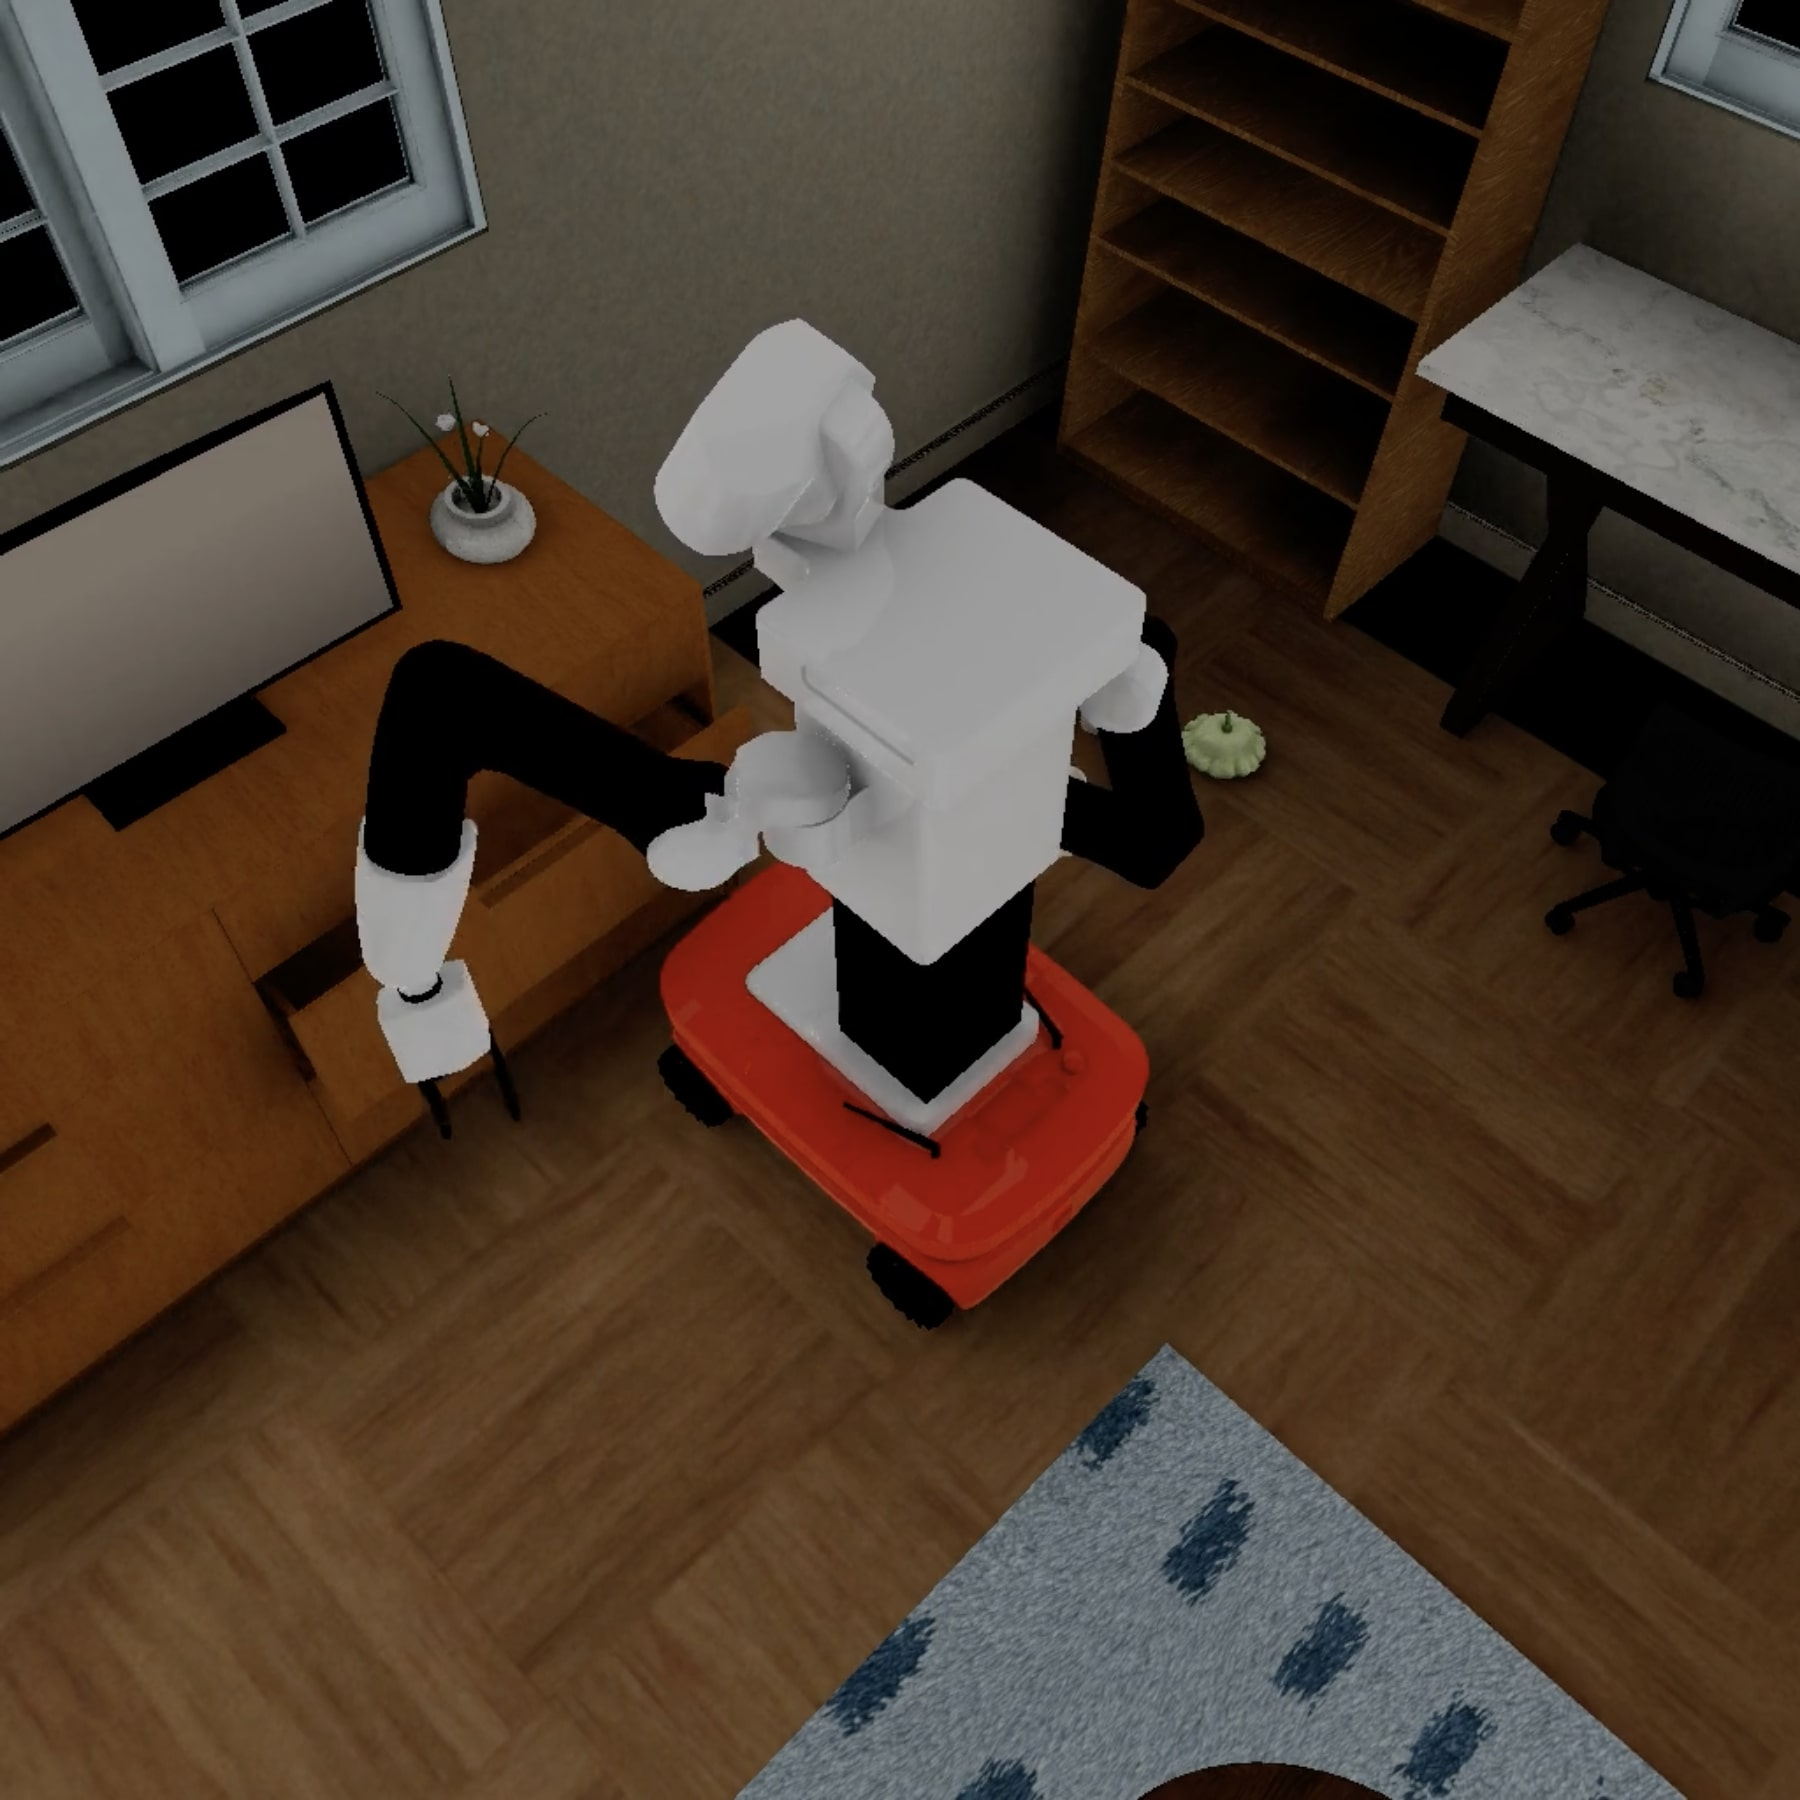
\includegraphics[width=0.3\linewidth]{figures/baseline_appendix/store_decoration_1.png}&
%         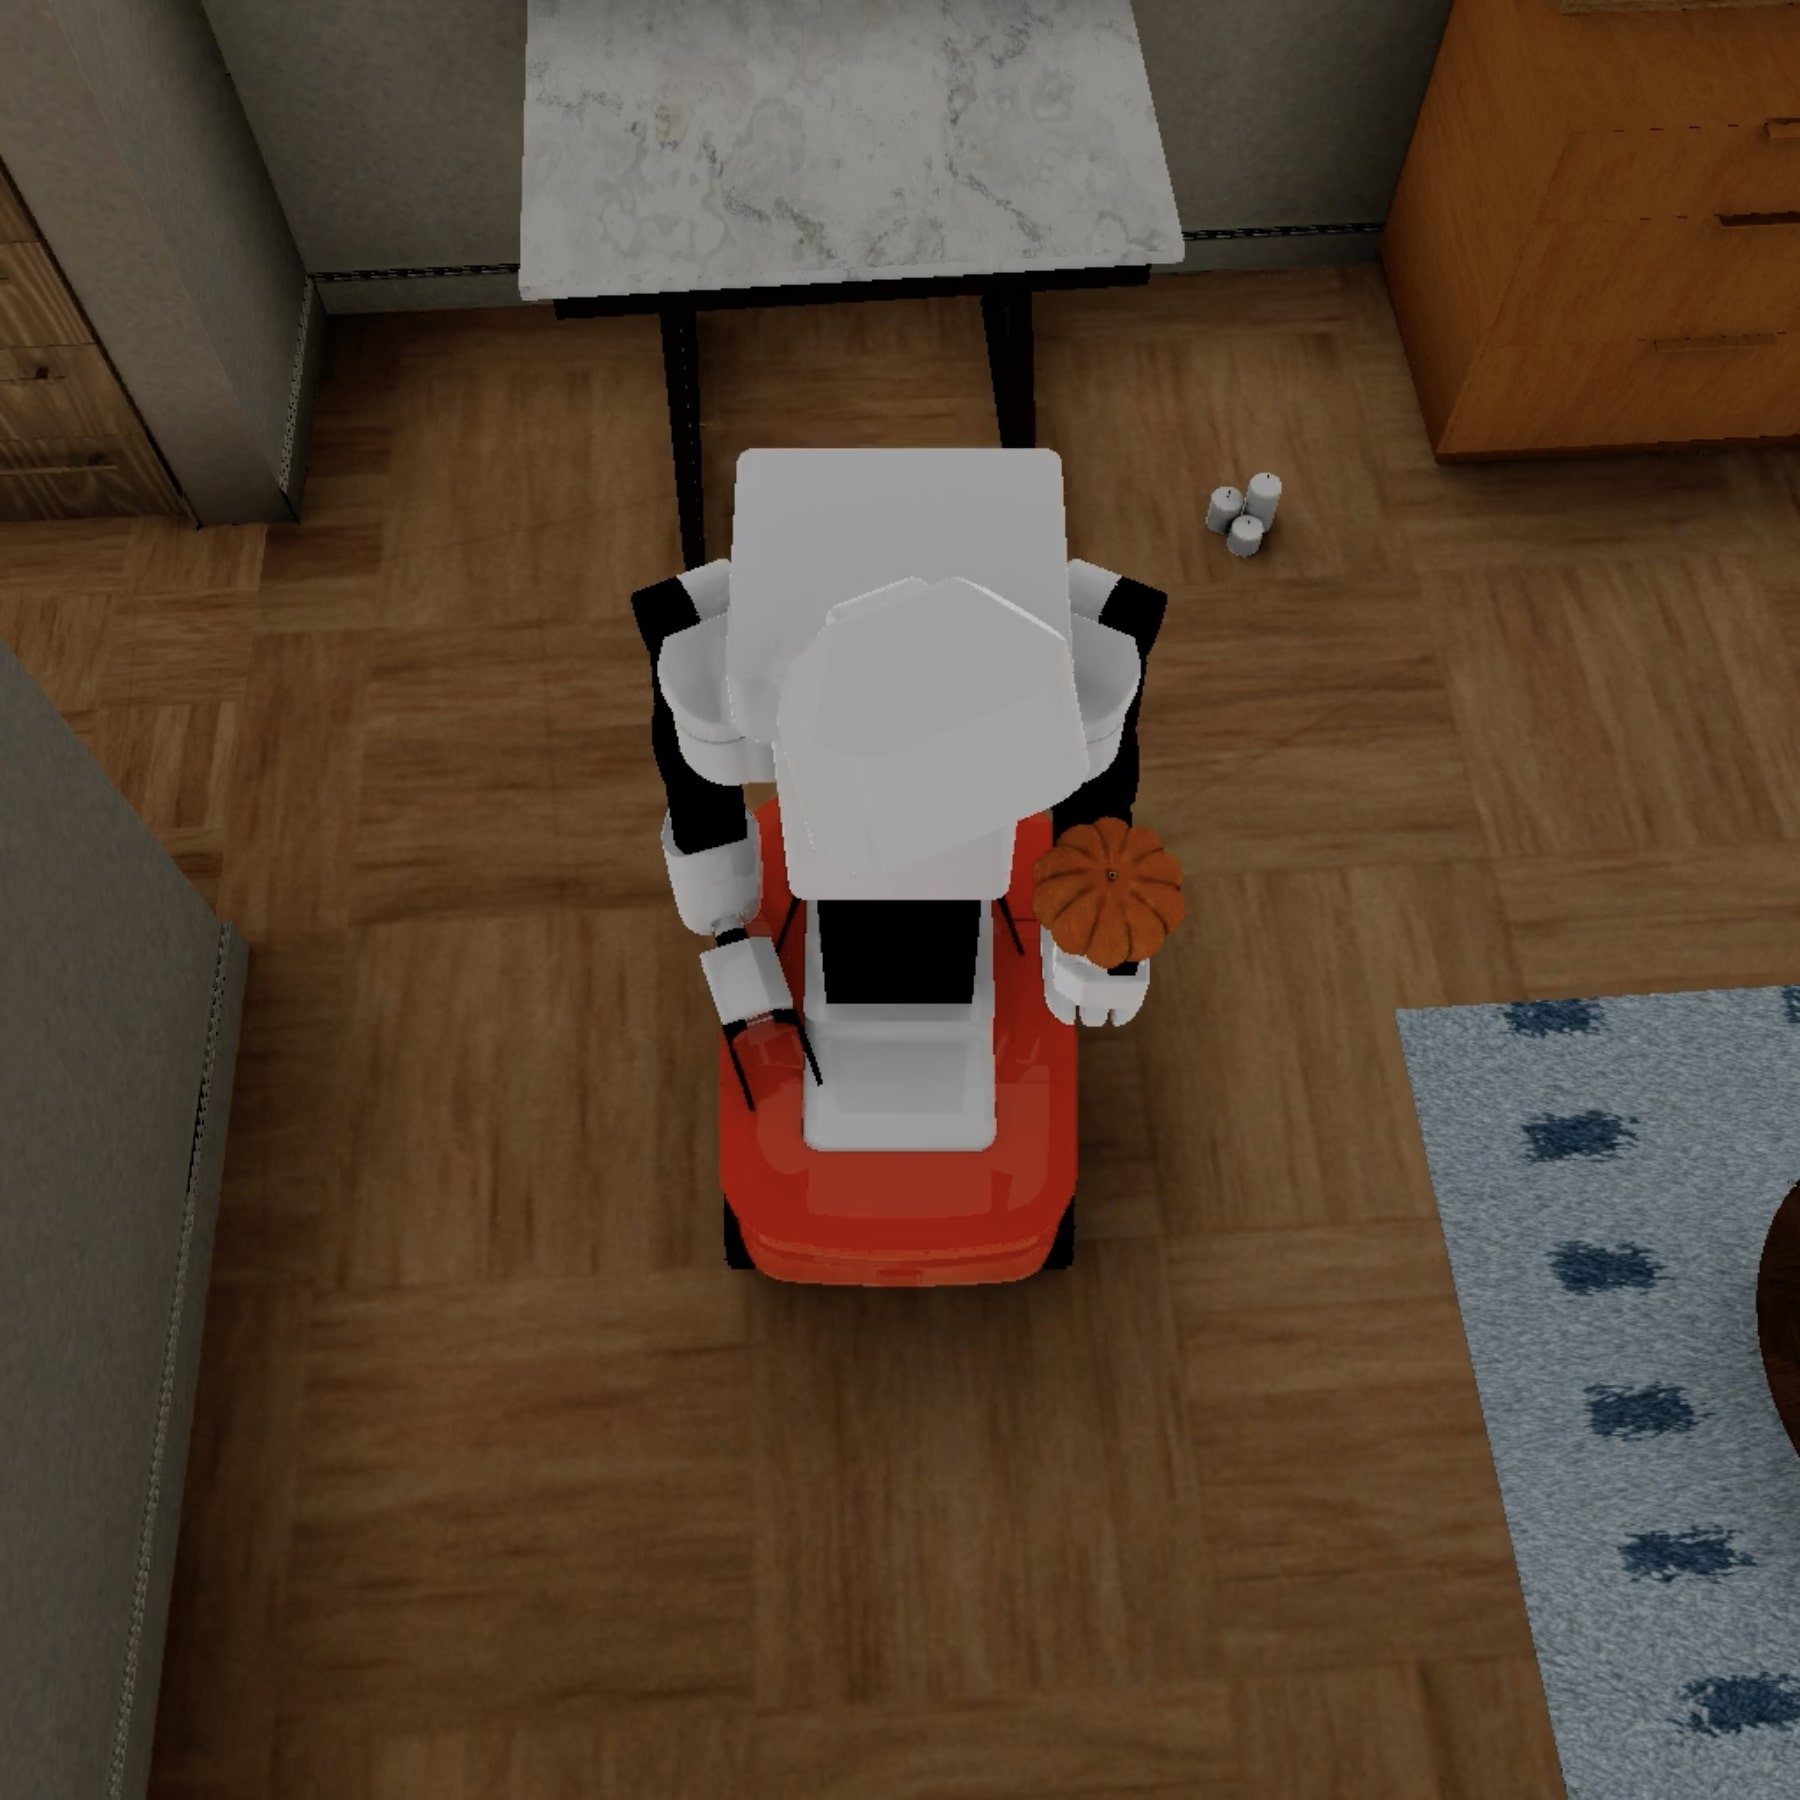
\includegraphics[width=0.3\linewidth]{figures/baseline_appendix/store_decoration_2.png}&
%         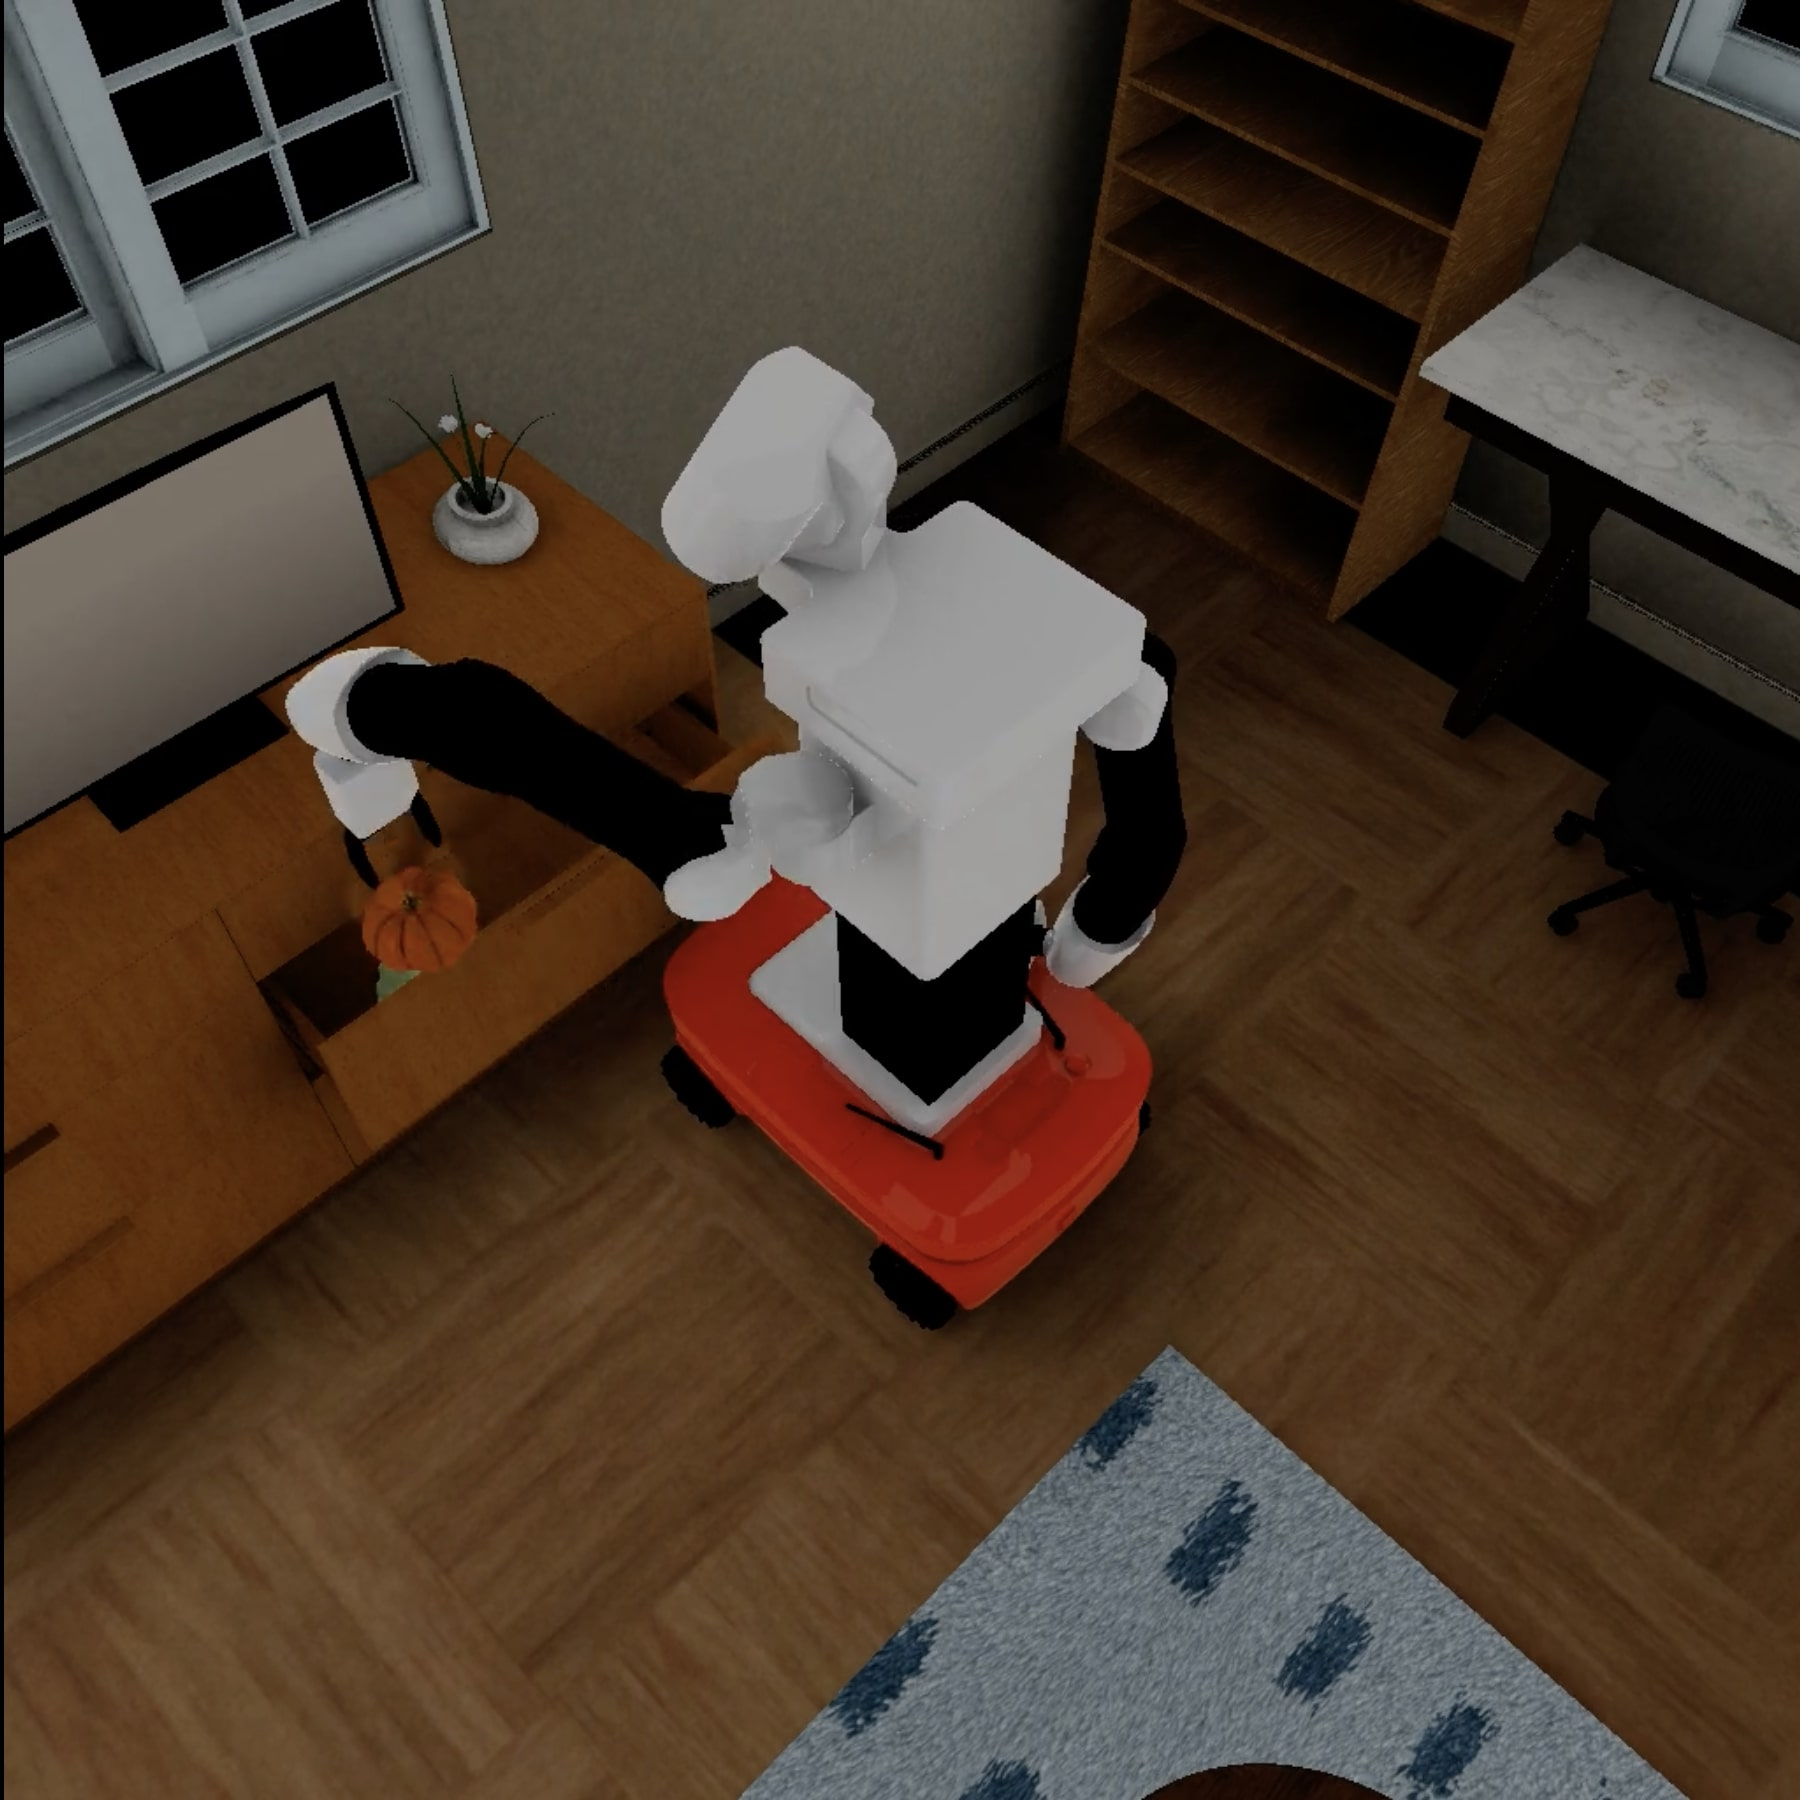
\includegraphics[width=0.3\linewidth]{figures/baseline_appendix/store_decoration_3.png}\\
%         & a) Store Decoration & \\
%         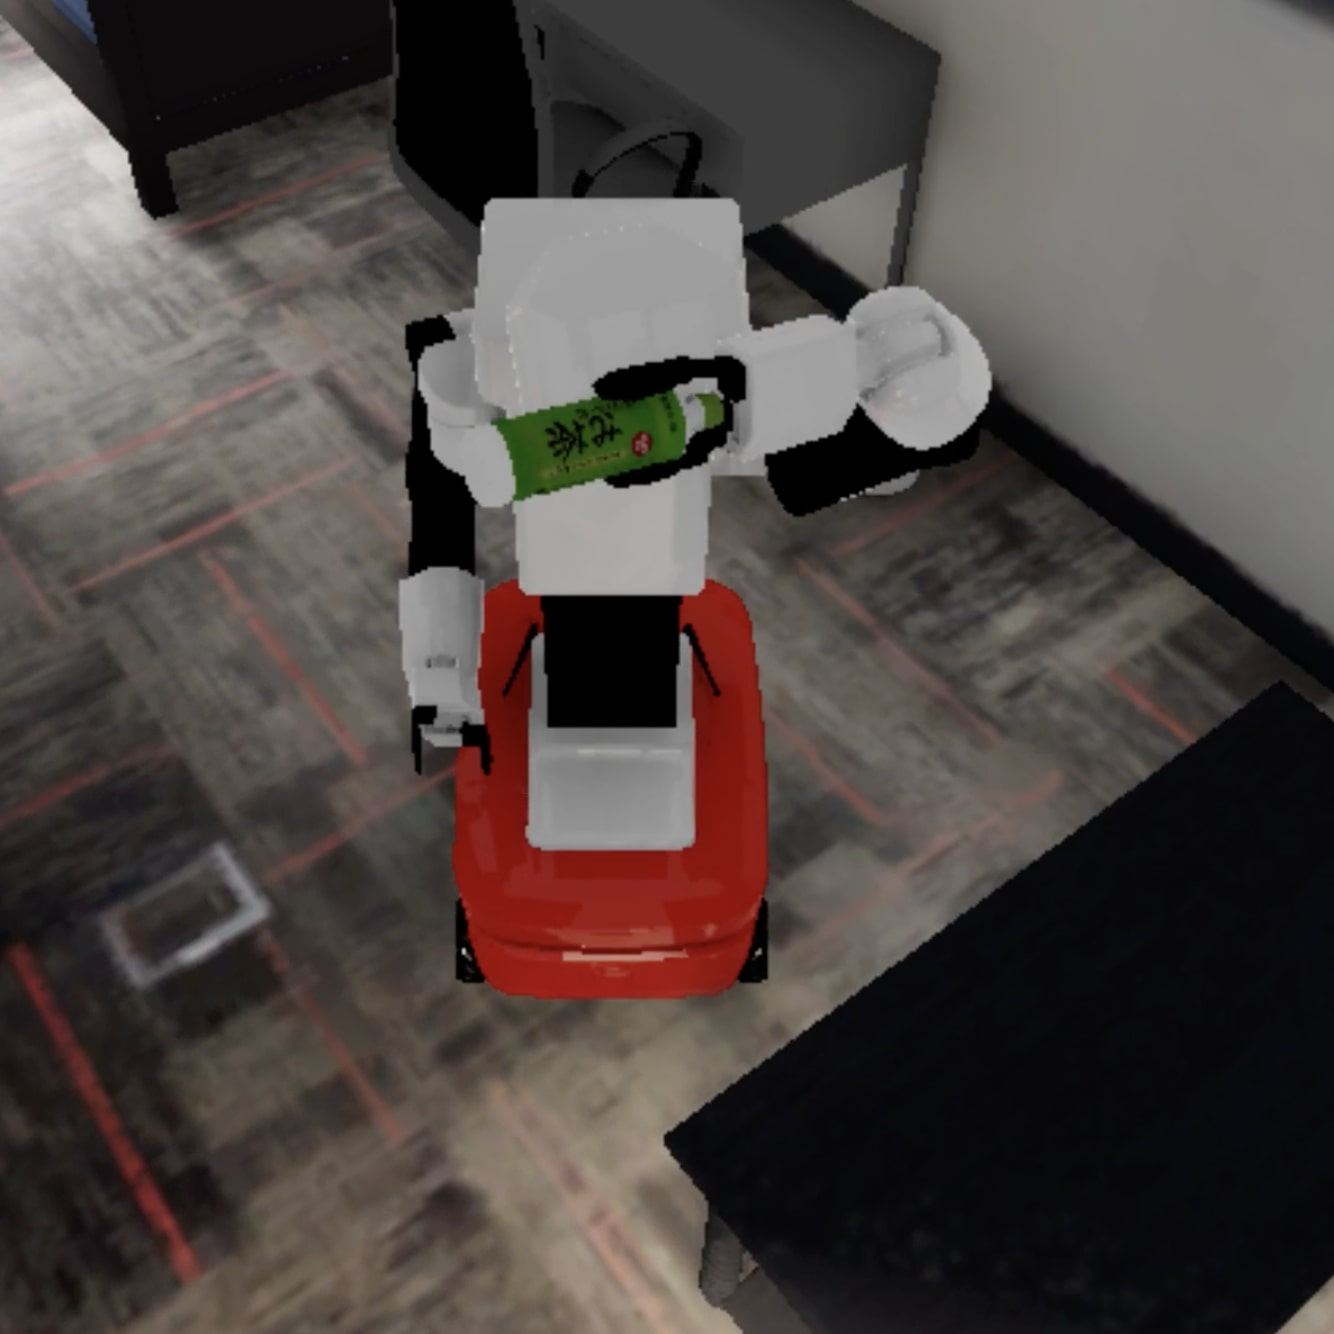
\includegraphics[width=0.3\linewidth]{figures/baseline_appendix/collect_trash_1.png}&
%         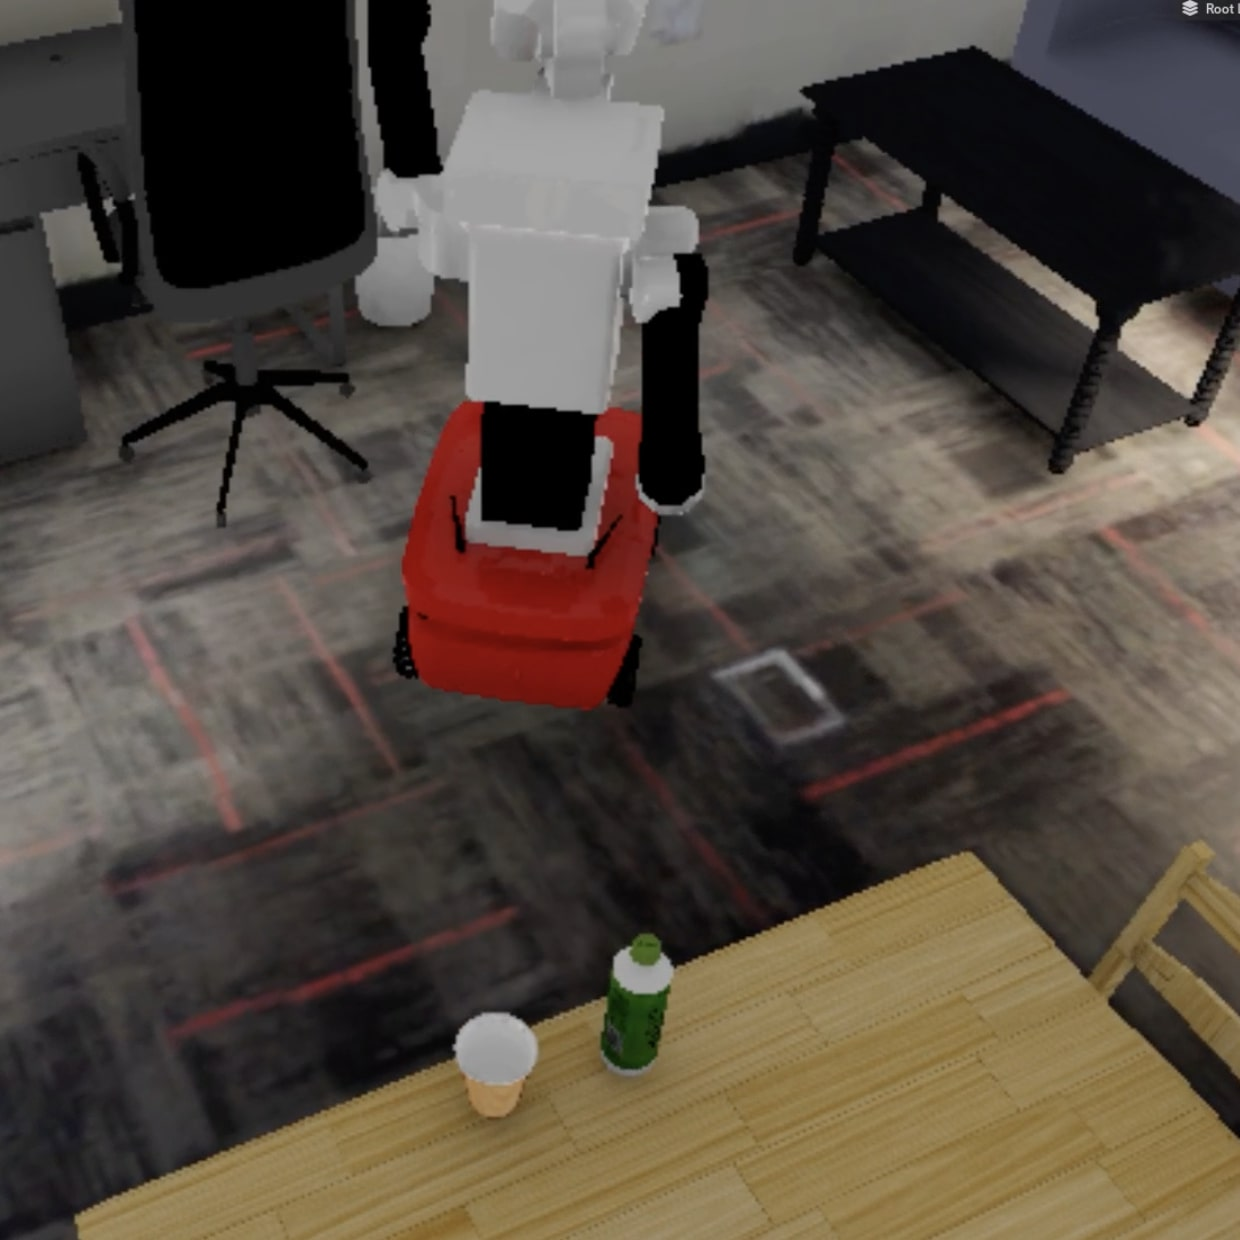
\includegraphics[width=0.3\linewidth]{figures/baseline_appendix/collect_trash_2.png}&
%         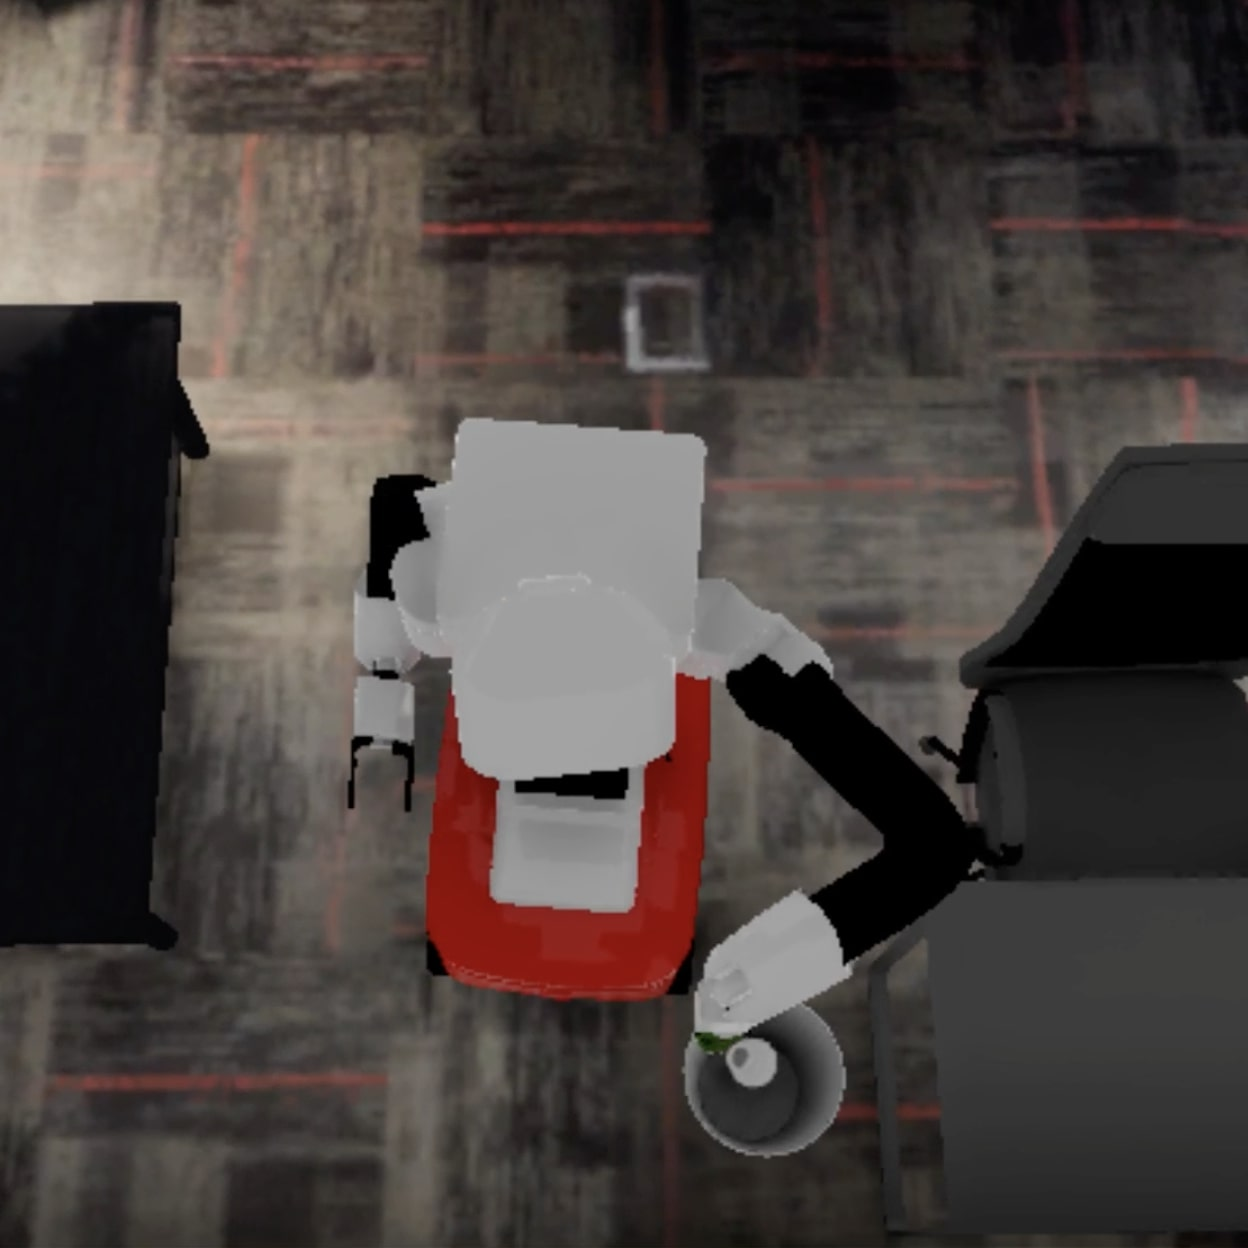
\includegraphics[width=0.3\linewidth]{figures/baseline_appendix/collect_trash_3.png}\\
%         & b) Collect Trash & \\
%         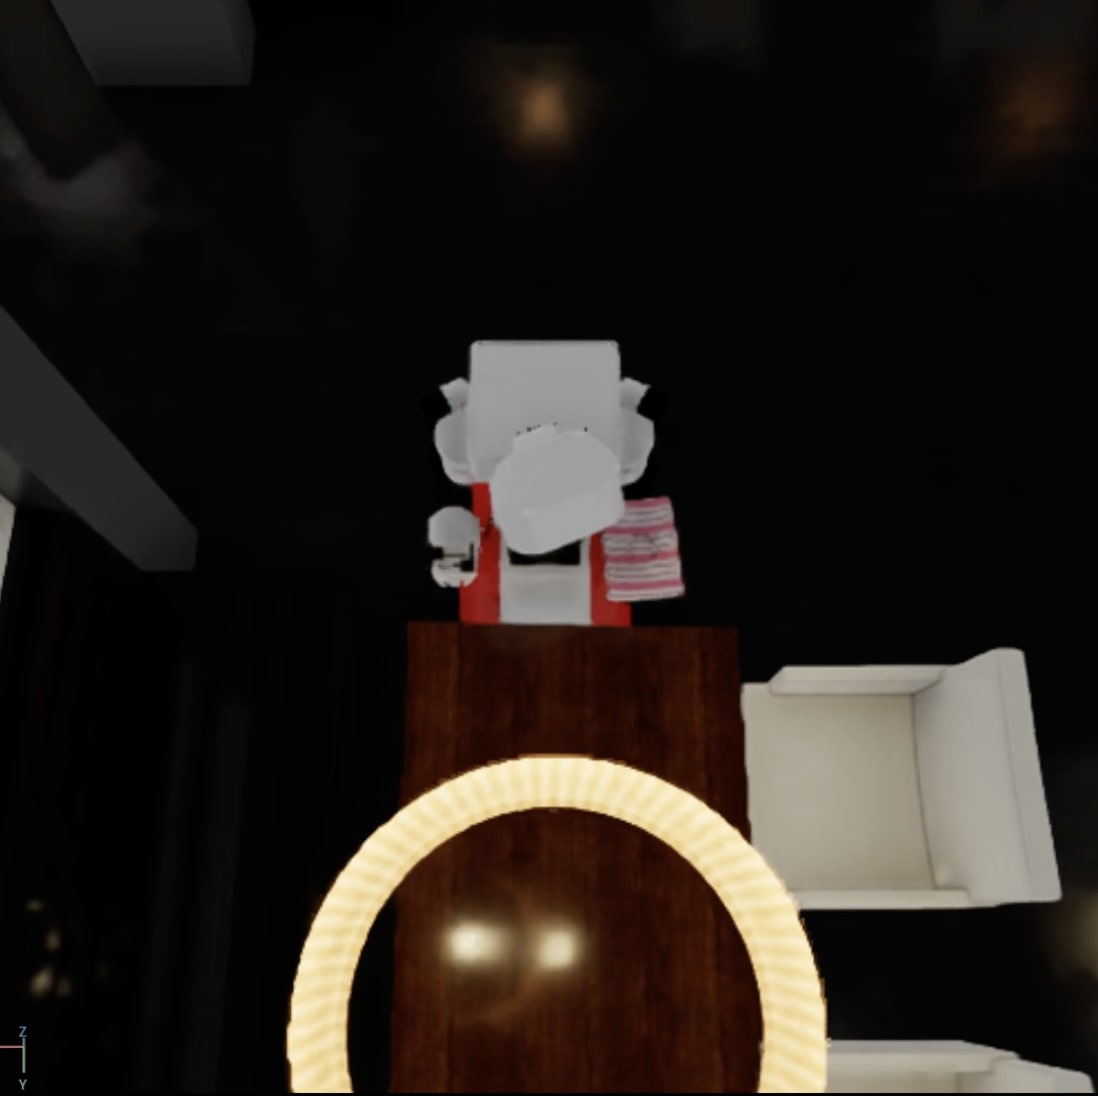
\includegraphics[width=0.3\linewidth]{figures/baseline_appendix/clean_table_1.png}&
%         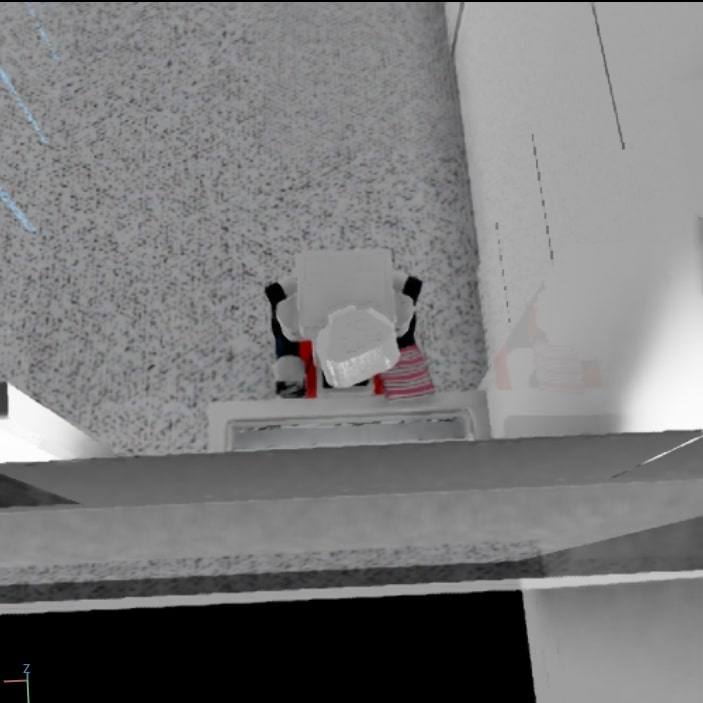
\includegraphics[width=0.3\linewidth]{figures/baseline_appendix/clean_table_2.png}&
%         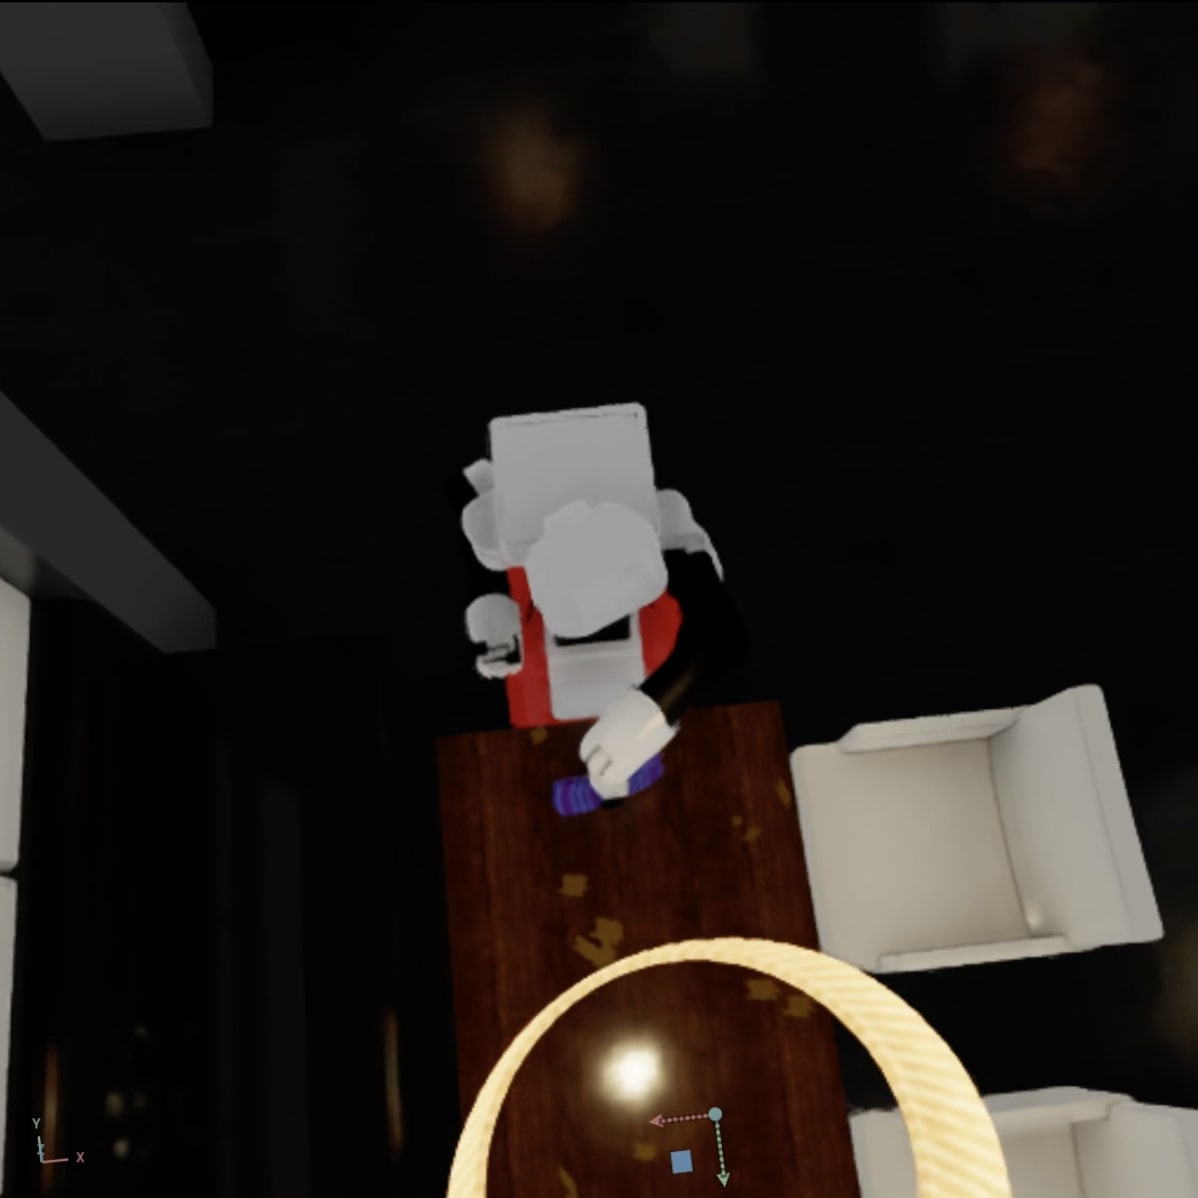
\includegraphics[width=0.3\linewidth]{figures/baseline_appendix/clean_table_3.png}\\
%         & c) Clean Table & \\
%     \end{tabular}
%     \caption{Overview of three tasks: \texttt{Store\_Decoration}, \texttt{Collect\_Trash}, and \texttt{Clean\_Table}.}
%     \label{fig:appendix_task}
% \end{minipage}
% \end{figure*}